\documentclass[12pt,a4paper]{report}

% Essential packages
\usepackage[utf8]{inputenc}
\usepackage[T1]{fontenc}
\usepackage{geometry}
\usepackage{setspace}
\usepackage{titlesec}
\usepackage{tocloft}
\usepackage{fancyhdr}
\usepackage{graphicx}
\usepackage{amsmath}
\usepackage{amsfonts}
\usepackage{newunicodechar}
\newunicodechar{⁻}{\textsuperscript{-}}
\usepackage{textcomp}
\usepackage{amssymb}
\usepackage{algorithm}
\usepackage{algorithmic}
\usepackage{listings}
\usepackage{xcolor}
\usepackage{booktabs}
\usepackage{array}
\usepackage{longtable}
\usepackage{multirow}
\usepackage{caption}
\usepackage{subcaption}
\usepackage{hyperref}
\usepackage{cleveref}
\usepackage{natbib}
\usepackage{url}
\usepackage{enumitem}

% Page geometry
\geometry{
    left=3cm,
    right=2.5cm,
    top=2.5cm,
    bottom=2.5cm
}

% Line spacing
\onehalfspacing

% Header and footer
\pagestyle{fancy}
\fancyhf{}
\fancyhead[R]{\thepage}
\fancyhead[L]{\leftmark}
\renewcommand{\headrulewidth}{0.4pt}

% Chapter and section formatting
\titleformat{\chapter}[display]
{\normalfont\Large\bfseries\centering}{\chaptertitlename\ \thechapter}{20pt}{\Large}
\titlespacing*{\chapter}{0pt}{0pt}{20pt}

% Hyperref settings
\hypersetup{
    colorlinks=true,
    linkcolor=black,
    filecolor=magenta,      
    urlcolor=blue,
    citecolor=black,
    pdftitle={Master's Synopsis},
    pdfauthor={Your Name},
}

% Custom commands
\newcommand{\university}{Indian Institute of Technology, Delhi}
\newcommand{\department}{Department of Applied Mechanics}
\newcommand{\degree}{Master of Science by Research}
\newcommand{\specialization}{Surrogate Modelling and Discrepancy Learning}
\newcommand{\thesistitle}{Multi-Fidelity Surrogate Modeling for Structural Response Prediction: Integrating 1D Zigzag Theory with Deep Learning for Enhanced Computational Efficiency}
\newcommand{\authorname}{Abhijit Roy Choudhury}
\newcommand{\rollnumber}{2023AMY7542}
\newcommand{\supervisor}{Dr. Rajdip Nayek}
\newcommand{\cosupervisor}{Dr. Souvik Chakroborty} 
\newcommand{\submissiondate}{Aug, 2025}

\begin{document}

\begin{titlepage}
\centering
\vspace*{-1.5cm}
% Top line
\rule{\textwidth}{0.6pt} \\[0.3cm]
% Title - Bigger and bold
{\LARGE \textbf{Multi-Fidelity Surrogate Modeling for Structural Response Prediction}}
{\LARGE \textbf{and Damage Parameterization:}}\\[0.25cm]
{\Large \textbf{Integrating 1D Zigzag Theory with Deep Learning for}}\\[0.08cm]
{\Large \textbf{Enhanced Computational Efficiency and Inverse Problem Solutions}} \\[0.3cm]
\rule{\textwidth}{0.6pt} \\[0.03cm]
% Report type
{\large \textsc{A SYNOPSIS REPORT}}\\[0.3cm]
{\normalsize Submitted in Partial Fulfillment of the Requirements\\
for the Degree of}\\[0.2cm]
{\large \textbf{Master of Science}}\\
{\large (by Research)}\\[0.08cm]
% Author details
\large by\\[0.2cm]
{\Large \textbf{Abhijit Roy Choudhury}}\\[0.08cm]
{\normalsize Roll No: \texttt{2023AMY7542}}\\
\texttt{amy237542@iitd.ac.in} \\[0.4cm]
% Supervisor details
{\normalsize Under the supervision of}\\[0.2cm]
{\large \textbf{Dr. Rajdip Nayek}}\\
{\large and}\\
{\large \textbf{Dr. Souvik Chakroborty}}\\[0.5cm]
% Institute Seal (logo placeholder)
\includegraphics[width=3.8cm]{iit.png} \\[0.5cm]
% Bottom info
{\large November 2025} \\[0.2cm]
{\large \textbf{Department of Applied Mechanics}}\\
{\large \textbf{Indian Institute of Technology Delhi}}
\end{titlepage}




% Abstract
\chapter*{Abstract}
\newpage
\addcontentsline{toc}{chapter}{Abstract}
% Add your abstract here - brief summary of the work, methodology, key findings

% Table of Contents
\tableofcontents
\newpage

% List of Figures
\listoffigures
\newpage

% List of Tables
\listoftables
\newpage

% List of Abbreviations (optional)
\chapter*{List of Abbreviations}
\addcontentsline{toc}{chapter}{List of Abbreviations}
\begin{tabular}{ll}
% AI & Artificial Intelligence \\
% ML & Machine Learning \\
% Add your abbreviations here
\end{tabular}
\newpage

% Main Content Begins
\pagenumbering{arabic}
\setcounter{page}{1}

% Chapter 1: Introduction
\chapter{Introduction}
\label{chap:introduction}

Structural response prediction constitutes a fundamental challenge in engineering analysis, where the persistent trade-off between computational accuracy and efficiency drives continuous methodological innovation. Modern engineering structures demand precise prediction of mechanical behavior under diverse loading and material conditions, yet traditional high-fidelity computational approaches often require prohibitive computational resources for real-time applications and design optimization scenarios. This computational burden has necessitated the development of multi-fidelity surrogate modeling techniques that can achieve both efficiency and accuracy through intelligent integration of machine learning methodologies.

One-dimensional zigzag theories, originally developed for composite laminated structures, have demonstrated exceptional accuracy in capturing complex deformation patterns while maintaining computational efficiency through reduced degrees of freedom. The Refined Zigzag Theory achieves near two-dimen
sional accuracy with one-dimensional computational cost through innovative displacement field representations that eliminate shear correction factors. The present research extends this theoretical framework to homogeneous aluminum beams with rectangular notches, treating geometric discontinuities as virtual interfaces through fictitious three-layer decomposition. This non-standard application offers two critical advantages: first, the virtual layer concept provides a natural and convenient framework for modeling rectangular notch geometries without requiring complex mesh adaptations or discontinuous elements; second, zigzag kinematics capture through-thickness displacement variations and local strain concentrations near notch regions while maintaining the computational efficiency characteristic of one-dimensional formulations.


Complementary two-dimensional plane strain finite element analysis establishes high-fidelity reference solutions through structured meshes employing biquadratic elements. The implementation utilizes intelligent matrix caching strategies, reusing assembled stiffness and mass matrices across parameter variations and applying localized modifications for notch representation through element property reduction. Explicit central difference time integration with GPU acceleration provides computational efficiency, while element removal techniques approximate void regions without requiring remeshing procedures while maintaining the required accuracy.

Contemporary advances in deep learning architectures have revolutionized surrogate modeling by enabling efficient capture of complex nonlinear relationships between input parameters and structural responses. Autoencoders, characterized by their encoder-decoder structure with latent space compression, prove exceptionally effective for dimensionality reduction of time-series structural responses. The integration of gradient boosting algorithms, particularly XGBoost, with autoencoder latent representations creates powerful surrogate models capable of rapid parameter-to-response mapping while addressing the curse of dimensionality inherent in direct regression approaches.

This research develops a comprehensive multi-fidelity surrogate modeling framework integrating one-dimensional zigzag theory with two-dimensional finite element analysis through transfer learning methodologies. The Low-Fidelity Surrogate Model employs non-conditional autoencoders trained on zigzag theory responses, learning compressed latent representations that capture essential response characteristics. XGBoost regression models subsequently map input parameters including notch geometry and material properties to these latent vectors, enabling direct parameter-to-response prediction through decoder reconstruction. The Multi-Fidelity Surrogate Model implements transfer learning by fine-tuning pre-trained low-fidelity components using limited high-fidelity data, preventing catastrophic forgetting while adapting latent space representations to capture systematic discrepancies between modeling approaches. For comparative validation, a High-Fidelity Surrogate Model trained exclusively on two-dimensional finite element data establishes baseline performance metrics, quantifying the advantages of transfer learning versus direct high-fidelity modeling.

The inverse problem formulation for structural health monitoring relies on estimating unknown notch parameters from measured dynamic responses. The multi-fidelity surrogate model serves as the computational backbone for this estimation, enabling efficient exploration of the parameter space through differential evolution optimization. By leveraging composite loss functions that balance reconstruction accuracy, correlation preservation, and frequency-domain matching, the surrogate model facilitates robust parameter recovery while accounting for model-reality mismatch Severity-based classification into damage categories establishes robust success criteria that account for model-reality mismatch, providing practical metrics for structural integrity assessment beyond precise parameter recovery.

The transfer learning approach represents a significant methodological advancement by leveraging learned representations from low-fidelity data before fine-tuning with limited high-fidelity examples. The methodology validates multi-fidelity advantages through systematic comparison against baseline approaches, demonstrating effective knowledge transfer that bridges the gap between computationally efficient one-dimensional models and accurate two-dimensional predictions. When applied to the inverse problem of parameter estimation, this framework enables efficient recovery of unknown structural characteristics from measured responses without prohibitive computational costs. The research establishes foundations for real-time structural health monitoring, where rapid damage assessment through reduced-order surrogate models enables autonomous inspection and predictive maintenance capabilities previously constrained by computational limitations.



\section{Motivation}
\label{sec:motivation}
Surrogate models have emerged as a critical approach to address the computational limitations of high-fidelity simulations in structural dynamics applications. Surrogate models provide computationally cheaper approximations that enable efficient exploration of complex parameter spaces in finite element model updating, where the high computational costs of fine-mesh numerical models would otherwise prohibit large-scale inverse analysis \href{https://doi.org/10.1155/2019/8086024}{[1]}. Multi-fidelity surrogate modeling approaches leverage both low-fidelity and high-fidelity model data within hierarchical frameworks, improving both computational efficiency and predictive accuracy by combining the computational economy of reduced-order models with the accuracy constraints of detailed simulations \href{https://doi.org/10.1002/eqe.3839}{[2]}\href{https://doi.org/10.1002/2475-8876.70002}{[3]}
 Physics-informed neural networks have emerged as a powerful tool for solving partial differential
  equations in engineering mechanics, demonstrating the ability to incorporate physical laws directly into the
  learning process\href{https://www.sciencedirect.com/science/article/pii/S0021999118307125}{[4]}. Recent applications in solid mechanics have shown promising results, though specific error
   rates vary depending on problem complexity and network architecture \href{https://epubs.siam.org/doi/10.1137/19M1274067}{[5]}. However, critical research gaps persist in applying these methods to homogeneous structures with geometric discontinuities. Conventional surrogate models demonstrate substantially degraded performance when problem dimensionality exceeds 20 parameters, requiring exponentially more training samples to maintain accuracy \href{https://onlinelibrary.wiley.com/doi/10.1002/cnm.2985}{[7]}.  The engineering significance extends far beyond computational gains, as these multi-fidelity approaches enable real-time structural health monitoring for critical infrastructure, autonomous damage detection systems, and predictive maintenance frameworks that were previously computationally intractable.\href{https://www.sciencedirect.com/science/article/pii/S0888327023002832}{[8]}
 Research from 2020-2025 demonstrates exponential growth in applications, with marine and aerospace sectors leading adoption due to the critical need for continuous structural monitoring in harsh environments.\href{https://doi.org/10.3390/s20102778}{[9]}
 The mathematical foundation built on established theories like the Kapuria-Hagedorn framework and Refined Zigzag Theory provides the necessary theoretical rigor\href{http://dx.doi.org/10.2140/jomms.2007.2.1267}{[10]},while emerging machine learning integration strategies offer unprecedented opportunities for bridging classical structural mechanics with modern computational approaches.

The mathematical foundation for multi-fidelity structural analysis rests on well-established theories that have demonstrated exceptional accuracy and efficiency across diverse applications. Refined Zigzag Theory (RZT) maintains constant degrees of freedom regardless of layer count while eliminating the need for transverse-shear correction factors, making it ideally suited as a low-fidelity model in multi-fidelity frameworks.\href{https://www.sciencedirect.com/science/article/pii/S0263822315006819}{[11]} The theory's multi-scale approach expresses in-plane displacement fields as superpositions of coarse and fine contributions\href{https://www.sciencedirect.com/science/article/pii/S0263822315006819}{[11]}\href{https://link.springer.com/article/10.1007/s11012-015-0222-0}{[12]}, enabling efficient capture of layerwise effects without computational penalties. The Kapuria-Hagedorn framework offers a unified, efficient formulation for layerwise theories, capturing both extension and shear effects using third-order zigzag axial displacement with only three primary variables.\href{http://dx.doi.org/10.2140/jomms.2007.2.1267}{[10]} This significantly reduces computational complexity while preserving physical accuracy, making it well-suited for integration with machine learning models that benefit from low-dimensional parametric representations\href{https://www.sciencedirect.com/science/article/pii/S0045793018304250}{[13]}.
Recent extensions of the Refined Zigzag Theory (RZT) to homogeneous materials with geometric discontinuities—such as aluminum plates with rectangular notches—treat these discontinuities as virtual interfaces via infinitesimal perturbations in the transverse shear stiffness of the medium [\href{https://link.springer.com/article/10.1007/s11012-015-0222-0}{[12]}, . This approach, developed to circumvent the need for shear correction factors, enables the use of zigzag kinematics in otherwise homogeneous media, though its application to complex geometric discontinuities remains an active area of research.
Advances in mixed-dimensional coupling between 1D beam theories and 2D finite elements have shown strong potential, offering accuracy and computational efficiency without introducing spurious stresses at transition \href{https://publications.rwth-aachen.de/record/854218/files/854218.pdf?}{[14]}. However, standardization and commercial integration of these methods remain limited\href{https://doi.org/10.1115/1.1557614}{[15]}.
Modeling notches as virtual layer discontinuities is particularly promising, allowing for slope discontinuities while maintaining displacement continuity. Though validated for end-notched and V-notched beams, its application to rectangular notches in homogeneous aluminum beams remains an open area for further assessment \href{https://www.sciencedirect.com/science/article/pii/S0022460X24000774}{[16]}\href{https://research.sabanciuniv.edu/id/eprint/41426/1/10222508_Tabrizi_Isa_Emami.pdf}{[17]}.

The period 2020-2025 has witnessed paradigmatic shifts in finite element methodology, with FEM-enhanced neural networks (FEM-NN) emerging as the most significant breakthrough\href{https://www.sciencedirect.com/science/article/pii/S2352012422000947}{[18]}. These physics-conforming surrogate models eliminate expensive pre-calculated simulation datasets by incorporating discretized PDE forms directly into loss functions\href{https://amses-journal.springeropen.com/articles/10.1186/s40323-023-00243-1}{[19]}. Computational efficiency gains have been substantial across multiple fronts. Modern GPU acceleration implementations achieve sub-second matrix assembly for 3-million degree-of-freedom systems, while commercial solutions like Ansys Mechanical 2025 R2 demonstrate up to 13× speedup on large transient models through mixed solver approaches\href{https://onlinelibrary.wiley.com/doi/pdf/10.1002/nme.6383}{[20]}\href{https://metavo.metacentrum.cz/export/sites/meta/cs/seminars/seminar5/Ansys-SVSFEM.pdf}{[21]}. The emergence of AI-integrated workflows, including Ansys Copilot for in-context engineering support, signals the democratization of advanced simulation capabilities. 

For structures with notches and discontinuities, geometrically exact beam theory with embedded strong discontinuities (Tojaga et al., 2023) provides breakthrough capabilities for failure modeling with large deformations\href{https://www.sciencedirect.com/science/article/pii/S0045782523001378}{[22]}. Steel fiber reinforced concrete beam-column joints analyzed through advanced FEM show less than 5\% average error under cyclic loading, with optimal 2\% steel fiber volume fractions delivering 15\% increased load capacity and 25\% delayed crack formation\href{https://www.nature.com/articles/s41598-024-69270-1}{[23]}. Comparative studies between 1D and 2D approaches reveal nuanced trade-offs. Higher-order beam theories maintain computational efficiency while addressing limitations of classical Euler-Bernoulli and Timoshenko approaches for thin-walled structures\href{https://www.sciencedirect.com/science/article/pii/S2352012420303854}{[24]}\href{https://www.sciencedirect.com/science/article/pii/S0020740322000649#sec0015}{[25]}. Beam element models excel for slender structures and global response analysis, while 2D/3D elements become essential for local stress concentrations and complex geometries, with hybrid approaches emerging as optimal strategies for balancing accuracy and computational cost\href{Cook, R. D., Malkus, D. S., Plesha, M. E., & Witt, R. J. (2001). Concepts and Applications of Finite Element Analysis (4th ed.). John Wiley & Sons.}{[26]}.

The integration of deep learning architectures with structural engineering has produced transformative advances across multiple fronts\href{https://doi.org/10.3390/s20102778}{[27]}, with conditional autoencoders achieving 35\% improvement in minor damage detection accuracy through mechanics-informed approaches\href{https://arxiv.org/html/2402.15492v1}{[28]}.The breakthrough MIDAS (Mechanics-Informed Damage Assessment of Structures) framework introduced by Li et al. in 2024 integrates mechanical characteristics directly into neural network architectures through pairwise mechanical loss terms, enabling real-time adaptation with only three hours of training data. \href{https://doi.org/10.1038/s41467-024-52501-4}{[29]} This represents a fundamental shift from traditional data-driven approaches toward physics-aware machine learning systems that respect underlying structural mechanics principles. 
U-Net architectures have demonstrated exceptional performance in structural field prediction and discrepancy learning applications, particularly when enhanced with attention mechanisms and skip connections\href{https://www.sciencedirect.com/science/article/pii/S0955598622001753}{[30]}. Recent research shows these architectures excel at multi-scale feature extraction through encoder-decoder frameworks while preserving spatial information crucial for structural applications. Microstructure-embedded autoencoder approaches using U-Net-like architectures achieve superior performance over standard methods by reconstructing high-resolution solution fields from reduced parametric spaces\href{https://doi.org/10.1007/s00466-024-02568-z}{[31]}, directly addressing the multi-fidelity integration challenge central to this research domain. 
XGBoost integration in surrogate modeling has proven particularly effective for structural parameter mapping, with Bayesian-optimized XGBoost models achieving 8x faster hyperparameter optimization compared to traditional methods while maintaining superior performance.\href{https://doi.org/10.1016/j.engstruct.2023.117307}{[32]} The algorithm's ability to handle feature interactions and collinearity makes it especially suitable for the parameter mapping stage in multi-fidelity frameworks, where complex relationships between low-fidelity model parameters and high-fidelity discrepancies must be captured efficiently.\href{https://www.researchgate.net/figure/The-performance-of-XGBoost-surrogate-models-in-the-training-and-testing-for-predicting_fig5_372412960}{[33]}

Multi-fidelity modeling has matured from theoretical concept to practical engineering tool, with documented applications showing orders of magnitude improvements in computational efficiency while maintaining engineering accuracy requirements \href{https://doi.org/10.3934/acse.2023015}{[34]}  These achievements stem from sophisticated integration strategies that combine additive and multiplicative correction methods, hierarchical modeling approaches, and advanced discrepancy learning techniques.
 This dramatic improvement results from sophisticated discrepancy learning methodologies that capture complex mappings between fidelity levels through ensemble-based approaches using multiple deep neural networks with Bayesian optimization. The integration of online transfer learning methods enables real-time model updates, addressing the critical need for adaptive systems in operational environments.\href{https://doi.org/10.1016/j.aei.2022.101689}{[35]}\href{http://dx.doi.org/10.3390/ecsa-9-13344}{[36]}


Wave-based structural health monitoring (SHM) has matured significantly, leveraging guided waves in the 20 kHz–1 MHz range, with optimal performance typically between 10s and 100s kHz\href{https://royalsocietypublishing.org/doi/abs/10.1098/rspa.2007.0048}{[37]}. Hanning-windowed 5-cycle sine bursts at 100 kHz are widely used for efficient large-area monitoring\href{https://www.sciencedirect.com/science/article/pii/S0020740322004921}{[38]}.
Advances such as physics-guided neural networks and optimized baseline selection have improved signal processing, but environmental effects like temperature variation still complicate damage detection and increase computational demands. Long-term monitoring also generates massive datasets—up to 9 TB over 4.5 years—posing challenges for storage and wireless data transmission\href{https://pmc.ncbi.nlm.nih.gov/articles/PMC12162875/}{[39]}\href{https://www.researchgate.net/publication/359193759_Temperature_variation_compensated_damage_classification_and_localisation_in_ultrasonic_guided_wave_SHM_using_self-learnt_features_and_Gaussian_mixture_models}{[40]}.
Recent research demonstrates that transfer learning substantially improves the feasibility of real-time damage assessment across multiple applications. Transfer learning can reduce training data requirements by at least 25\% when applied to new scenarios, while simultaneously improving model accuracy by over 26\%\href{https://onlinelibrary.wiley.com/doi/10.1111/mice.12674}{[41]}. For probabilistic damage prediction in composites, machine learning models achieved speedups exceeding 11 times over competing algorithms while maintaining over 99\% accuracy in failure envelope predictions\href{https://4spepublications.onlinelibrary.wiley.com/doi/10.1002/pc.27144}{[42]}. More significantly, energy-based deep learning frameworks with transfer learning achieve a tenfold reduction in response data requirements and enhance training efficiency by 7.4 times, making rapid probabilistic assessment feasible at regional scales\href{https://onlinelibrary.wiley.com/doi/10.1002/eqe.4331}{[43]}. Regional seismic damage assessment using LSTM models operates in 0.52 seconds on average, compared to over 1,500 times greater computational resources required by traditional nonlinear time-history analysis methods, demonstrating that transfer learning-based approaches now enable real-time probabilistic damage assessment\href{https://onlinelibrary.wiley.com/doi/10.1111/mice.12628}{[44]}.  

Inverse problems in structural engineering involve determining unknown system parameters such as damage locations, crack depths, or dynamic loads from measured structural responses, fundamentally differing from forward problems where structural behavior is predicted from known parameters \href{https://www.tandfonline.com/doi/full/10.1080/17415970500272908}{[45]}. The crack detection inverse problem can be formulated by providing geometry, material properties, boundary conditions, and measured system responses with inherent noise to identify crack locations and depths \href{https://www.researchgate.net/publication/239403302_Inverse_and_Crack_Identification_Problems_in_Engineering_Mechanics}{[46]}. These problems are inherently ill-posed due to multimodality, high-dimensional variables, and sensitivity to measurement errors, necessitating regularization methods that incorporate constraining factors to stabilize solutions. Tikhonov regularization has emerged as a classical approach for addressing ill-conditioned inverse problems by adding penalty terms to stabilize matrix inversions, with modifications including adaptive regularization schemes that discriminate between damaged and undamaged elements through iterative side conditions \href{https://www.sciencedirect.com/science/article/pii/S088832701000052X}{[47]}\href{https://onlinelibrary.wiley.com/doi/10.1002/cnm.541}{[48]}. Optimization algorithms have become indispensable for solving these inverse problems, with Genetic Algorithms providing robust global search capabilities for crack parameter identification despite computational expense \href{https://www.sciencedirect.com/science/article/pii/S1568494607001020}{[48]}, while Particle Swarm Optimization offers faster convergence through collaborative swarm intelligence mechanisms, particularly effective when hybridized with simplex methods for damage detection in beam and truss structures \href{https://www.sciencedirect.com/science/article/pii/S0965997809000040}{[49]}. More recent developments have integrated deep learning approaches, where Convolutional Neural Networks automatically learn crack-related features from raw sensor data without manual feature extraction, achieving detection accuracies exceeding 98\% for concrete crack identification, and encoder-decoder architectures such as U-Net enable pixel-level crack segmentation from wavefield measurements in plate structures. These machine learning methods address computational limitations of traditional optimization by creating surrogate models that rapidly predict structural responses, though they require extensive training datasets and may struggle with generalization to unseen damage patterns \href{https://www.nature.com/articles/s41467-024-52501-4}{[50]}. The integration of physics-informed constraints with data-driven approaches represents an emerging paradigm that balances computational efficiency with physical interpretability for structural health monitoring applications.

\section{Research Objectives}

The primary objectives of this research address the development and validation of a multi-fidelity surrogate modeling framework for structural response prediction in notched beam configurations, systematically integrating one-dimensional zigzag theory with two-dimensional finite element analysis through machine learning architectures. The secondary objective encompasses the application of this multi-fidelity surrogate modeling framework to solve the inverse problem of notch parameters identification in the beam structures using differential evolution algorithms, enabling efficient and accurate estimation of unknown notch properties from 2D beam response data without the computational burden of repeated high-fidelity finite element analyses.

\bigskip

\noindent\textbf{Objective 1: Dual-Fidelity Computational Framework Development}

\medskip

\textbf{1a. One-Dimensional Zigzag Beam Model for Notched Homogeneous Beams:} Extend Refined Zigzag Theory to homogeneous aluminum beams with rectangular notches through fictitious three-layer decomposition, implementing finite element discretization with adaptive meshing near notch boundaries. Develop ultrasonic wave propagation simulation capabilities at specified excitation frequency with sensor variation response capture, generating extensive parametric datasets spanning notch geometric variations and material property ranges for surrogate model training.

\medskip

\textbf{1b. Two-Dimensional Plane Strain Finite Element Reference Model:} Establish high-fidelity reference solutions through structured biquadratic element meshes with intelligent matrix caching strategies for computational efficiency. Implement element removal techniques for notch representation without remeshing, utilizing GPU-accelerated explicit time integration to generate limited high-fidelity datasets with sensor configurations matched to low-fidelity implementations for direct comparison and training. .

\bigskip

\textbf{Objective 2: Machine Learning Surrogate Architecture Development}

\medskip

\textbf{2a: Low-Fidelity Surrogate Model (LFSM):} Develop autoencoder-based dimensionality reduction architecture to compress high-dimensional time-series responses into compact latent representations, training exclusively on one-dimensional zigzag theory data. Implement XGBoost regression for parameter-to-latent mapping from notch related parameters, material and response point inputs, enabling rapid structural response prediction through decoder reconstruction without executing numerical simulations.

\medskip

\textbf{2b: Multi-Fidelity Surrogate Model (MFSM) through Transfer Learning:} Implement transfer learning methodology by fine-tuning pre-trained LFSM autoencoder components using limited two-dimensional finite element data exclusively, employing conservative learning rates and elevated loss weighting to prevent catastrophic forgetting. Retrain XGBoost models exclusively on latent representations extracted from high-fidelity two-dimensional responses, creating surrogate models that leverage knowledge transferred from extensive low-fidelity pre-training while adapting to capture the systematic discrepancies between modeling fidelities through limited high-fidelity data.


\bigskip

\textbf{Objective 3: Inverse Problem Formulation for Structural Health Monitoring}

\medskip

Develop an inverse solver to estimate notch parameters (location, depth, width) from measured ultrasonic wave responses using the trained MFSM as the forward model. The inverse problem treats high-fidelity two-dimensional finite element responses as ground truth measurements, with differential evolution optimization iteratively proposing parameter candidates, executing the MFSM forward model to generate predicted responses, and computing composite loss functions. The optimization continues iteratively until parameter predictions converge, minimizing discrepancies between MFSM-predicted responses and two-dimensional ground truth measurements. Establish a severity-based damage classification framework (mild, moderate, severe) prioritizing correct severity identification over exact geometric parameter recovery to account for model-reality mismatch. Validate inverse problem performance through systematic testing on high-fidelity two-dimensional response data, reporting parameter estimation accuracy and severity classification success rates to demonstrate feasibility for real-time structural health monitoring applications.





% Chapter 2: Theoretical Foundation
\chapter{Theoretical Foundation and Concepts}
\label{chap:foundation}

\section{1D Beam Zigzag Theory}
\label{sec:zigzag_theory}
The zigzag theory for laminated composite beams represents a sophisticated refinement of classical beam theories that addresses the inherent limitations of traditional approaches when dealing with layered structures. Unlike classical theories that assume linear displacement variation through the beam thickness, zigzag theory incorporates the material discontinuities between layers by allowing piecewise-linear displacement patterns that capture the sudden changes in material properties at layer interfaces.

Consider a laminated composite beam of total height $h$ consisting of $N$ perfectly bonded layers, where each layer $k$ extends from coordinate $z_{k-1}$ to $z_k$ measured from a reference plane. The beam extends along the longitudinal $x$-direction with length $L$, while the $z$-direction represents the through-thickness coordinate. The fundamental assumption underlying zigzag theory is that the axial displacement exhibits a layerwise linear variation that accounts for the transverse shear deformation effects neglected in classical beam theories.

The theory assumes that each layer behaves as a linear elastic material with distinct material properties, creating interfaces where material properties change discontinuously. These material discontinuities generate interlaminar shear stress concentrations that classical theories cannot accurately predict. The zigzag approach addresses this limitation by introducing a zigzag function that captures the layer-dependent linear variation of axial displacement while maintaining displacement continuity across layer interfaces.

For the specific case of three-layer composite beams under consideration, the layers are designated as bottom ($k=1$), middle ($k=2$), and top ($k=3$), with interfaces located at $z_1$ and $z_2$. Each layer possesses distinct elastic moduli $E^{(k)}$, shear moduli $G^{(k)}$, and densities $\rho^{(k)}$, while maintaining perfect bonding at all interfaces.

The displacement field in zigzag theory is expressed through three primary kinematic variables that represent the global beam behavior, enhanced by a zigzag function that captures local layer effects. The axial displacement $u(x,z,t)$ is formulated as:

\begin{equation}
    u(x,z,t) = u_0(x,t) - z \frac{\partial w_0}{\partial x}(x,t) + R^{(k)}(z) \, \psi_0(x,t)
\end{equation}


where \(u_0(x,t)\) represents the axial displacement of the reference plane located at \(z = 0\), \(w_0(x,t)\) denotes the transverse displacement, and \(\psi_0(x,t)\) is the shear deformation parameter related to the average shear strain of the reference plane. The term \(- z \frac{\partial w_0}{\partial x}\)

represents the classical Euler--Bernoulli contribution, while $R^{(k)}(z)$ is the layer-dependent zigzag function.

The transverse displacement is assumed to remain constant across the beam thickness, consistent with the assumption of inextensible normals:
\begin{equation}
   w(x,z,t) = w_0(x,t) 
\end{equation}


This assumption is valid for slender beams where the length-to-thickness ratio is sufficiently large, typically greater than $10$. For the analysis of ultrasonic wave propagation in composite beams, this assumption remains appropriate given the high frequency content and the associated short wavelengths relative to beam thickness.

The displacement field can be expressed in compact matrix form as:

\begin{equation}
\mathbf{u}(x,z,t) = 
\begin{Bmatrix}
u(x,z,t) \\
w(x,z,t)
\end{Bmatrix}
=
\begin{bmatrix}
1 & -z\frac{\partial }{\partial x} & R^{(k)}(z) \\
0 & 1 & 0
\end{bmatrix}
\begin{Bmatrix}
u_0(x,t) \\
w_0(x,t) \\
\psi_0(x,t)
\end{Bmatrix}
\end{equation}


This formulation reduces the infinite degrees of freedom associated with the continuum displacement field to three generalized displacement variables, enabling efficient computational implementation while maintaining the essential physics of layered beam behavior.

\begin{figure}[htbp]
\centering
\includegraphics[width=\textwidth]{zigzaglayer.png}
\caption{Schematic Representation of an
N-Layer Laminated Composite Beam}
\label{fig:zigzag_layer}
\end{figure}

The strain components relevant to beam theory are the axial strain $\varepsilon_x$ and the transverse shear strain $\gamma_{xz}$. These strains are derived from the displacement field through standard kinematic relations.

The axial strain is obtained as:
\begin{equation}
\varepsilon_x = \frac{\partial u}{\partial x} 
= \frac{\partial u_0}{\partial x} 
- z \frac{\partial^2 w_0}{\partial x^2} 
+ R^{(k)}(z) \frac{\partial \psi_0}{\partial x}
\end{equation}

This expression reveals the three distinct contributions to axial strain: the membrane strain 
$\frac{\partial u_0}{\partial x}$, the bending strain 
$- z \frac{\partial^2 w_0}{\partial x^2}$, and the zigzag contribution 
$R^{(k)}(z) \frac{\partial \psi_0}{\partial x}$ that captures the layer-wise linear variation.

The transverse shear strain is formulated as:
\begin{equation}
\gamma_{xz} = \frac{\partial u}{\partial z} + \frac{\partial w}{\partial x} 
= \frac{\partial R^{(k)}}{\partial z} \, \psi_0 
\end{equation}

Since the transverse displacement is independent of $z$, the shear strain depends only on the derivative of the zigzag function. The term 
$\frac{\partial R^{(k)}}{\partial z}$ represents the layer-wise constant shear strain within each layer, while maintaining the necessary discontinuities at layer interfaces to accommodate different material properties.

The strain field can be expressed in matrix notation as:
\begin{equation}
\begin{Bmatrix} \varepsilon_x \\ \gamma_{xz} \end{Bmatrix} =
\begin{bmatrix} 
\frac{\partial}{\partial x} & -z \frac{\partial^2}{\partial x^2} & R^{(k)}(z) \frac{\partial}{\partial x} \\
0 & 0 & \frac{\partial R^{(k)}}{\partial z} 
\end{bmatrix}
\begin{Bmatrix} u_0 \\ w_0 \\ \psi_0 \end{Bmatrix}
\end{equation}


The zigzag function $R^{(k)}(z)$ must satisfy several critical conditions to ensure physical consistency and mathematical well-posedness. These conditions include displacement continuity at layer interfaces, stress continuity requirements, and appropriate boundary conditions at the beam's top and bottom surfaces.

For a three-layer beam, the zigzag function is constructed as a piecewise cubic polynomial within each layer:
\begin{equation}
R^{(k)}(z) = a_0^{(k)} + a_1^{(k)} z + a_2^{(k)} z^2 + a_3^{(k)} z^3
\end{equation}

where the coefficients $a_0^{(k)}$, $a_1^{(k)}$, $a_2^{(k)}$, and $a_3^{(k)}$ are determined through the enforcement of continuity and boundary conditions.

The fundamental continuity conditions require that the axial displacement remains continuous across layer interfaces. At the interface between layers $k$ and $k+1$ located at $z = z_k$, this condition yields:
\begin{equation}
R^{(k)}(z_k) = R^{(k+1)}(z_k)
\end{equation}

Additionally, the transverse shear stress must remain continuous across interfaces to maintain equilibrium. This condition is expressed as:
\begin{equation}
G^{(k)} \gamma_{xz}^{(k)} = G^{(k+1)} \gamma_{xz}^{(k+1)} \quad \text{at} \quad z = z_k
\end{equation}

Substituting the shear strain expression, this becomes:
\begin{equation}
G^{(k)} \frac{\partial R^{(k)}}{\partial z}\bigg|_{z=z_k} = 
G^{(k+1)} \frac{\partial R^{(k+1)}}{\partial z}\bigg|_{z=z_k}
\end{equation}

The boundary conditions at the top and bottom surfaces require that the transverse shear stress vanishes for a free surface:
\begin{equation}
\gamma_{xz}^{(1)}\bigg|_{z=z_0} = \frac{\partial R^{(1)}}{\partial z}\bigg|_{z=z_0} \, \psi_0 = 0
\end{equation}

\begin{equation}
\gamma_{xz}^{(N)}\bigg|_{z=z_N} = \frac{\partial R^{(N)}}{\partial z}\bigg|_{z=z_N} \, \psi_0 = 0
\end{equation}

The determination of the zigzag function coefficients requires establishing a system of twelve equations to uniquely define the twelve unknown coefficients. This system incorporates displacement continuity conditions at layer interfaces, shear stress continuity requirements, boundary conditions at free surfaces, and appropriate normalization constraints.
The systematic solution of this constraint system yields the explicit expressions for the zigzag function coefficients in each layer. These coefficients define the piecewise cubic polynomials that capture the layer-wise linear variation of axial displacement while maintaining all necessary continuity and equilibrium requirements. The resulting zigzag functions completely characterize the enhanced displacement field and enable accurate representation of the through-thickness shear deformation behavior in laminated composite beams.



\subsection{Constitutive Relations for Composite Layers}

The constitutive relations for each layer relate the stress components to the strain components through the material properties. For each layer $k$, assuming isotropic material behavior within the layer, the stress-strain relations are:

\begin{align}
\sigma_x^{(k)} &= E^{(k)} \, \varepsilon_x^{(k)} \\
\tau_{xz}^{(k)} &= G^{(k)} \, \gamma_{xz}^{(k)}
\end{align}



where $E^{(k)}$ and $G^{(k)}$ are the elastic and shear moduli of layer $k$, respectively. For isotropic materials, the shear modulus is related to the elastic modulus through:

\begin{equation}
G^{(k)} = \frac{E^{(k)}}{2 \left( 1 + \nu^{(k)} \right)}
\end{equation}


where $\nu^{(k)}$ is Poisson's ratio for layer $k$.

Substituting the strain expressions into the constitutive relations yields:

\begin{equation}
\sigma_x^{(k)} = E^{(k)} \left[ 
\frac{\partial u_0}{\partial x} 
- z \frac{\partial^2 w_0}{\partial x^2} 
+ R^{(k)}(z) \frac{\partial \psi_0}{\partial x} 
\right]
\end{equation}


\begin{equation}
\tau_{xz}^{(k)} = G^{(k)} \left[ 
\frac{\partial R^{(k)}}{\partial z} \, \psi_0 
\right]
\end{equation}


These expressions reveal how the zigzag theory naturally captures the layer-wise variation of stresses while maintaining the necessary continuity conditions at interfaces.

\subsection{Variational formulation and governing equations}
\label{sec:variational}


The governing equations for the zigzag beam theory are derived using Hamilton's principle, which states that the motion of a dynamic system between two specified times makes the action integral stationary. For conservative systems, Hamilton's principle is formulated as:

\begin{equation}
\delta \int_{t_1}^{t_2} L \, dt = 0
\end{equation}

where the Lagrangian is given by
\begin{equation}
L = T - U
\end{equation}
representing the difference between the kinetic energy $T$ and the strain energy $U$. The variational operator $\delta$ denotes the first variation of the action integral with respect to the generalized coordinates.

\subsection*{Kinetic Energy Formulation}

The kinetic energy for a three-layer zigzag beam of length $L$ and width $b$ is expressed as:

\begin{equation}
T = \frac{1}{2} \int_0^L \int_{z_0}^{z_3} \rho^{(k)} 
\left[ \left(\frac{\partial u}{\partial t}\right)^2 
     + \left(\frac{\partial w}{\partial t}\right)^2 \right] 
\, b \, dz \, dx
\end{equation}

where $\rho^{(k)}$ denotes the density of layer $k$.  
Substituting the zigzag displacement field expressions:

\begin{align}
u(x,z,t) &= u_0(x,t) - z \frac{\partial w_0}{\partial x}(x,t) 
           + R^{(k)}(z) \, \psi_0(x,t) \\[6pt]
w(x,z,t) &= w_0(x,t)
\end{align}

and performing the through-thickness integration yields:

\begin{align}
T = \frac{1}{2} \int_0^L \Big[ & I_{00}\dot{u}_0^2 + I_{00}\dot{w}_0^2 
+ I_{11}\left(\frac{\partial \dot{w}_0}{\partial x}\right)^2 + I_{22}\dot{\psi}_0^2 \nonumber \\
& - 2I_{01}\dot{u}_0\frac{\partial \dot{w}_0}{\partial x} 
+ 2I_{02}\dot{u}_0\dot{\psi}_0 
- 2I_{12}\frac{\partial \dot{w}_0}{\partial x}\dot{\psi}_0 \Big] dx
\end{align}


The inertia coefficients are defined through layerwise integration:

\begin{align}
I_{00} &= \sum_{k=1}^{3} \rho^{(k)} b \int_{z_{k-1}}^{z_k} dz 
       = \sum_{k=1}^{3} \rho^{(k)} b \, h^{(k)} \\[6pt]
I_{01} &= \sum_{k=1}^{3} \rho^{(k)} b \int_{z_{k-1}}^{z_k} z \, dz \\[6pt]
I_{02} &= \sum_{k=1}^{3} \rho^{(k)} b \int_{z_{k-1}}^{z_k} R^{(k)}(z) \, dz \\[6pt]
I_{11} &= \sum_{k=1}^{3} \rho^{(k)} b \int_{z_{k-1}}^{z_k} z^2 \, dz \\[6pt]
I_{12} &= \sum_{k=1}^{3} \rho^{(k)} b \int_{z_{k-1}}^{z_k} z \, R^{(k)}(z) \, dz \\[6pt]
I_{22} &= \sum_{k=1}^{3} \rho^{(k)} b \int_{z_{k-1}}^{z_k} \left[ R^{(k)}(z) \right]^2 dz
\end{align}
where 
\begin{equation}
h^{(k)} = z_k - z_{k-1}
\end{equation}
represents the thickness of layer $k$.

\subsection*{Strain Energy Formulation}

The strain energy is expressed in terms of the stress and strain components:

\begin{equation}
U = \frac{1}{2} \int_0^L \int_{z_0}^{z_3} 
\left( \sigma_x^{(k)} \, \varepsilon_x^{(k)} 
     + \tau_{xz}^{(k)} \, \gamma_{xz}^{(k)} \right) 
b \, dz \, dx
\end{equation}

Substituting the constitutive relations and strain expressions, and performing the through-thickness integration yields:

\begin{align}
U = \frac{1}{2} \int_0^L &\Bigg[ 
A_{11} \left(\frac{\partial u_0}{\partial x}\right)^2 
+ A_{22} \left(\frac{\partial^2 w_0}{\partial x^2}\right)^2 
+ A_{33} \left(\frac{\partial \psi_0}{\partial x}\right)^2 
+ A_{44} \, \psi_0^2 \nonumber \\[6pt]
&- 2A_{12} \frac{\partial u_0}{\partial x} \frac{\partial^2 w_0}{\partial x^2} 
+ 2A_{13} \frac{\partial u_0}{\partial x} \frac{\partial \psi_0}{\partial x} 
- 2A_{23} \frac{\partial^2 w_0}{\partial x^2} \frac{\partial \psi_0}{\partial x}
\Bigg] dx
\end{align}

The stiffness coefficients are defined as:

\begin{align}
A_{11} &= \sum_{k=1}^{3} E^{(k)} b \int_{z_{k-1}}^{z_k} dz \\[6pt]
A_{12} &= \sum_{k=1}^{3} E^{(k)} b \int_{z_{k-1}}^{z_k} z \, dz \\[6pt]
A_{13} &= \sum_{k=1}^{3} E^{(k)} b \int_{z_{k-1}}^{z_k} R^{(k)}(z) \, dz \\[6pt]
A_{22} &= \sum_{k=1}^{3} E^{(k)} b \int_{z_{k-1}}^{z_k} z^2 \, dz \\[6pt]
A_{23} &= \sum_{k=1}^{3} E^{(k)} b \int_{z_{k-1}}^{z_k} z \, R^{(k)}(z) \, dz \\[6pt]
A_{33} &= \sum_{k=1}^{3} E^{(k)} b \int_{z_{k-1}}^{z_k} \left[R^{(k)}(z)\right]^2 dz \\[6pt]
A_{44} &= \sum_{k=1}^{3} G^{(k)} b \int_{z_{k-1}}^{z_k} \left[ \frac{\partial R^{(k)}}{\partial z} \right]^2 dz
\end{align}


\subsection*{Derivation of Governing Equations}

Application of Hamilton's principle to the Lagrangian $L = T - U$ requires:

\begin{equation}
\delta \int_{t_1}^{t_2} (T - U) \, dt = 0
\end{equation}

Taking variations with respect to each generalized coordinate and applying integration by parts yields the three coupled governing equations:

\paragraph{Axial Force Equilibrium:}
\begin{equation}
\frac{\partial N}{\partial x} 
= I_{11} \frac{\partial^2 u_0}{\partial t^2} 
- I_{12} \frac{\partial^2}{\partial x \, \partial t^2} w_0 
+ I_{13} \frac{\partial^2 \psi_0}{\partial t^2}
\end{equation}

\paragraph{Transverse Force and Moment Equilibrium:}
\begin{equation}
\frac{\partial^2 M}{\partial x^2} + \frac{\partial V_x}{\partial x} 
= -I_{12} \frac{\partial^2}{\partial x \, \partial t^2} u_0 
+ I_{22} \frac{\partial^2}{\partial x^2 \partial t^2} w_0 
- I_{23} \frac{\partial^2}{\partial x \, \partial t^2} \psi_0
\end{equation}

\paragraph{Zigzag Shear Equilibrium:}
\begin{equation}
\frac{\partial P}{\partial x} - V_x 
= I_{13} \frac{\partial^2 u_0}{\partial t^2} 
- I_{23} \frac{\partial^2}{\partial x \, \partial t^2} w_0 
+ I_{33} \frac{\partial^2 \psi_0}{\partial t^2}
\end{equation}

\subsection*{Stress Resultant Definitions}

The stress resultants are defined through through-thickness integration of stresses:

\paragraph{Axial Force Resultant:}
\begin{align}
N &= \sum_{k=1}^{3} \int_{z_{k-1}}^{z_k} \sigma_x^{(k)} b \, dz \nonumber \\
  &= A_{11} \frac{\partial u_0}{\partial x} 
   - A_{12} \frac{\partial^2 w_0}{\partial x^2} 
   + A_{13} \frac{\partial \psi_0}{\partial x}
\end{align}

\paragraph{Bending Moment Resultant:}
\begin{align}
M &= \sum_{k=1}^{3} \int_{z_{k-1}}^{z_k} \sigma_x^{(k)} z \, b \, dz \nonumber \\
  &= A_{12} \frac{\partial u_0}{\partial x} 
   - A_{22} \frac{\partial^2 w_0}{\partial x^2} 
   + A_{23} \frac{\partial \psi_0}{\partial x}
\end{align}

\paragraph{Zigzag Stress Resultant:}
\begin{align}
P &= \sum_{k=1}^{3} \int_{z_{k-1}}^{z_k} \sigma_x^{(k)} R^{(k)}(z) b \, dz \nonumber \\
  &= A_{13} \frac{\partial u_0}{\partial x} 
   - A_{23} \frac{\partial^2 w_0}{\partial x^2} 
   + A_{33} \frac{\partial \psi_0}{\partial x}
\end{align}

\paragraph{Transverse Shear Force Resultant:}
\begin{align}
V_x &= \sum_{k=1}^{3} \int_{z_{k-1}}^{z_k} \tau_{xz}^{(k)} b \, dz \nonumber \\
    &= B_{1} \frac{\partial w_0}{\partial x} + B_{2} \, \psi_0
\end{align}
where $B_{1} = \langle Q_{55} \rangle$ and $B_{2} = \langle Q_{55} \, R^{(k)}_{,z} \rangle$ are effective shear coefficients obtained from through-thickness integration.

\subsection*{Boundary Conditions}

The natural boundary conditions derived from the variational principle are:  
At any boundary ($x = 0$ or $x = L$), either the displacement or the corresponding force resultant must be specified:

\[
u_0 \; \text{specified} \quad \text{or} \quad N = 0
\]

\[
w_0 \; \text{specified} \quad \text{or} \quad V_x = 0
\]

\[
\frac{\partial w_0}{\partial x} \; \text{specified} \quad \text{or} \quad M = 0
\]

\[
\psi_0 \; \text{specified} \quad \text{or} \quad P = 0
\]

These governing equations and boundary conditions completely characterize the dynamic behavior of three-layer zigzag beams. The theory captures the essential physics of layered structures through the zigzag displacement field while maintaining computational efficiency through the use of only three generalized displacement variables. The coupling between axial, bending, and zigzag effects through the inertia terms enables accurate prediction of wave propagation phenomena in laminated composite beams.

\subsection{Finite Element Implementation of Zigzag Theory}

The finite element method provides a systematic approach for discretizing the continuous zigzag beam theory into a computationally tractable form. The implementation requires careful consideration of interpolation functions, element formulation, and assembly procedures to maintain theoretical accuracy while ensuring numerical stability.



\subsubsection*{Element Formulation and Interpolation Functions}

The zigzag beam is discretized using two-node beam elements with enhanced kinematics. Each element contains physical nodes at its ends, and the nodal degrees of freedom are selected to ensure compatibility with the governing equations and continuity requirements.

At each node $i$, the degrees of freedom are defined as:
\begin{equation}
    \mathbf{q}_i = \begin{Bmatrix} u_{0i} \\ w_{0i} \\ \theta_i \\ \psi_{0i} \end{Bmatrix}
\end{equation}

where $u_{0i}$ and $w_{0i}$ are the axial and transverse displacements, $\theta_i$ is the rotation of the transverse normal, and $\psi_{0i}$ is the zigzag amplitude.

The complete element displacement vector is:
\begin{equation}
    \mathbf{q}^e = \begin{Bmatrix} u_{01} \\ w_{01} \\ \theta_1 \\ \psi_{01} \\ u_{02} \\ w_{02} \\ \theta_2 \\ \psi_{02} \end{Bmatrix}.
\end{equation}


Linear Lagrange interpolation is employed for $u_0$ and $\psi_0$, while cubic Hermite interpolation is used for $w_0$ to ensure $C^1$ continuity. The interpolation functions are expressed in matrix form as:
\begin{equation}
   \begin{Bmatrix} u_0(\xi) \\ w_0(\xi) \\ \psi_0(\xi) \end{Bmatrix} 
= \mathbf{N}(\xi) \, \mathbf{q}^e,
\end{equation}

where $\mathbf{N}(\xi)$ is the shape function matrix and $\xi$ is the natural coordinate.

\begin{figure}[htbp]
\centering

\includegraphics[width=\textwidth]{coordinate_system.png}
\caption{A spectral strip element, formulated using zigzag theory (ZIGT), which possesses 'n' internal nodes, each with associated degrees of freedom (DOFs)}
\label{fig:coordinate_system}
\end{figure}

\subsection*{Strain-Displacement Matrix Formulation}

The strain-displacement relationships are derived by differentiating the interpolation functions. The axial and transverse shear strains are given by:
\begin{equation}
    \varepsilon_x = \frac{\partial u_0}{\partial x} - z \frac{\partial^2 w_0}{\partial x^2} + R^{(k)}(z)\frac{\partial \psi_0}{\partial x}
\end{equation}

\begin{equation}
    \gamma_{xz} = \frac{\partial R^{(k)}}{\partial z} \psi_0 
\end{equation}


These relations are expressed in terms of nodal displacements through the strain-displacement matrix $\mathbf{B}^{(k)}$ for layer $k$.

\subsubsection*{Element Mass Matrix}

The element mass matrix is derived from the kinetic energy expression, which involves velocity products of the interpolated displacement field. The general form is:
\begin{equation}
    \mathbf{M}^e = \int_{-1}^{+1} \sum_{k=1}^{N} \int_{z_{k-1}}^{z_k} 
\rho^{(k)} \left[ \mathbf{N}_u^T \mathbf{N}_u + \mathbf{N}_w^T \mathbf{N}_w \right] b \, \frac{l_e}{2} \, dz \, d\xi,
\end{equation}

where $\rho^{(k)}$ is the density of layer $k$, and $\mathbf{N}_u$, $\mathbf{N}_w$ are the submatrices of $\mathbf{N}$ associated with axial and transverse displacements.

\subsubsection*{Element Stiffness Matrix}

The element stiffness matrix is obtained from the strain energy:
\begin{equation}
    \mathbf{K}^e = \int_{-1}^{+1} \sum_{k=1}^{N} \int_{z_{k-1}}^{z_k} 
(\mathbf{B}^{(k)})^T \mathbf{D}^{(k)} \mathbf{B}^{(k)} \, b \, \frac{l_e}{2} \, dz \, d\xi
\end{equation}

where $\mathbf{D}^{(k)}$ is the constitutive matrix of layer $k$. The layerwise zigzag function $R^{(k)}(z)$ and its derivative introduce coupling terms that enrich the kinematics of the beam element.

\subsubsection*{Numerical Integration and Assembly}

Numerical integration is employed due to the complexity of the integrands involving the zigzag function and material heterogeneity. Gaussian quadrature is applied in both the in-plane and through-thickness directions, with integration performed separately within each layer. The global mass and stiffness matrices are assembled from the element contributions, yielding the system:
\begin{equation}
\mathbf{M} \ddot{\mathbf{Q}} + \mathbf{C} \dot{\mathbf{Q}} + \mathbf{K} \mathbf{Q} = \mathbf{F}(t),
\end{equation}
where $\mathbf{Q}$ is the global displacement vector.











\section{2D Elastic Beam Theory}
\label{sec:2d_elastic_theory}

The two-dimensional elastic beam theory represents the foundational framework for high-fidelity reference solutions in structural analysis, particularly when investigating complex deformation patterns and stress distributions in beam structures with geometric discontinuities. Unlike one-dimensional beam theories that rely on kinematic assumptions about displacement field variations, two-dimensional finite element approaches directly solve the governing equations of elasticity without introducing simplifying assumptions regarding through-thickness behavior.

The two-dimensional formulation provides essential advantages for analyzing structures with geometric irregularities such as notches, where classical beam theory assumptions may become invalid. The approach captures local stress concentrations, complex deformation patterns near discontinuities, and the full stress tensor field throughout the structure, making it particularly suitable for validation of reduced-order modeling approaches and for establishing reference solutions in comparative analysis studies.

\subsubsection{Fundamental Governing Equations}

The two-dimensional elastic beam analysis is based on the fundamental equations of linear elasticity theory, which consist of equilibrium equations, kinematic relations, and constitutive laws. For a two-dimensional domain under plane stress or plane strain conditions, these equations provide a complete mathematical description of the mechanical behavior.

The equilibrium equations in the absence of body forces are expressed as:

\begin{equation}
\frac{\partial \sigma_{xx}}{\partial x} + \frac{\partial \sigma_{xy}}{\partial y} = 0
\end{equation}
\begin{equation}
\frac{\partial \sigma_{xy}}{\partial x} + \frac{\partial \sigma_{yy}}{\partial y} = 0
\end{equation}

where $\sigma_{xx}$, $\sigma_{yy}$, and $\sigma_{xy}$ represent the components of the Cauchy stress tensor in the two-dimensional coordinate system. These equations ensure force equilibrium at every point within the elastic continuum.

The kinematic relations connect the displacement field components $u(x,y)$ and $v(x,y)$ to the strain components through the standard strain-displacement relationships:

\begin{equation}
\varepsilon_{xx} = \frac{\partial u}{\partial x}, \quad
\varepsilon_{yy} = \frac{\partial v}{\partial y}, \quad
\gamma_{xy} = \frac{\partial u}{\partial y} + \frac{\partial v}{\partial x}
\end{equation}

These relationships are exact for infinitesimal strain theory and provide the geometric compatibility conditions necessary for ensuring that the strain field corresponds to a continuous displacement field.

\subsubsection{Constitutive Relations for Homogeneous Materials}

For homogeneous isotropic materials, the constitutive relations relate stress and strain components through material parameters that remain constant throughout the domain. The stress-strain relationship depends on whether plane stress or plane strain conditions are assumed.

Under plane stress conditions, appropriate for thin structures where the stress in the thickness direction is negligible, the constitutive relations are:

\begin{equation}
\begin{Bmatrix} 
\sigma_{xx} \\ 
\sigma_{yy} \\ 
\sigma_{xy} 
\end{Bmatrix} 
= \frac{E}{1-\nu^2} 
\begin{bmatrix} 
1 & \nu & 0 \\ 
\nu & 1 & 0 \\ 
0 & 0 & \frac{1-\nu}{2} 
\end{bmatrix} 
\begin{Bmatrix} 
\varepsilon_{xx} \\ 
\varepsilon_{yy} \\ 
\gamma_{xy} 
\end{Bmatrix}
\end{equation}

For plane strain conditions, suitable for thick structures where strain in the thickness direction is constrained, the material stiffness matrix becomes:

\begin{equation}
\begin{Bmatrix} 
\sigma_{xx} \\ 
\sigma_{yy} \\ 
\sigma_{xy} 
\end{Bmatrix} 
= \frac{E}{(1+\nu)(1-2\nu)} 
\begin{bmatrix} 
1-\nu & \nu & 0 \\ 
\nu & 1-\nu & 0 \\ 
0 & 0 & \frac{1-2\nu}{2} 
\end{bmatrix} 
\begin{Bmatrix} 
\varepsilon_{xx} \\ 
\varepsilon_{yy} \\ 
\gamma_{xy} 
\end{Bmatrix}
\end{equation}

In these expressions, $E$ represents Young's modulus and $\nu$ denotes Poisson's ratio, which are the fundamental material constants characterizing the elastic behavior of homogeneous isotropic materials.

\subsubsection{Finite Element Discretization}

The solution of the two-dimensional elasticity equations typically requires numerical methods due to the complexity of boundary conditions and geometric configurations encountered in practical applications. The finite element method provides a systematic approach for discretizing the continuum problem into a system of algebraic equations.

The displacement field within each finite element is approximated using shape functions $N_i(x,y)$ and nodal displacement values:

\begin{equation}
u(x,y) = \sum_{i=1}^{n} N_i(x,y) u_i, \quad
v(x,y) = \sum_{i=1}^{n} N_i(x,y) v_i
\end{equation}

where $n$ represents the number of nodes per element, and $u_i$, $v_i$ are the displacement components at node $i$.

The strain components are obtained by differentiating the displacement approximations:

\begin{equation}
\begin{Bmatrix} 
\varepsilon_{xx} \\ 
\varepsilon_{yy} \\ 
\gamma_{xy} 
\end{Bmatrix} 
= \sum_{i=1}^{n} 
\begin{bmatrix} 
\frac{\partial N_i}{\partial x} & 0 \\ 
0 & \frac{\partial N_i}{\partial y} \\ 
\frac{\partial N_i}{\partial y} & \frac{\partial N_i}{\partial x} 
\end{bmatrix} 
\begin{Bmatrix} 
u_i \\ 
v_i 
\end{Bmatrix}
\end{equation}

This relationship defines the strain-displacement matrix $\mathbf{B}_i$ that relates nodal displacements to element strains.

\subsubsection{Element Types and Formulations}

Contemporary finite element implementations for two-dimensional elasticity problems employ various element types, each with specific advantages depending on the application requirements. The most commonly used elements include triangular and quadrilateral configurations with different orders of approximation.

Linear triangular elements utilize three nodes and provide constant strain within each element. These elements are particularly effective for automatic mesh generation in complex geometries but may require significant mesh refinement to achieve acceptable accuracy in stress concentration regions.

Quadrilateral elements with bilinear shape functions employ four nodes and offer improved accuracy compared to linear triangular elements for regular mesh configurations. These elements maintain computational efficiency while providing better representation of bending modes and stress gradients.

Higher-order elements, such as quadratic triangular or serendipity quadrilateral elements, incorporate additional nodes along element edges or within the element interior. These formulations provide enhanced accuracy for smooth stress fields but require increased computational effort and may exhibit sensitivity to element distortion.

\subsubsection{Boundary Conditions and Loading}

The specification of appropriate boundary conditions is crucial for obtaining meaningful solutions to two-dimensional elasticity problems. Essential boundary conditions prescribe displacement values at specific locations, while natural boundary conditions specify traction forces or stress components.

For beam-like structures, typical boundary conditions include:

\begin{itemize}
    \item \textbf{Fixed support conditions}: where both displacement components are prescribed as zero:
    \[
    u = v = 0
    \]

    \item \textbf{Simply supported conditions}: where normal displacement is constrained while tangential displacement remains free:
    \[
    v = 0, \quad \sigma_{xy} = 0
    \]

    \item \textbf{Applied tractions on boundary surfaces}: incorporated through the natural boundary conditions:
    \[
    \sigma_{xx} n_x + \sigma_{xy} n_y = t_x
    \]
    \[
    \sigma_{xy} n_x + \sigma_{yy} n_y = t_y
    \]
\end{itemize}

where $(n_x, n_y)$ represents the outward normal vector to the boundary and $(t_x, t_y)$ denotes the prescribed traction components.



\subsubsection{Treatment of Geometric Discontinuities}

The analysis of structures with geometric discontinuities such as notches requires special consideration in mesh design and solution interpretation. The presence of sharp corners and material boundaries creates stress concentrations that demand adequate spatial resolution for accurate capture.

Mesh refinement strategies near geometric discontinuities typically employ graded meshes with element sizes decreasing toward the discontinuity. The rate of mesh refinement must balance computational efficiency with solution accuracy, particularly in regions where stress gradients become severe.

The treatment of notch geometries requires careful attention to the representation of sharp corners and the transition between different geometric regions. The finite element discretization must accurately represent the geometric boundaries while maintaining element quality metrics necessary for stable numerical solutions.


\section{Machine Learning Foundations}
\label{sec:ml_foundations}

\subsection{Autoencoder Architecture}

\subsubsection*{Fundamental Principles and Mathematical Framework}

Autoencoders represent a fundamental class of unsupervised artificial neural networks designed to learn efficient compressed representations of input data through a self-supervised learning paradigm. The architecture consists of two interconnected functional components: an encoder that transforms high-dimensional input data into a lower-dimensional latent representation, and a decoder that reconstructs the original input from this compressed encoding. This bidirectional transformation framework enables the network to discover salient features and underlying patterns within datasets without requiring explicit labeled supervision.

The fundamental principle underlying autoencoder operation centers on the reconstruction objective, wherein the network learns internal representations by attempting to reproduce its input at the output layer. The encoder function $f_\phi: \mathcal{X} \rightarrow \mathcal{Z}$ maps input data $\mathbf{x} \in \mathcal{X}$ from the original high-dimensional space to a latent code $\mathbf{z} \in \mathcal{Z}$ in a typically lower-dimensional space, where $\phi$ represents the learnable parameters of the encoder network. Complementarily, the decoder function $g_\theta: \mathcal{Z} \rightarrow \mathcal{X}$ reconstructs the input by mapping the latent representation back to the original space, producing an approximation $\mathbf{x}' = g_\theta(f_\phi(\mathbf{x}))$, where $\theta$ denotes the decoder parameters.

Mathematically, for a simple single-layer autoencoder with linear activations, the encoder transformation can be expressed as:
\begin{equation}
\mathbf{z} = f_\phi(\mathbf{x}) = \sigma(\mathbf{W}_{\text{enc}} \mathbf{x} + \mathbf{b}_{\text{enc}})
\end{equation}

where $\mathbf{W}_{\text{enc}} \in \mathbb{R}^{d \times n}$ represents the encoder weight matrix, $\mathbf{b}_{\text{enc}} \in \mathbb{R}^{d}$ is the encoder bias vector, $d$ denotes the dimensionality of the latent space, $n$ represents the input dimension, and $\sigma(\cdot)$ is an element-wise activation function. The decoder reconstruction follows an analogous formulation:
\begin{equation}
\mathbf{x}' = g_\theta(\mathbf{z}) = \sigma'(\mathbf{W}_{\text{dec}} \mathbf{z} + \mathbf{b}_{\text{dec}})
\end{equation}

where $\mathbf{W}_{\text{dec}} \in \mathbb{R}^{n \times d}$ is the decoder weight matrix, $\mathbf{b}_{\text{dec}} \in \mathbb{R}^{n}$ represents the decoder bias, and $\sigma'(\cdot)$ denotes the decoder activation function.

The selection of activation functions significantly influences the autoencoder's expressive capacity and reconstruction quality. Common choices include the Rectified Linear Unit (ReLU) activation $\sigma(x) = \max(0, x)$ for intermediate layers, which introduces non-linearity while maintaining computational efficiency and mitigating vanishing gradient problems. For reconstruction layers handling normalized continuous data, the sigmoid activation function $\sigma(x) = 1/(1 + e^{-x})$ constrains outputs to the interval $[0,1]$, ensuring compatibility with input data normalized to this range. Alternative activation functions such as hyperbolic tangent (tanh) or exponential linear units (ELU) may be employed depending on the specific characteristics of the input data distribution.

The latent space representation $\mathbf{z}$, often referred to as the bottleneck layer or code, constitutes the most compressed form of information within the autoencoder architecture. By constraining the dimensionality of this intermediate representation such that $d < n$, the network is compelled to learn a compact encoding that preserves only the most salient features of the input data, effectively performing dimensionality reduction. This architectural constraint prevents the autoencoder from trivially learning the identity function and instead forces it to discover meaningful structure and correlations within the data manifold. The latent representation serves as an efficient feature space suitable for downstream tasks including classification, clustering, and anomaly detection.

For multi-layer autoencoders with deeper architectures, the encoder and decoder networks consist of multiple hidden layers that progressively transform the data representation. A deep encoder with $L$ layers can be expressed through the composition of layer-wise transformations:
\begin{equation}
\mathbf{z} = f_\phi(\mathbf{x}) = f^{(L)}_{\phi_L} \circ f^{(L-1)}_{\phi_{L-1}} \circ \cdots \circ f^{(1)}_{\phi_1}(\mathbf{x})
\end{equation}

where each layer transformation \begin{equation}
    f^{(\ell)}_{\phi_\ell}(\mathbf{h}^{(\ell-1)}) 
= \sigma^{(\ell)}\big(\mathbf{W}^{(\ell)} \mathbf{h}^{(\ell-1)} + \mathbf{b}^{(\ell)}\big)
\end{equation}
 representing the hidden representation at layer $\ell$, and $\mathbf{h}^{(0)} = \mathbf{x}$. The decoder network follows a symmetric or asymmetric multi-layer structure to progressively upsample the latent representation back to the original input dimensions.

The training objective for autoencoders centers on minimizing the reconstruction loss, which quantifies the discrepancy between the original input and its reconstruction. For continuous-valued data, the Mean Squared Error (MSE) loss function is commonly employed:
\begin{equation}
\mathcal{L}_{\text{MSE}}(\theta, \phi) = \frac{1}{N} \sum_{i=1}^{N} \|\mathbf{x}_i - g_\theta(f_\phi(\mathbf{x}_i))\|^2_2 = \frac{1}{N} \sum_{i=1}^{N} \|\mathbf{x}_i - \mathbf{x}'_i\|^2_2
\end{equation}

where $N$ denotes the number of training samples, and $\|\cdot\|_2$ represents the Euclidean norm. This loss function measures the average squared difference between each component of the input vector and its reconstruction, encouraging the network to minimize element-wise reconstruction errors.

For binary-valued or normalized continuous data, the Binary Cross-Entropy (BCE) loss provides an alternative formulation based on information-theoretic principles:
\begin{equation}
\mathcal{L}_{\text{BCE}}(\theta, \phi) = -\frac{1}{N} \sum_{i=1}^{N} \sum_{j=1}^{n} \left[x_{ij} \log(x'_{ij}) + (1-x_{ij}) \log(1-x'_{ij})\right]
\end{equation}

where $x_{ij}$ and $x'_{ij}$ denote the $j$-th component of the input and reconstruction for the $i$-th sample, respectively. The BCE loss interprets the reconstruction as a probability distribution and measures the cross-entropy between the input and reconstructed distributions, often yielding superior performance for image data with pixel values normalized to $[0,1]$.

The optimization of autoencoder parameters $\{\theta, \phi\}$ proceeds through gradient-based methods, most commonly variants of stochastic gradient descent (SGD) or adaptive learning rate algorithms such as Adam optimizer. The backpropagation algorithm computes gradients of the reconstruction loss with respect to all network parameters through the chain rule:
\begin{equation}
\nabla_\phi \mathcal{L} = \frac{\partial \mathcal{L}}{\partial \mathbf{x}'} \frac{\partial g_\theta(\mathbf{z})}{\partial \mathbf{z}} \frac{\partial f_\phi(\mathbf{x})}{\partial \phi}
\end{equation}

\begin{equation}
\nabla_\theta \mathcal{L} = \frac{\partial \mathcal{L}}{\partial \mathbf{x}'} \frac{\partial g_\theta(\mathbf{z})}{\partial \theta}
\end{equation}

Parameter updates follow the gradient descent rule: $\phi \leftarrow \phi - \eta \nabla_\phi \mathcal{L}$ and $\theta \leftarrow \theta - \eta \nabla_\theta \mathcal{L}$, where $\eta$ represents the learning rate hyperparameter controlling the step size of parameter updates.

The concept of undercomplete versus overcomplete autoencoders fundamentally shapes the learning dynamics and representations acquired by the network. An undercomplete autoencoder, characterized by $d < n$, imposes a strict information bottleneck that necessitates lossy compression and forces the network to prioritize the most informative features of the input distribution. This architectural constraint naturally leads to dimensionality reduction analogous to principal component analysis (PCA) in the case of linear activations, though with substantially enhanced representational capacity when non-linear activations are employed. Conversely, an overcomplete autoencoder with $d \geq n$ possesses sufficient capacity to memorize the training data through the identity mapping, potentially learning trivial representations devoid of meaningful structure. To prevent such degenerate solutions, overcomplete architectures require explicit regularization mechanisms including sparsity constraints, weight decay penalties, or architectural innovations such as denoising or contractive regularization.

\begin{figure}[htbp]
\centering
\includegraphics[width=0.9\textwidth]{Autoencoder.jpg}
\caption{Autoencoder Architecture}
\label{fig:autoencoder_architecture}
\end{figure}

The application of autoencoders to structural engineering response prediction and surrogate modeling leverages their dimensionality reduction capabilities to create compact representations of high-dimensional structural response fields. For beam structures with sensor measuring displacement or strain responses at multiple spatial locations, the autoencoder encoder component learns to compress the response vector into a low-dimensional latent code that captures the essential deformation patterns and modal characteristics. The decoder network subsequently reconstructs the full-field response from this compressed representation, enabling efficient response prediction with significantly reduced computational overhead compared to full-order finite element simulations. The latent space representations learned by autoencoders naturally encode physically meaningful features such as dominant deformation modes, damage-induced perturbations, and structural parameter dependencies, making them particularly well-suited for integration within multi-fidelity surrogate modeling frameworks where computational efficiency and predictive accuracy must be carefully balanced.



\subsection{XGBoost Architecture for Structural Parameter Mapping}

In multi-fidelity surrogate modeling for structural response prediction, XGBoost serves as the critical parameter mapping component establishing relationships between geometric parameters, material properties, and reduced-order representations of structural responses. The algorithm's exceptional capability for handling complex feature interactions makes it particularly suitable for capturing nonlinear relationships between beam geometry parameters (notch dimensions, material properties) and latent space representations generated by autoencoder architectures. Recent research demonstrates that XGBoost-based surrogate models achieve R² > 0.95 for structural parameter prediction tasks, with Bayesian-optimized implementations providing 8× faster hyperparameter optimization while maintaining superior \href{https://www.sciencedirect.com/science/article/pii/S0141029623017224}{[51]}\href{https://www.mdpi.com/2076-3417/14/5/2127}{[52]}.

\begin{figure}[htbp]
\centering
\includegraphics[width=0.9\textwidth]{XGBoost.jpg}
\caption{XGBoost architecture}
\label{fig:XGBoost}
\end{figure}


The gradient boosting framework constructs an ensemble of decision trees sequentially, where each tree corrects errors made by previous trees. For regression tasks mapping input parameters $(\mathbf{p} = [x_{\text{notch}}, d_{\text{notch}}, w_{\text{notch}}, E, \rho])$ to latent space components $\mathbf{z} \in \mathbb{R}^d$, the model prediction is expressed as:

\begin{equation}
\hat{z}_k(\mathbf{p}) = \sum_{t=1}^{M} f_t(\mathbf{p})
\end{equation}

where $M$ denotes the number of boosting rounds and $f_t$ represents the $t$-th tree function. Each tree is trained to minimize the objective function combining loss and regularization:

\begin{equation}
\mathcal{L}^{(t)} = \sum_{i=1}^{n} \ell(z_{ik}, \hat{z}_{ik}^{(t-1)} + f_t(\mathbf{p}_i)) + \Omega(f_t)
\end{equation}

where $n$ represents the number of training samples, $\ell(\cdot, \cdot)$ denotes the loss function measuring prediction error (typically squared error for regression), $z_{ik}$ is the true value of the $k$-th latent dimension for sample $i$, and $\hat{z}_{ik}^{(t-1)}$ represents the ensemble prediction after $t-1$ boosting iterations. The term $f_t(\mathbf{p}_i)$ contributes the current tree's prediction, which additively corrects the residual error from previous iterations.
. The regularization framework incorporates both $L1$ and $L2$ penalties to control model complexity and prevent overfitting, crucial when dealing with limited high-fidelity training data:

\begin{equation}
\Omega(f_t) = \gamma T + \frac{1}{2} \lambda \sum_{j=1}^T w_j^2 + \alpha \sum_{j=1}^T |w_j|
\end{equation}

where $T$ represents the number of leaves, $w_j$ denotes the weight of leaf $j$, and $\gamma, \lambda, \alpha$ control tree complexity, $L2$ regularization, and $L1$ regularization respectively.

Key hyperparameters govern XGBoost performance for structural parameter mapping. The learning rate $\eta \in [0.05, 0.3]$ (typically 0.1) controls the contribution of each tree through shrinkage, preventing overfitting while enabling convergence. Maximum tree depth $d_{\text{max}} \in [3, 10]$ (typically 4-6) balances model expressiveness against overfitting risk—shallow trees generalize better for limited data, while deeper trees capture complex interactions. The subsample ratio $s \in [0.5, 0.9]$ (typically 0.8) randomly samples training instances before growing trees, providing regularization through bootstrap aggregating. Column subsampling ratios (colsample\_bytree, colsample\_bylevel) introduce additional randomness by sampling feature subsets, enhancing model robustness and reducing correlation between trees.

The algorithm's built-in handling of missing values through sparsity-aware split finding proves particularly advantageous in structural engineering contexts where certain parameter combinations may be physically invalid or computationally intractable. For parameter-to-latent mapping, separate XGBoost regressors predict each latent dimension independently, enabling parallel training and inference. The parallel tree construction and advanced memory optimization techniques enable efficient processing of high-dimensional parameter spaces typical in multi-fidelity frameworks. XGBoost's computational affordability, high performance in identifying input-output relationships, and minimal feature engineering requirements make it ideally suited for surrogate modeling applications where computational efficiency and predictive accuracy must be carefully balanced.


\subsection{Non-Conditional Autoencoders for Structural Response Representation}

\noindent
Non-conditional autoencoders constitute a powerful unsupervised learning paradigm for discovering compact, expressive representations of structural response data without the need for explicit parametric conditioning. Unlike conditional variants, which embed external parameters (such as geometry, material properties, or boundary conditions) directly into the latent encoding, non-conditional architectures rely solely on the intrinsic structure of the measured responses. This property makes them particularly well suited for physics-informed and data-driven modeling of complex structural systems, where separating the encoding of physical behavior from explicit parametric dependence enables clearer representation learning and facilitates downstream model transfer.

\noindent
Formally, the encoder network is defined as a nonlinear mapping
\begin{equation}
    f_{\phi}: \mathbb{R}^{n \times T} \rightarrow \mathbb{R}^{d},
\end{equation}
where the input matrix \( X \in \mathbb{R}^{n \times T} \) represents the time-series response data obtained from \( n \) locvations over \( T \) temporal samples, and \( z = f_{\phi}(X) \in \mathbb{R}^{d} \) denotes the resulting latent representation. The latent vector serves as a compressed, information-rich encoding of the system’s dynamic behavior, capturing key modal or spatiotemporal characteristics within a reduced-dimensional manifold.

\noindent
In the context of structural dynamics, non-conditional autoencoders provide a data-driven alternative to classical modal decomposition or projection-based techniques such as Proper Orthogonal Decomposition (POD). While traditional methods rely on linear subspace projections, autoencoders leverage nonlinear transformations to uncover complex correlations and multi-modal features in structural response fields. This nonlinear compression enables the latent space to reflect hidden physical structures such as wave propagation patterns, local damage effects, or mode coupling phenomena that are not easily captured by linear bases.

\noindent
The use of non-conditional autoencoders also supports robust generalization across fidelity levels and datasets, as the latent space is defined purely by response morphology rather than by specific parameter combinations. This independence facilitates tasks such as transfer learning, cross-domain calibration, or surrogate modeling, where consistent latent representations across diverse input regimes are essential. Moreover, by decoupling feature learning from parametric mapping, subsequent regression or classification models---such as gradient-boosted trees or Gaussian processes---can efficiently operate in the latent domain to establish predictive links between physical parameters and structural responses.

\noindent
Overall, non-conditional autoencoders provide an effective and flexible foundation for modern surrogate modeling frameworks in structural mechanics, combining the interpretability of reduced-order modeling with the expressiveness of deep neural architectures. Their ability to learn intrinsic structural patterns without explicit parameter dependence makes them a cornerstone for scalable, generalizable data-driven modeling in both single- and multi-fidelity settings.


\subsection{Integration Strategy for Multi-Fidelity Frameworks}

Transfer learning with autoencoders leverages pre-trained low-fidelity weights for high-fidelity fine-tuning, achieving 75\% computational cost reduction without sacrificing accuracy. Multi-fidelity approaches demonstrate transformative potential: 6000× speedup (boundary element methods), $10^6$-$10^7$ efficiency gains (aerodynamics), and 2,225 times improved reliability estimates. \href{https://www.mdpi.com/2076-3417/11/21/10317}{[35]} \href{https://arxiv.org/abs/2410.15047}{[36]}

The three-stage procedure trains LFSM on 750 zigzag theory cases, fine-tunes using 100 high-fidelity cases with  conservative learning rates ($\eta_{\text{fine-tune}} = 10e{-5}$ versus $\eta_{\text{initial}} = 10e^{-4}$), then retrains XGBoost on refined latent representations. Weighted reconstruction loss emphasizes high-fidelity accuracy:

\begin{equation}
\mathcal{L}_{\text{weighted}} = \frac{1}{N_{\text{LF}} + N_{\text{HF}}} \left[ \sum_{i=1}^{N_{\text{LF}}} w_{\text{LF}} \|\mathbf{x}^{\text{LF}}_i - \mathbf{x}'^{\text{LF}}_i\|^2_2 + \sum_{j=1}^{N_{\text{HF}}} w_{\text{HF}} \|\mathbf{x}^{\text{HF}}_j - \mathbf{x}'^{\text{HF}}_j\|^2_2 \right]
\end{equation}

with weight ratios $w_{\text{HF}}/w_{\text{LF}} = 3$. Alternative strategies include additive correction ($\mathbf{y}_{\text{HF}} = \mathbf{y}_{\text{LF}} + \delta$), multiplicative scaling ($\mathbf{y}_{\text{HF}} = \alpha \mathbf{y}_{\text{LF}}$), co-kriging, and physics-informed networks. Autoencoder-based integration offers advantages by performing corrections in compressed latent space ($O(d) \approx 16-32$) rather than high-dimensional response space ($O(nT) \approx 1500$). Validation assesses MFSM performance against LFSM and HFSM baselines, targeting HFSM accuracy with 54\% fewer high-fidelity samples.

\section{Differential Evolution: A Comprehensive Overview}
\label{sec:differential_evolution}

Differential Evolution (DE) represents a powerful stochastic optimization algorithm designed to solve continuous, nonlinear, non-differentiable, and multimodal optimization problems. Originally introduced by Storn and Price in 1997, DE belongs to the broader class of evolutionary algorithms that mimic natural selection processes to evolve candidate solutions toward optimal configurations. Unlike gradient-based optimization methods that require differentiability and can become trapped in local minima, DE employs a population-based search strategy with simple yet effective mutation, crossover, and selection operators that enable robust global optimization across complex fitness landscapes.

The fundamental appeal of Differential Evolution for engineering optimization problems stems from several distinctive characteristics: minimal hyperparameter requirements (typically only three control parameters), inherent parallelizability of fitness evaluations, gradient-free operation suitable for black-box objective functions, natural handling of box-constrained optimization domains, and remarkable robustness to initialization conditions. These properties make DE particularly well-suited for inverse problems in structural engineering where objective functions may exhibit multiple local minima, discontinuities, or expensive computational evaluation costs.

\subsection{Fundamental Algorithm Structure}

Differential Evolution operates on a population of candidate solutions that evolves through iterative application of three primary genetic operators: mutation, crossover, and selection. Each iteration (generation) transforms the entire population through these operators, progressively improving solution quality until convergence criteria are satisfied.

\subsubsection{Population Initialization}

The algorithm begins by initializing a population of $N_{\text{pop}}$ candidate solutions (individuals) distributed across the $D$-dimensional search space. For a minimization problem with parameter bounds $\mathbf{x}_{\text{min}} \leq \mathbf{x} \leq \mathbf{x}_{\text{max}}$, the initial population is generated using uniform random sampling:

\begin{equation}
x_{i,j}^{(0)} = x_{j,\text{min}} + \text{rand}(0,1) \cdot (x_{j,\text{max}} - x_{j,\text{min}})
\end{equation}

where $x_{i,j}^{(0)}$ denotes the $j$-th component of the $i$-th individual in generation $g=0$, and $\text{rand}(0,1)$ produces uniformly distributed random numbers in $[0,1]$. Each individual represents a complete candidate solution $\mathbf{x}_i^{(g)} \in \mathbb{R}^D$ to the optimization problem.

The population size $N_{\text{pop}}$ constitutes a critical hyperparameter balancing exploration capability against computational cost. Theoretical guidelines suggest $N_{\text{pop}} = 5D$ to $N_{\text{pop}} = 10D$, though practical implementations often use fixed values between 30 and 100 depending on problem complexity. Larger populations improve exploration of the search space and reduce premature convergence risks but increase computational requirements per generation.

\subsubsection{Mutation Operation: Generating Trial Vectors}

The mutation operator creates mutant vectors by combining randomly selected population members through weighted vector differences. This distinctive feature, using population diversity to generate perturbations, distinguishes DE from other evolutionary algorithms and provides self-adaptive scaling behavior: as the population converges, mutation step sizes naturally decrease.

The classic DE/rand/1 mutation strategy generates mutant vectors according to:
\begin{equation}
\mathbf{v}_i^{(g+1)} = \mathbf{x}_{r_1}^{(g)} + F \cdot \left( \mathbf{x}_{r_2}^{(g)} - \mathbf{x}_{r_3}^{(g)} \right)
\label{eq:de_rand_1}
\end{equation}
where $\mathbf{v}_i^{(g+1)}$ denotes the mutant vector (also called donor vector) created for the $i$-th target individual, which serves as a trial candidate rather than an immediate replacement. The indices $r_1, r_2, r_3 \in \{1, 2, \ldots, N_{\text{pop}}\}$ are mutually distinct random integers, all different from the target index $i$. The mutation factor $F \in [0, 2]$ (also called differential weight or scaling factor) controls the amplification of the difference vector. The term $F \cdot (\mathbf{x}_{r_2}^{(g)} - \mathbf{x}_{r_3}^{(g)})$ represents the scaled difference vector that perturbs the base vector $\mathbf{x}_{r_1}^{(g)}$, exploiting the population's current diversity to explore the search space. This mutant vector $\mathbf{v}_i^{(g+1)}$ will subsequently compete with the original target vector $\mathbf{x}_i^{(g)}$ through the selection mechanism after undergoing crossover.

Alternative mutation strategies modify the base vector selection and the number of difference vectors employed, offering different trade-offs between exploration and exploitation:

\paragraph{DE/best/1 Strategy:}
\begin{equation}
\mathbf{v}_i^{(g+1)} = \mathbf{x}_{\text{best}}^{(g)} + F \cdot \left( \mathbf{x}_{r_1}^{(g)} - \mathbf{x}_{r_2}^{(g)} \right)
\end{equation}
This strategy uses the current best-performing individual $\mathbf{x}_{\text{best}}^{(g)}$ as the base vector, biasing the search toward the most promising region discovered so far. By anchoring mutations around the elite solution, this approach accelerates convergence speed but increases susceptibility to premature stagnation in local optima, particularly in multimodal landscapes.

\paragraph{DE/rand/2 Strategy:}
\begin{equation}
\mathbf{v}_i^{(g+1)} = \mathbf{x}_{r_1}^{(g)} + F \cdot \left( \mathbf{x}_{r_2}^{(g)} - \mathbf{x}_{r_3}^{(g)} \right) + F \cdot \left( \mathbf{x}_{r_4}^{(g)} - \mathbf{x}_{r_5}^{(g)} \right)
\end{equation}
This strategy incorporates two scaled difference vectors instead of one, amplifying the perturbation magnitude and broadening the exploration radius around the base vector. The enhanced diversity comes at the cost of requiring five distinct individuals per mutation operation (versus three in DE/rand/1), potentially slowing convergence while improving the ability to escape local optima.

\paragraph{DE/best/2 Strategy:}
\begin{equation}
\mathbf{v}_i^{(g+1)} = \mathbf{x}_{\text{best}}^{(g)} + F \cdot \left( \mathbf{x}_{r_1}^{(g)} - \mathbf{x}_{r_2}^{(g)} \right) + F \cdot \left( \mathbf{x}_{r_3}^{(g)} - \mathbf{x}_{r_4}^{(g)} \right)
\end{equation}
This hybrid approach anchors mutations at the elite solution while simultaneously employing two difference vectors for perturbation. The strategy attempts to balance the rapid convergence characteristic of best-based selection with the broader search capability afforded by dual difference vectors, though it remains vulnerable to premature convergence in deceptive fitness landscapes.

\paragraph{DE/current-to-best/1 Strategy:}
\begin{equation}
\mathbf{v}_i^{(g+1)} = \mathbf{x}_i^{(g)} + F \cdot \left( \mathbf{x}_{\text{best}}^{(g)} - \mathbf{x}_i^{(g)} \right) + F \cdot \left( \mathbf{x}_{r_1}^{(g)} - \mathbf{x}_{r_2}^{(g)} \right)
\end{equation}
This strategy maintains the target individual $\mathbf{x}_i^{(g)}$ as the base while explicitly incorporating directional information toward the global best through the term $F \cdot (\mathbf{x}_{\text{best}}^{(g)} - \mathbf{x}_i^{(g)})$. The additional random difference vector $F \cdot (\mathbf{x}_{r_1}^{(g)} - \mathbf{x}_{r_2}^{(g)})$ preserves exploratory behavior. This formulation provides a structured compromise between greedy exploitation (moving toward the best solution) and stochastic exploration (maintaining population diversity), making it particularly effective when the optimization landscape exhibits both smooth gradients and rugged features.

The mutation factor $F$ controls the amplification of differential variations. Typical values range from $F = 0.5$ to $F = 1.0$, with smaller values promoting local search and larger values encouraging global exploration. Some advanced implementations employ adaptive or self-adaptive mutation factors that adjust dynamically during optimization.

\subsubsection{Crossover Operation: Recombination}

Following mutation, the crossover operator combines components from the mutant vector $\mathbf{v}_i^{(g+1)}$ and the target vector $\mathbf{x}_i^{(g)}$ to create a trial vector $\mathbf{u}_i^{(g+1)}$. This operation maintains population diversity by allowing successful parameter combinations to propagate while introducing controlled randomness.

\paragraph{Binomial Crossover:}

The most common crossover scheme, binomial crossover, selects each component of the trial vector independently according to:

\begin{equation}
u_{i,j}^{(g+1)} = \begin{cases}
v_{i,j}^{(g+1)} & \text{if } \text{rand}_j(0,1) \leq C_R \text{ or } j = j_{\text{rand}} \\
x_{i,j}^{(g)} & \text{otherwise}
\end{cases}
\label{eq:binomial_crossover}
\end{equation}

where $j \in \{1, 2, \ldots, D\}$ indexes the parameter dimensions, $C_R \in [0,1]$ is the crossover probability (crossover rate), $\text{rand}_j(0,1)$ generates independent random numbers for each dimension, and $j_{\text{rand}} \in \{1, 2, \ldots, D\}$ is a randomly chosen index ensuring that at least one component derives from the mutant vector.

The crossover probability $C_R$ determines the expected proportion of mutant vector components inherited by the trial vector. High values ($C_R \approx 0.9$) promote aggressive exploration by accepting more mutant components, while low values ($C_R \approx 0.1$) emphasize local refinement by preserving more target vector components. Typical recommendations suggest $C_R = 0.7$ to $C_R = 0.9$ for most applications.

\paragraph{Exponential Crossover:}

An alternative crossover scheme, exponential (or two-point) crossover, copies a contiguous segment of components from the mutant vector:

\begin{equation}
u_{i,j}^{(g+1)} = \begin{cases}
v_{i,j}^{(g+1)} & \text{if } j \in \{j_{\text{start}}, j_{\text{start}}+1, \ldots, j_{\text{start}}+L-1\} \\
x_{i,j}^{(g)} & \text{otherwise}
\end{cases}
\end{equation}

where $j_{\text{start}}$ is randomly selected and $L$ is determined by repeatedly drawing random numbers until $\text{rand}(0,1) > C_R$. This scheme preserves parameter correlations within copied segments but is less commonly used than binomial crossover.

\subsubsection{Selection Operation: Survival of the Fittest}

The selection operator implements a greedy, deterministic replacement strategy comparing the objective function values (fitness) of the trial vector and the target vector:

\begin{equation}
\mathbf{x}_i^{(g+1)} = \begin{cases}
\mathbf{u}_i^{(g+1)} & \text{if } f(\mathbf{u}_i^{(g+1)}) \leq f(\mathbf{x}_i^{(g)}) \\
\mathbf{x}_i^{(g)} & \text{otherwise}
\end{cases}
\label{eq:de_selection}
\end{equation}

where $f(\cdot)$ denotes the objective function to be minimized. If the trial vector achieves equal or better fitness, it replaces the target vector in the next generation; otherwise, the target vector survives.

This one-to-one competition ensures elitism: the population fitness never degrades across generations. Unlike probabilistic selection schemes in genetic algorithms, DE's deterministic selection provides monotonic convergence guarantees for the best solution encountered. The global best solution $\mathbf{x}_{\text{best}}^{(g)}$ is tracked across generations:

\begin{equation}
\mathbf{x}_{\text{best}}^{(g)} = \arg\min_{\mathbf{x}_i^{(g)}} f(\mathbf{x}_i^{(g)}), \quad i = 1, 2, \ldots, N_{\text{pop}}
\end{equation}

\subsection{Complete Differential Evolution Algorithm}

The standard DE algorithm integrates the mutation, crossover, and selection operations within an iterative framework:

\begin{algorithm}[H]
\caption{Differential Evolution (DE/rand/1/bin)}
\label{alg:differential_evolution}
\begin{algorithmic}[1]
\State \textbf{Input:} Objective function $f(\mathbf{x})$, bounds $[\mathbf{x}_{\text{min}}, \mathbf{x}_{\text{max}}]$, population size $N_{\text{pop}}$, mutation factor $F$, crossover rate $C_R$, maximum generations $G_{\text{max}}$
\State \textbf{Output:} Best solution $\mathbf{x}_{\text{best}}$
\State
\State \textbf{Initialization:}
\For{$i = 1$ to $N_{\text{pop}}$}
    \State $\mathbf{x}_i^{(0)} \gets \mathbf{x}_{\text{min}} + \text{rand}(0,1) \cdot (\mathbf{x}_{\text{max}} - \mathbf{x}_{\text{min}})$
    \State Evaluate $f(\mathbf{x}_i^{(0)})$
\EndFor
\State $\mathbf{x}_{\text{best}}^{(0)} \gets \arg\min_i f(\mathbf{x}_i^{(0)})$
\State
\For{$g = 0$ to $G_{\text{max}} - 1$}
    \For{$i = 1$ to $N_{\text{pop}}$}
        \State \textbf{Mutation:}
        \State Select distinct random indices $r_1, r_2, r_3 \neq i$
        \State $\mathbf{v}_i^{(g+1)} \gets \mathbf{x}_{r_1}^{(g)} + F \cdot (\mathbf{x}_{r_2}^{(g)} - \mathbf{x}_{r_3}^{(g)})$
        \State
        \State \textbf{Crossover:}
        \State $j_{\text{rand}} \gets \text{randint}(1, D)$
        \For{$j = 1$ to $D$}
            \If{$\text{rand}(0,1) \leq C_R$ or $j = j_{\text{rand}}$}
                \State $u_{i,j}^{(g+1)} \gets v_{i,j}^{(g+1)}$
            \Else
                \State $u_{i,j}^{(g+1)} \gets x_{i,j}^{(g)}$
            \EndIf
        \EndFor
        \State
        \State \textbf{Boundary Handling:}
        \State $\mathbf{u}_i^{(g+1)} \gets \text{clip}(\mathbf{u}_i^{(g+1)}, \mathbf{x}_{\text{min}}, \mathbf{x}_{\text{max}})$
        \State
        \State \textbf{Selection:}
        \State Evaluate $f(\mathbf{u}_i^{(g+1)})$
        \If{$f(\mathbf{u}_i^{(g+1)}) \leq f(\mathbf{x}_i^{(g)})$}
            \State $\mathbf{x}_i^{(g+1)} \gets \mathbf{u}_i^{(g+1)}$
        \Else
            \State $\mathbf{x}_i^{(g+1)} \gets \mathbf{x}_i^{(g)}$
        \EndIf
    \EndFor
    \State
    \State \textbf{Update Global Best:}
    \State $\mathbf{x}_{\text{best}}^{(g+1)} \gets \arg\min_i f(\mathbf{x}_i^{(g+1)})$
    \State
    \State \textbf{Check Convergence:}
    \If{convergence criteria satisfied}
        \State \textbf{break}
    \EndIf
\EndFor
\State
\State \textbf{return} $\mathbf{x}_{\text{best}}^{(g)}$
\end{algorithmic}
\end{algorithm}

\subsection{Boundary Constraint Handling}

Differential Evolution naturally accommodates box-constrained optimization problems where each parameter must satisfy $x_{j,\text{min}} \leq x_j \leq x_{j,\text{max}}$. However, mutation and crossover operations may generate trial vectors violating these constraints, necessitating boundary handling strategies.

\paragraph{Random Reinitialization:}
Components violating bounds are replaced with randomly generated values within the feasible region:
\begin{equation}
u_{i,j}^{(g+1)} = \begin{cases}
x_{j,\text{min}} + \text{rand}(0,1) \cdot (x_{j,\text{max}} - x_{j,\text{min}}) & \text{if } u_{i,j}^{(g+1)} \notin [x_{j,\text{min}}, x_{j,\text{max}}] \\
u_{i,j}^{(g+1)} & \text{otherwise}
\end{cases}
\end{equation}

\paragraph{Reflection:}
Out-of-bounds components are reflected back into the feasible region:
\begin{equation}
u_{i,j}^{(g+1)} = \begin{cases}
2x_{j,\text{min}} - u_{i,j}^{(g+1)} & \text{if } u_{i,j}^{(g+1)} < x_{j,\text{min}} \\
2x_{j,\text{max}} - u_{i,j}^{(g+1)} & \text{if } u_{i,j}^{(g+1)} > x_{j,\text{max}} \\
u_{i,j}^{(g+1)} & \text{otherwise}
\end{cases}
\end{equation}

\paragraph{Clipping (Saturation):}
The most common approach, clipping constrains violations to boundary values:
\begin{equation}
u_{i,j}^{(g+1)} = \max\left(x_{j,\text{min}}, \min(u_{i,j}^{(g+1)}, x_{j,\text{max}})\right)
\end{equation}

This simple strategy preserves feasibility while maintaining computational efficiency and is widely adopted in practical implementations.

\subsection{Convergence Criteria and Termination Conditions}

Differential Evolution requires explicit termination criteria since theoretical convergence proofs apply only asymptotically. Practical implementations employ multiple criteria combined through logical OR conditions:

\paragraph{Maximum Generation Limit:}
Terminate when $g \geq G_{\text{max}}$. This computational budget constraint prevents indefinite execution.

\paragraph{Function Evaluation Budget:}
Terminate when total function evaluations exceed a predefined limit $N_{\text{eval,max}}$. For parallel implementations, this accounts for computational cost more accurately than generation count.

\paragraph{Objective Value Threshold:}
Terminate when $f(\mathbf{x}_{\text{best}}^{(g)}) \leq f_{\text{target}}$. This applies when a satisfactory objective value is known a priori.

\paragraph{Population Convergence:}
Terminate when population diversity falls below a threshold, indicating convergence. Common metrics include:

\begin{equation}
\sigma_{\text{pop}}^{(g)} = \frac{1}{N_{\text{pop}}} \sum_{i=1}^{N_{\text{pop}}} \|\mathbf{x}_i^{(g)} - \bar{\mathbf{x}}^{(g)}\|_2 < \epsilon_{\text{div}}
\end{equation}

where $\bar{\mathbf{x}}^{(g)} = \frac{1}{N_{\text{pop}}} \sum_{i=1}^{N_{\text{pop}}} \mathbf{x}_i^{(g)}$ represents the population centroid.

\paragraph{Stagnation Detection:}
Terminate when the best objective value fails to improve for $k$ consecutive generations:

\begin{equation}
\left| f(\mathbf{x}_{\text{best}}^{(g)}) - f(\mathbf{x}_{\text{best}}^{(g-k)}) \right| < \epsilon_{\text{stag}}
\end{equation}

where $k$ is the patience parameter and $\epsilon_{\text{stag}}$ is a small tolerance threshold.

\subsection{Hyperparameter Selection and Tuning}

The performance of Differential Evolution depends critically on the selection of three primary control parameters: population size $N_{\text{pop}}$, mutation factor $F$, and crossover rate $C_R$. While DE exhibits relative robustness to parameter choices compared to other evolutionary algorithms, systematic tuning can substantially improve optimization efficiency.

\paragraph{Population Size Guidelines:}

Theoretical analysis and empirical studies suggest:
\begin{itemize}
    \item Minimum: $N_{\text{pop}} \geq 4$ for DE/rand/1 (to ensure sufficient random indices)
    \item General rule: $N_{\text{pop}} = 5D$ to $10D$ where $D$ is problem dimensionality
    \item Complex multimodal problems: $N_{\text{pop}} = 10D$ to $20D$
    \item Simple unimodal problems: $N_{\text{pop}} = 30$ to $50$ (fixed, dimension-independent)
\end{itemize}

Larger populations improve exploration and global search capability but increase computational cost per generation. For expensive objective functions, smaller populations with more generations often prove more efficient.



\subsection{Advantages for Inverse Problems and Structural Optimization}

Differential Evolution possesses several distinctive characteristics making it particularly suitable for inverse problems in structural engineering and damage identification:

\paragraph{Gradient-Free Operation:}

DE requires only objective function evaluations without derivatives or gradient information. This proves essential for:
\begin{itemize}
    \item Black-box optimization where analytical derivatives are unavailable
    \item Non-smooth or discontinuous objective functions arising from surrogate model approximations
    \item Computationally expensive gradient evaluations in high-dimensional parameter spaces
    \item Objective functions involving stochastic simulations or experimental measurements
\end{itemize}

\paragraph{Multimodal Robustness:}

The population-based search strategy naturally handles multiple local minima through parallel exploration:
\begin{itemize}
    \item Population diversity maintained through mutation operator
    \item Multiple individuals can simultaneously explore different attraction basins
    \item Self-adaptive step sizes through difference-vector scaling
    \item Reduced risk of premature convergence compared to single-point methods
\end{itemize}

\paragraph{Minimal Hyperparameter Sensitivity:}

DE typically performs well with default parameter settings ($F = 0.8$, $C_R = 0.9$, $N_{\text{pop}} = 10D$), reducing tuning effort compared to algorithms with numerous hyperparameters. The algorithm exhibits graceful degradation rather than catastrophic failure for suboptimal parameter choices.

\paragraph{Implicit Constraint Handling:}

Box constraints are naturally incorporated through boundary handling mechanisms without requiring penalty functions, Lagrange multipliers, or constraint transformation techniques. This simplifies implementation for bounded parameter identification problems common in structural engineering.

\paragraph{Parallel Scalability:}

Objective function evaluations for all population members within a generation are mutually independent, enabling embarrassingly parallel implementations with near-linear speedup. This property proves advantageous when surrogate model predictions or high-fidelity simulations support vectorized or distributed computation.

\paragraph{Anytime Algorithm Property:}

DE maintains a valid best solution at every generation, providing intermediate results if optimization must terminate prematurely due to computational budget constraints. This contrasts with algorithms requiring complete convergence for meaningful results.



\subsection{Variants and Extensions}

Numerous DE variants have been developed to enhance performance for specific problem classes or to incorporate adaptive mechanisms:

\paragraph{Self-Adaptive DE (jDE):}

Mutation factor and crossover rate evolve alongside candidate solutions:
\begin{align}
F_i^{(g+1)} &= \begin{cases}
F_{\text{low}} + \text{rand}(0,1) \cdot (F_{\text{high}} - F_{\text{low}}) & \text{if } \text{rand}(0,1) < \tau_F \\
F_i^{(g)} & \text{otherwise}
\end{cases} \\
C_{R,i}^{(g+1)} &= \begin{cases}
\text{rand}(0,1) & \text{if } \text{rand}(0,1) < \tau_{CR} \\
C_{R,i}^{(g)} & \text{otherwise}
\end{cases}
\end{align}

where $\tau_F$ and $\tau_{CR}$ control adaptation rates. Successful parameter combinations naturally proliferate through selection.

\paragraph{DE with Neighborhood Topology (NDE):}

Restricts mutation to local neighborhoods defined by population topology (ring, grid, random), promoting niching behavior and multimodal optimization.

\paragraph{Opposition-Based DE (ODE):}

Incorporates opposition-based learning by evaluating both candidate solutions and their opposites:
\begin{equation}
\tilde{\mathbf{x}}_i = \mathbf{x}_{\text{min}} + \mathbf{x}_{\text{max}} - \mathbf{x}_i
\end{equation}

accelerating convergence through increased exploration.

\paragraph{Adaptive DE (JADE):}

Maintains a historical memory of successful mutation factors and crossover rates, using Cauchy and Normal distributions to generate adaptive parameters:
\begin{align}
F_i &\sim \text{Cauchy}(\mu_F, 0.1) \\
C_{R,i} &\sim \mathcal{N}(\mu_{CR}, 0.1)
\end{align}

where $\mu_F$ and $\mu_{CR}$ are periodically updated based on successful parameters.

\paragraph{Ensemble DE (EPSDE):}

Maintains a pool of mutation strategies, selecting adaptively based on recent success rates. This approach exploits complementary strengths of different strategies across optimization phases.


% Chapter 3: Dataset Development
\chapter{Dataset Development and Setup}

\section{System Configuration and Experimental Setup}

The dataset development process centers on a comprehensive beam-notch-sensor system designed to capture structural wave propagation responses under various damage configurations across two distinct fidelity levels. The fundamental system consists of a slender aluminum beam structure with precisely controlled rectangular notch geometries and strategically positioned sensor at different locations for response measurement.



The beam maintains a fixed length $L = 3.0$ meters, representing a configuration commonly encountered in structural engineering applications where length-to-thickness ratios exceed practical limits for classical beam theory assumptions. The beam cross-sectional geometry incorporates a rectangular profile with width $b = 1.0$ meter and height $h = 0.0015$ meters, yielding a slenderness ratio of approximately $2000$ that satisfies the fundamental assumptions underlying both one-dimensional zigzag theory and two-dimensional finite element formulations.

Material properties reflect typical aluminum alloy characteristics with baseline density $\rho = 2700 \,\text{kg/m}^3$ and elastic modulus $E = 7.0 \times 10^{10}$ Pa. These properties correspond to commonly used structural aluminum grades and provide representative wave propagation characteristics for ultrasonic frequency ranges. The Poisson's ratio maintains the standard value $\nu = 0.33$ for isotropic aluminum behavior, enabling consistent constitutive modeling across both theoretical frameworks.

\subsection{Loading and Excitation Methodology}

\label{sec:excitation_methodology}

The ultrasonic excitation configuration employs a piezoelectric actuator positioned to generate pure bending waves without inducing net axial forces. This excitation strategy mimics practical structural health monitoring systems where surface-mounted transducer create controlled wave propagation for damage detection applications.

\subsubsection{Excitation Signal Characteristics}

The excitation signal consists of a Hanning-windowed five-cycle sine burst at a frequency of $f = 100$ kHz, representing a standard approach in ultrasonic guided wave testing \href{https://www.sciencedirect.com/science/article/pii/S0020740322004921}{[53]}. The temporal profile follows:
\begin{equation}
f(t) = \begin{cases}
0.5\left[1 - \cos\left(\frac{2\pi n}{N-1}\right)\right] \sin(2\pi f t), & 0 \leq t \leq t_{\text{active}} \\
0, & t > t_{\text{active}}
\end{cases}
\end{equation}
where $t_{\text{active}} = 50$ $\mu$s represents the active excitation duration, $N = 5$ denotes the number of cycles, and $n$ is the time sample index. The total simulation duration extends to $300$ $\mu$s to capture complete wave propagation and scattering phenomena.

The Hanning window ensures smooth onset and decay of the excitation, minimizing spectral leakage and preventing abrupt force discontinuities that could introduce numerical artifacts. The 100 kHz frequency falls within the optimal range for guided wave-based structural health monitoring (20 kHz-1 MHz), providing adequate wavelength for damage detection while maintaining reasonable attenuation characteristics \href{https://royalsocietypublishing.org/doi/abs/10.1098/rspa.2007.0048}{[54]}.

\subsubsection{Actuator Configuration and Force Application}

The actuator assembly comprises a single piezoelectric transducer patch with each edge separated by a distance of $7$ mm, symmetrically positioned about the beam mid-span at coordinates $x_1 = 1.6465$ m and $x_2 = 1.6535$ m. This configuration generates a self-equilibrated force couple that predominantly excites bending deformation while producing zero net axial force, though local axial strain exists between the actuator edges.

\textbf{Two-Dimensional FEM Implementation:} In the 2D plane strain formulation, the excitation appears as a pair of equal and opposite axial forces applied at the top surface nodes:
\begin{align}
F_1(t) &= -F(t) \quad \text{at } x = x_1 \\
F_2(t) &= +F(t) \quad \text{at } x = x_2
\end{align}
where $F(t)$ represents the time-varying excitation amplitude. This axial force pair creates a moment $M = F(t) \times (x_2 - x_1)$ about the beam center, inducing pure bending deformation through the couple.

\textbf{One-Dimensional Zigzag Implementation:} The 1D formulation incorporates both forces and moments at the corresponding nodes, consistent with beam theory kinematics:
\begin{align}
\text{At } x_1: \quad & F_1(t) = +F(t), \quad M_1(t) = -F(t) \times \frac{h}{2} \\
\text{At } x_2: \quad & F_2(t) = -F(t), \quad M_2(t) = +F(t) \times \frac{h}{2}
\end{align}
where $h = 1.5$ mm is the beam thickness. The moment arm $h/2$ represents the distance from the mid-plane to the surface where forces are applied, ensuring equivalence between the 2D and 1D formulations through static equilibrium principles.



\begin{figure}[htbp]
\centering
\includegraphics[width=0.9\textwidth]{excitation_signal_complete.png}
\caption{Excitation signal: Hanning-windowed 5-cycle sine burst at 100 kHz with 50 μs active duration and 300 μs total duration}
\label{fig:excitation_signal}
\end{figure}

 \begin{figure}[htbp]
  \centering
  \includegraphics[width=\textwidth]{beam_excitation_diagram_fixed.png}
  \caption{Comparison of force application mechanisms in 2D FEM (opposite axial forces) and 1D
   zigzag theory (axial forces plus moments), showing equivalent excitation methods}
  \label{fig:force_application}
  \end{figure}

The rectangular notch configuration represents the primary damage feature under investigation. Notch geometries incorporate three fundamental parameters that completely define the discontinuity characteristics. The notch position parameter $x_{\text{notch}}$ specifies the longitudinal coordinate of the notch center from left end, while notch depth $d_{\text{notch}}$ and notch width $w_{\text{notch}}$ define the geometric extent of material removal. The notch extends from the top surface downward, creating a rectangular cavity that disrupts the structural continuity and generates wave scattering phenomena essential for damage detection methodologies.

\begin{figure}[htbp]
\centering
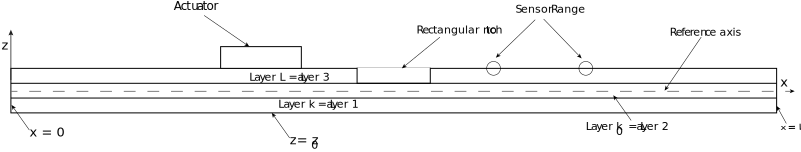
\includegraphics[width=\textwidth]{beamgeometry.png}
\caption{Beam Setup For The Experiment}
\label{fig:autoencoder_architecture}
\end{figure}

Notch positioning spans the central region of the beam structure, with center coordinates ranging from $x_{\text{notch}} = 1.6545$ meters to $x_{\text{notch}} = 1.8355$ meters. This positioning strategy ensures sufficient separation from boundary effects while maintaining adequate sensor coverage for response measurement. The notch depth parameter varies systematically from $d_{\text{notch}} = 0.0001$ meters to $d_{\text{notch}} = 0.001$ meters, corresponding to depth-to-height ratios ranging from approximately $6.7\%$ to $66.7\%$ of the total beam thickness. Notch width variations extend from $w_{\text{notch}} = 0.0001$ meters to $w_{\text{notch}} = 0.0012$ meters, encompassing narrow crack-like defects to more substantial geometric discontinuities.

A single sensor is repositioned across eleven predefined locations along the beam to capture wave propagation and scattering characteristics. Sensor locations are varied at coordinates
\[
x_{\text{sensor}} = [1.85, 1.87, 1.9, 1.92, 1.95, 1.97, 2.0, 2.02, 2.05, 2.1] \, \text{meters},
\]
providing comprehensive coverage of the post-notch region where scattered wave phenomena exhibit maximum sensitivity to damage parameters. This sensor distribution enables detailed characterization of wave transmission, reflection, and mode conversion effects that constitute the fundamental basis for damage detection and quantification methodologies.

The sensor measures the axial displacement response $u(x_{\text{sensor}}, z, t)$ at a fixed through-thickness coordinate $z = 0.00075$ meters, corresponding to the mid-plane location. This measurement strategy captures the primary wave propagation modes while avoiding complications associated with surface effects and boundary layer phenomena. The temporal response duration extends to $300$ microseconds with sampling rates sufficient to resolve wave propagation characteristics across the frequency range of interest.

\section{Low-Fidelity Dataset Generation Methodology}

The low-fidelity dataset generation employs one-dimensional zigzag beam theory implementations to create extensive training and validation datasets with computational efficiency advantages over high-fidelity approaches. Latin Hypercube Sampling (LHS) serves as the primary sampling strategy, providing superior space-filling properties compared to traditional random sampling approaches while ensuring comprehensive parameter space coverage.

The LHS implementation generates samples across three-dimensional parameter spaces encompassing notch location, depth, and width characteristics. Training dataset generation utilizes $750$  damage configurations sampled from the specified parameter bounds, representing a substantial increase over high-fidelity dataset sizes to compensate for the reduced model complexity. Testing dataset configurations include $100$ damage cases, maintaining appropriate proportions for robust model validation while ensuring computational tractability.

Material property variations introduce controlled complexity through systematic perturbations of baseline aluminum characteristics. The majority of configurations (approximately $85\%$) utilize nominal material properties with minor variations ($\pm 0.5\%$) to represent manufacturing tolerances and measurement uncertainties. The remaining configurations incorporate broader material property ranges, with density variations spanning $2650$-$2750$ kg/m$^3$ and elastic modulus variations ranging from $6.8 \times 10^{10}$ to $7.2 \times 10^{10}$ Pa.

Pristine beam configurations without notch damage comprise approximately $2.5\%$ of each dataset, providing baseline responses essential for damage detection algorithm development. These configurations uses varying material and geometric properties while setting notch parameters to zero, enabling direct comparison between damaged and undamaged structural responses.



The complete low-fidelity dataset encompasses $750$ primary damage training cases including material property variants and pristine configurations. Testing datasets maintain similar proportions with $100$ primary damage cases with corresponding variants. The total low-fidelity dataset comprises  $850$ simulation cases.

\section{High-Fidelity Dataset Generation Methodology}

The high-fidelity dataset generation process employs two-dimensional finite element method implementations to establish reference solutions with exceptional accuracy for comparative analysis and surrogate model validation. The reduced dataset size reflects the substantial computational requirements associated with full two-dimensional elasticity solutions while maintaining adequate statistical representation for model training purposes.

Training dataset generation utilizes $100$ carefully selected damage configurations sampled through LHS methodology, ensuring optimal parameter space coverage despite the constrained sample size. Testing dataset configurations include $50$  damage cases, providing sufficient validation data while managing computational resource allocation effectively. The parameter bounds remain identical to low-fidelity implementations, ensuring direct comparability between modeling approaches.

\begin{figure}[htbp]
\centering
\includegraphics[width=\textwidth]{parameters.png}
\caption{Notch Parameter sampling and their distribution for High Fidelity simulations}
\label{fig:parameters}
\end{figure}

Material property variations follow identical protocols to low-fidelity datasets, with $85\%$ of configurations utilizing nominal properties with minor variations and $15\%$ incorporating broader material property ranges. Pristine covers $1.5\%$ proportion, providing essential baseline comparisons across both fidelity levels.


\begin{figure}[htbp]
\centering
\includegraphics[width=\textwidth]{comparison_plot_pristine.png}
\caption{Comparison of 1D zigzag theory and 2D FEM responses for pristine beam configuration showing excellent agreement in displacement fields and stress distributions}
\label{fig:pristine_comparison}
\end{figure}

\begin{figure}[htbp]
\centering
\includegraphics[width=\textwidth]{comparison_plot1Dvs2D.png}
\caption{Comparative analysis of 1D zigzag theory versus 2D FEM responses for notched beam configurations highlighting correlation patterns and discrepancies across damage scenarios}
\label{fig:damage_comparison}
\end{figure}

The validation comparisons presented in Figures \ref{fig:pristine_comparison} and \ref{fig:damage_comparison} establish the fundamental relationship between one-dimensional zigzag theory predictions and two-dimensional finite element solutions. For the pristine beam configuration (Figure \ref{fig:pristine_comparison}), the 1D zigzag theory demonstrates substantial alignment with 2D FEM reference solutions across all sensor locations and time instances. This agreement validates the application of zigzag kinematics to homogeneous beam structures and confirms that the fictitious layering approach effectively captures the essential displacement field characteristics without introducing spurious artifacts.

The comparison for notched beam configurations (Figure \ref{fig:damage_comparison}) presents time-series response data from a single sensor location, revealing three distinct wave propagation modes that emerge due to the presence of the notch. The analysis demonstrates varying levels of agreement between 1D zigzag theory and 2D FEM solutions across different wave modes, providing critical insights into the capabilities and limitations of the reduced-order modeling approach.

The symmetric wave mode and the crack-induced wave mode exhibit strong correlation between 1D and 2D predictions, with primarily amplitude mismatches that remain within acceptable engineering tolerances for a low fidelity system. This alignment indicates that the zigzag theory effectively captures the global bending behavior and the primary scattering effects caused by the geometric discontinuity. The amplitude differences for these modes can be attributed to the simplified kinematic assumptions in the 1D formulation, which nevertheless preserve the essential wave propagation characteristics and energy distribution patterns.

However, the antisymmetric wave mode demonstrates significant deviation from the 2D FEM reference solution, unlike the pristine beam case where all modes showed better alignment. This discrepancy is particularly noteworthy as it suggests that the zigzag theory struggles to accurately capture certain higher-order deformation patterns that become prominent in the presence of damage. The antisymmetric mode, which involves complex shear deformation and through-thickness warping effects, appears to be inadequately represented by the fictitious layering approach employed in the 1D formulation. 

These mode-dependent discrepancies provide crucial justification for the multi-fidelity modeling approach adopted in this research. The 1D zigzag theory serves as an effective low-fidelity model that captures the essential physics of the dominant wave modes with reasonable computational efficiency, particularly for global response characteristics and primary damage signatures. However, the systematic deviations observed in the antisymmetric mode highlight the inherent limitations of the reduced-order approach in capturing complex two-dimensional stress fields and higher-order wave phenomena that develop around geometric discontinuities.

The 2D FEM approach, while computationally expensive, provides comprehensive resolution of all wave modes including the complex antisymmetric behavior that the 1D theory fails to capture accurately. This complementary relationship between the two approaches enables the transfer learning strategy employed in the multi-fidelity surrogate model, where the efficient 1D predictions provide rapid exploration of the parameter space while limited 2D data supplies the necessary corrective information to achieve high-fidelity accuracy across all wave propagation phenomena. 

\section{Computational Performance Analysis}

The computational requirements for dataset generation reveal substantial differences between low-fidelity and high-fidelity modeling approaches, directly impacting the feasibility of extensive parameter studies and real-time applications. Individual simulation times demonstrate the fundamental trade-off between model complexity and computational efficiency.

Low-fidelity simulations based on the one-dimensional zigzag beam theory require approximately $25$-$30s$ for the time integration phase and about \(45\,\text{s}\) in total per case on standard computational hardware. This efficiency arises from the substantially reduced degrees of freedom inherent in one-dimensional formulations and the absence of computationally expensive two-dimensional mesh generation and element assembly procedures. The total computational time for the complete low-fidelity dataset, comprising approximately \(850\) cases, amounts to roughly \(38{,}250\,\text{s}\), equivalent to about \(10.6\,\text{hours}\) of continuous computation.

\bigskip

In contrast, high-fidelity simulations employing two-dimensional finite element formulations demand significantly greater computational resources. The time integration stage alone requires approximately \(1700\text- 2000\,\text{s}\) (28.3-33.3 minutes) per case, while mesh generation, stiffness and mass matrix assembly, and related preprocessing steps add an additional \(6\,\text{minutes}\) per simulation. Consequently, the total computational time for the complete high-fidelity dataset of approximately \(150\) cases is around \(300{,}000\,\text{s}\) (\(83.3\,\text{hours}\)) or roughly 3.5 days, underscoring the considerable disparity in computational cost between the two fidelity levels.


The computational efficiency comparison reveals that one-dimensional zigzag implementations execute approximately $8$ times faster than equivalent two-dimensional finite element solutions while generating datasets nearly $8$ times larger. This performance differential demonstrates the fundamental advantage of reduced-order modeling approaches for extensive parameter studies and highlights the motivation for multi-fidelity surrogate modeling strategies that leverage both computational efficiency and solution accuracy.




% Chapter 4: Methodology
\chapter{Training and Evaluation Methodology}
\label{chap:methodology}



\section{Forward Problem: Model Architecture and Training}
\label{sec:forward_problem}

\subsection{Autoencoder Architecture and Training}

The autoencoder component serves as the foundational element of the surrogate modeling framework, providing dimensionality reduction capabilities that transform high-dimensional time-series response data into compact latent representations suitable for subsequent machine learning operations. This architectural choice enables efficient parameter-to-response mapping by decoupling the representation learning problem from the regression task, thereby facilitating multi-fidelity fusion strategies and improving computational tractability.

\subsubsection{Architecture Design Rationale}

The autoencoder architecture employs a response-only training paradigm where the encoder-decoder system learns compression mappings exclusively from structural response data. This approach leverages a fundamental insight: damage-induced response characteristics possess intrinsic geometric structure that manifests consistently across the response space, independent of the underlying parameter configurations that produced them. By feeding only response signals through the compression pathway, the latent space self-organizes according to pure structural response features: wave propagation characteristics, frequency content, amplitude modulations, and damage signatures, creating a representation that captures the essential physics of structural behavior.
This response-centric design delivers substantial benefits for multi-fidelity surrogate modeling. The learned latent representations remain directly interpretable as structural response phenomena rather than abstract parameter-response amalgamations, enabling physically meaningful analysis of the compression. The architecture naturally facilitates transfer learning between fidelity levels, as responses exhibiting similar damage signatures converge to neighboring latent regions regardless of whether they originate from low-fidelity or high-fidelity models, effectively bridging modeling discrepancies through shared response patterns. Furthermore, the separation between compression and regression enables independent optimization: the autoencoder focuses purely on maximizing reconstruction fidelity while subsequent regression networks map latent codes to parameters without architectural compromises.
An alternative parameter-conditional architecture, where both responses and parameters feed into the encoder, proves less effective for this application. Such designs force the latent space to simultaneously encode parameter information and response characteristics, creating entangled representations where gradient signals for reconstruction compete with those for parameter prediction. The resulting latent codes lose their interpretability as pure response features, instead memorizing parameter-response correlations that may not generalize across fidelity levels. Moreover, parameter conditioning introduces gradient conflicts during end-to-end training, as the network must balance reconstruction accuracy against parameter prediction, ultimately degrading performance on both objectives compared to the staged approach enabled by response-only compression.

\begin{figure}[htbp]
\centering
\includegraphics[width=\textwidth]{AEII.png}
\caption{Autoencoder Architecture from the experiment}
\label{fig:autoencoder_architecture}
\end{figure}

\subsection{Encoder Network Architecture}
\label{subsec:encoder_architecture}

The encoder network implements a progressive dimensionality reduction pathway, transforming input time-series data of dimension $1500$ into a compact $30$-dimensional latent representation through a sequence of fully connected layers with strategic regularization mechanisms. The encoder comprises four linear transformation layers with monotonically decreasing hidden dimensions:
\[
1500 \rightarrow 1024 \rightarrow 512 \rightarrow 256 \rightarrow 30.
\]
This gradual compression strategy avoids abrupt information bottlenecks that can destabilize training dynamics and degrade reconstruction quality.

Each hidden layer incorporates batch normalization immediately following the linear transformation, providing adaptive input rescaling that accelerates convergence and mitigates internal covariate shift during training. Batch normalization parameters $-$ learned scale and shift coefficients $-$ enable the network to automatically adjust feature distributions across layers, reducing sensitivity to initialization schemes and learning rate selection.

Leaky rectified linear unit (LeakyReLU) activation functions with negative slope $\alpha = 0.2$ introduce controlled nonlinearity while preserving gradient flow through negative input regions. This activation choice addresses the ``dying ReLU'' phenomenon, wherein standard ReLU units producing consistently negative pre-activations cease to learn due to zero gradients. The non-zero negative slope ensures that all encoder neurons maintain learning capacity throughout training, particularly important for capturing subtle damage signatures that may manifest as small-amplitude response perturbations.

\begin{figure}[htbp]
\centering
\includegraphics[width=\textwidth]{leakyrelu.png}
\caption{Leaky ReLU
with coefficient 0.2}
\label{fig:leakyrelu}
\end{figure}

Dropout regularization with probability $p = 0.1$ appears after each activation function, stochastically deactivating 10\% of neurons during training passes. This technique enforces redundant encoding strategies, preventing the network from relying exclusively on specific neuron combinations and improving generalization to unseen response patterns. The relatively conservative dropout rate balances regularization benefits against the risk of underfitting, acknowledging that the primary dataset contains limited high-fidelity samples requiring careful capacity management.

The final encoder layer projects the $256$-dimensional penultimate representation into the $30$-dimensional latent space without subsequent activation or normalization, allowing the latent coordinates to assume arbitrary real values. This unrestricted latent space facilitates linear interpolation between response patterns and supports the subsequent gradient-based parameter identification procedures.

\paragraph{Performance Comparison.}
A comparative evaluation revealed that the fully connected MLP-based encoder–decoder achieved superior latent representation accuracy, with a latent space coefficient of determination $R^2_{\text{latent}} = 0.9243$, compared to $R^2_{\text{latent}} = 0.8997$ for the 1D convolutional encoder–decoder. Despite exhibiting similar reconstruction $R^2$ for the overall time-series outputs, the CNN-based approach demonstrated a weaker latent embedding fidelity, indicating that convolutional feature extraction provided limited benefit for globally correlated, non-stationary vibration responses. In contrast, the MLP’s dense connectivity allowed more effective compression of distributed temporal dependencies, yielding a more expressive latent encoding.


\subsubsection{Latent Space Dimensionality Selection}


The latent space dimensionality of 30 represents a carefully balanced compromise between representational capacity and regression complexity. Dimensionality selection constitutes a critical hyperparameter directly impacting both reconstruction accuracy and downstream machine learning performance. Insufficient latent dimensions produce information bottlenecks that destroy essential response characteristics required for accurate damage characterization, while excessive dimensions unnecessarily complicate the parameter-to-latent regression problem and increase susceptibility to overfitting.


Preliminary dimensionality experiments revealed that latent spaces below 20 dimensions exhibit systematic reconstruction errors exceeding acceptable thresholds, particularly for high-severity damage cases characterized by complex nonlinear response modifications. Conversely, latent dimensions exceeding 40 demonstrate only marginal reconstruction improvements while moderately degrading XGBoost regression accuracy due to the curse of dimensionality—the exponential increase in sample requirements for adequate representation of high-dimensional spaces.


Complementary to these observations, Proper Orthogonal Decomposition (POD) analysis of the response dataset indicated that the first 30 modes capture over \text{99\%} of the total energy content, suggesting that this dimensionality suffices to represent the dominant spatiotemporal response features without significant information loss. This empirical finding reinforces the autoencoder-based selection, confirming that a 30-dimensional latent space effectively encapsulates the essential dynamic signatures of the structure.


The chosen 30-dimensional latent space achieves near-perfect reconstruction of training responses (Reconstruction $R^{2}$ around $0.99$) while maintaining tractable regression complexity for the available training sample sizes. This dimensionality captures dominant response modes corresponding to fundamental beam vibration characteristics, damage-induced frequency shifts, and amplitude modulation patterns, as evidenced by latent space visualization studies demonstrating smooth, continuous organization of response trajectories according to damage severity and location.


\subsection{Decoder Network Architecture}
\label{subsec:decoder_architecture}

The decoder implements an expansion pathway that maps latent vectors in $\mathbb{R}^{30}$ back to full-resolution time-series responses in $\mathbb{R}^{1500}$. Its dimensional progression mirrors the encoder only in spirit (coarse-to-fine), but is deliberately asymmetric in depth to avoid over-parameterizing the reconstruction stage:
\[
30 \;\rightarrow\; 512 \;\rightarrow\; 1024 \;\rightarrow\; 1500.
\]
This choice reflects a pragmatic assumption: once salient structure has been compacted into a low-dimensional representation, a modest number of expressive layers suffices to reconstitute high-dimensional outputs without incurring unnecessary capacity or training instability.

Each hidden block applies a linear transformation followed by batch normalization and a LeakyReLU nonlinearity with negative slope $\alpha=0.2$. Batch normalization stabilizes layer-wise signal scales during training and reduces sensitivity to optimizer hyperparameters, while LeakyReLU preserves gradient flow through negative pre-activations and avoids the ``dying ReLU'' failure mode during reconstruction.

The decoder  employ dropout with probability $p=0.2$ after each hidden activation. This regularization targets co-adaptation among decoder features and improves robustness of the reconstruction mapping from latent space. Importantly, stochasticity from dropout is confined to \texttt{train} mode; during evaluation/inference (\texttt{eval} mode) dropout is disabled, yielding deterministic outputs for a fixed latent vector~$\mathbf{z}$. Hence, the use of decoder dropout does \emph{not} compromise determinism required for surrogate modeling or parameter identification.

The output layer is strictly linear:
\begin{equation}
    \mathbf{\hat{x}} = W_3\,\phi_2\!\bigl(W_2\,\phi_1(W_1\,\mathbf{z})\bigr) + \mathbf{b}_3,
\end{equation}

where $W_1 \in \mathbb{R}^{512 \times 30}$, $W_2 \in \mathbb{R}^{1024 \times 512}$, $W_3 \in \mathbb{R}^{1500 \times 1024}$, $\mathbf{b}_3 \in \mathbb{R}^{1500}$, and $\phi_i(\cdot)$ denote the BatchNorm\,$\circ$\,LeakyReLU\,$\circ$\,Dropout blocks with $p=0.2$. The absence of a bounded activation (e.g., sigmoid, $\tanh$) at the output permits the model to reproduce the full dynamic range of target responses without saturation. If application constraints mandate range bounding, a post-hoc affine rescaling with a bounded head can be introduced, but this is unnecessary for the present regression setting and can harm gradient signal near extrema.

Overall, the decoder trades strict architectural symmetry for a capacity profile that is sufficient but not excessive: two expressive hidden layers (512 and 1024 units) regularized by batch normalization and dropout, followed by a linear projection to the $1500$-dimensional signal space. This configuration has proven stable in training and yields high-fidelity reconstructions when paired with the progressive, regularized encoder in Section~\ref{subsec:encoder_architecture}.


\subsubsection{Loss Function Formulation}
The autoencoder training objective employs the mean squared error (MSE) loss function as its primary reconstruction criterion, measuring time-step–wise discrepancies between the input and reconstructed time-series responses. The loss is formally expressed as
\[
\mathcal{L}_{\text{MSE}}
= \frac{1}{N \cdot T}
\sum_{i=1}^{N}
\sum_{t=1}^{T}
\left( x_i(t) - \hat{x}_i(t) \right)^2,
\]
where $N$ denotes the batch size, $T = 1500$ represents the time-series length, $x_i(t)$ is the ground-truth response of the $i^{\text{th}}$ sample at time step $t$, and $\hat{x}_i(t)$ denotes its autoencoder reconstruction. The MSE loss naturally arises as the negative log-likelihood under an independent Gaussian noise assumption, corresponding to maximum likelihood estimation of the reconstruction parameters.

To improve generalization, Gaussian noise with a small standard deviation ($\sigma = 0.03$) is added to the training responses, effectively implementing data augmentation without altering the underlying clean distribution. This regularization strategy encourages the model to learn smooth latent representations while remaining robust to minor perturbations.

During the multi-fidelity fine-tuning phase on high-fidelity (2D FEM) data, the reconstruction loss is further scaled by a weighting coefficient $\alpha = 3.0$ to emphasize accurate learning from the higher-fidelity domain:
\[
\mathcal{L}_{\text{MFSM}} = \alpha \, \mathcal{L}_{\text{MSE}}, \quad \text{with } \alpha = 3.0.
\]
This weighting scheme ensures that fine-tuning gradients arising from the high-fidelity dataset receive proportionally greater influence relative to those from the low-fidelity pretraining phase.

In addition, a small $L_2$ regularization term (implemented via the Adam optimizer’s \texttt{weight\_decay} parameter) is applied to network parameters $\Theta$ to prevent overfitting:
\[
\mathcal{L}_{\text{total}}
= \mathcal{L}_{\text{MFSM}}
+ \lambda \sum_{p \in \Theta} \| p \|_2^2,
\quad \lambda = 10^{-5}.
\]
The combined objective thus penalizes large reconstruction errors and excessively large parameter magnitudes, promoting stable and smooth convergence.

From a statistical perspective, the quadratic penalty inherent to MSE enforces a strong bias toward minimizing large deviations, compelling the autoencoder to accurately reconstruct dominant structural response features rather than focusing on minor fluctuations. Given that the employed datasets originate from controlled numerical simulations and contain no measurement outliers, alternative formulations such as the mean absolute error (MAE) or hybrid MSE–MAE losses offered no measurable advantage during preliminary testing. Consequently, the pure MSE objective, augmented with Gaussian noise regularization and mild $L_2$ weight decay, was adopted as the final reconstruction criterion for both pretraining and fine-tuning stages.

\subsubsection{Optimization Algorithm and Learning Rate Strategy}

Model training employs the Adam (Adaptive Moment Estimation) optimizer, a first-order gradient-based optimization algorithm combining momentum and adaptive learning rate mechanisms. Adam maintains exponential moving averages of both gradients and squared gradients, enabling efficient navigation of complex loss landscapes characteristic of deep neural networks.

For low-fidelity surrogate model (LFSM) training on one-dimensional zigzag response data, the learning rate is set to $\eta = 1 \times 10^{-4}$, balancing convergence speed against training stability. This moderately conservative learning rate accommodates the relatively large training dataset (750 cases) and the encoder's substantial depth (four hidden layers), ensuring stable gradient updates throughout training.

Multi-fidelity surrogate model (MFSM) fine-tuning adopts a reduced learning rate of $\eta = 1 \times 10^{-5}$, reflecting the transfer learning context where the autoencoder initializes from pre-trained LFSM weights. The order-of-magnitude learning rate reduction prevents catastrophic forgetting of low-fidelity response representations while enabling gradual adaptation to high-fidelity response characteristics. This conservative fine-tuning strategy proves essential given the limited high-fidelity dataset (approximately 100 training samples), where aggressive learning rates risk overfitting to the small sample of two-dimensional finite element responses.

Weight decay regularization with coefficient $\lambda = 1 \times 10^{-5}$ supplements the optimization objective, penalizing large parameter magnitudes through L2 regularization:
\[
\mathcal{L}_{\text{total}} = \mathcal{L}_{\text{MSE}} + \lambda \sum_{l} \|\mathbf{W}_l\|_2^2
\]
where $\mathbf{W}_l$ represents weight matrices across all layers. Weight decay discourages complex, high-magnitude weight configurations, promoting simpler models that generalize better to unseen data—particularly valuable for the MFSM scenario where limited high-fidelity samples heighten overfitting risks.

No explicit learning rate scheduling strategies are employed; the learning rate remains constant throughout training. Preliminary experiments with common scheduling approaches—including exponential decay, step decay, and cosine annealing—yielded negligible performance differences for the present autoencoder architecture and dataset sizes, suggesting that fixed learning rates suffice when combined with early stopping procedures (discussed below).

\subsubsection{Regularization Techniques}

Beyond dropout and weight decay previously discussed, the training protocol incorporates several additional regularization mechanisms ensuring robust generalization performance.

Early stopping monitors validation set reconstruction loss, terminating training when validation performance ceases to improve for a specified patience period. The patience parameter is set to 30 epochs, allowing training to continue through temporary validation loss plateaus while preventing excessive overfitting when genuine convergence occurs. Early stopping effectively implements implicit regularization by selecting model checkpoints corresponding to optimal validation performance, avoiding the overfitting that inevitably arises from unconstrained training duration.

The early stopping mechanism maintains a running record of validation losses, identifying the epoch yielding minimum validation error. Training terminates when 30 consecutive epochs fail to surpass the best recorded validation performance, at which point the model checkpoint corresponding to the optimal validation epoch is restored as the final trained model. This procedure ensures that the deployed autoencoder represents the best-generalizing configuration encountered during training, rather than the potentially overfitted final epoch weights.

Batch normalization provides a subtler form of regularization beyond its primary role in stabilizing training dynamics. By computing normalization statistics over mini-batches during training, batch normalization introduces stochastic noise dependent on batch composition—effectively performing a form of implicit data augmentation. During inference, batch statistics are replaced by running averages accumulated during training, ensuring deterministic predictions while retaining the regularization benefits imparted during the training phase.

The combination of dropout, weight decay, batch normalization, and early stopping constitutes a comprehensive regularization suite addressing multiple failure modes. Dropout and weight decay explicitly constrain model capacity, batch normalization stabilizes training and provides implicit augmentation, and early stopping prevents temporal overfitting through judicious training duration selection.

\subsubsection{Batch Size and Training Protocol}

Training batch sizes differ between LFSM and MFSM training phases, reflecting their distinct dataset sizes and optimization requirements. LFSM training utilizes batch size 64, providing stable gradient estimates while maintaining computational efficiency through GPU-accelerated batch-parallel processing. The relatively large batch size exploits the substantial low-fidelity training dataset, enabling the batch normalization statistics to accurately represent data distributions and producing gradient estimates with low variance.

MFSM fine-tuning employs reduced batch size 32, acknowledging the limited high-fidelity training data. Smaller batches increase gradient variance, introducing beneficial noise that can help escape suboptimal local minima during fine-tuning. Additionally, the reduced batch size ensures that batch normalization statistics derive from sufficiently diverse samples despite the constrained dataset, avoiding the pathological behavior that can occur when batch size approaches dataset size.

Training proceeds for maximum epoch counts of 200 (LFSM) and 100 (MFSM), though early stopping typically terminates training substantially earlier. One epoch constitutes a complete pass through the training dataset, with data randomly shuffled before each epoch to decorrelate consecutive mini-batches and reduce the impact of sample ordering on convergence dynamics.

During each training iteration, a mini-batch of time-series responses is drawn from the training set, forward-propagated through the autoencoder to produce reconstructions and latent representations, and compared against the original inputs via the MSE loss function. Backpropagation computes loss gradients with respect to all trainable parameters (encoder and decoder weights and biases, batch normalization parameters), which are then used to update parameters via the Adam optimizer. Training data undergoes augmentation through stochastic dropout mask sampling, while validation data passes through the network deterministically with dropout disabled.

Table~\ref{tab:ae_hyperparameters} summarizes the key hyperparameters employed for autoencoder training in both the Low-Fidelity Surrogate Model (LFSM) and Multi-Fidelity Surrogate Model (MFSM) configurations.

\begin{table}[htbp]
\centering
\caption{Autoencoder hyperparameters for LFSM and MFSM training}
\label{tab:ae_hyperparameters}
\begin{tabular}{lcc}
\hline
\textbf{Hyperparameter} & \textbf{LFSM} & \textbf{MFSM} \\
\hline
Input Dimension & 1500 & 1500 \\
Latent Dimension & 30 & 30 \\
Encoder Architecture & 1500$\rightarrow$1024$\rightarrow$512$\rightarrow$256$\rightarrow$30 & 1500$\rightarrow$1024$\rightarrow$512$\rightarrow$256$\rightarrow$30 \\
Decoder Architecture & 30$\rightarrow$512$\rightarrow$1024$\rightarrow$1500 & 30$\rightarrow$512$\rightarrow$1024$\rightarrow$1500 \\
Activation Function & LeakyReLU ($\alpha=0.2$) & LeakyReLU ($\alpha=0.2$) \\
Encoder Dropout & 0.1 & 0.1 \\
Decoder Dropout & 0.2 & 0.2 \\
Batch Normalization & Yes & Yes \\
Optimizer & Adam & Adam \\
Learning Rate ($\eta$) & $1 \times 10^{-4}$ & $1 \times 10^{-5}$ \\
Weight Decay ($\lambda$) & $1 \times 10^{-5}$ & $1 \times 10^{-5}$ \\
Loss Function & MSE & Weighted MSE ($\alpha=3.0$) \\
Batch Size & 64 & 32 \\
Maximum Epochs & 200 & 100 \\
Early Stopping Patience & 30 & 30 \\
Noise Augmentation ($\sigma$) & 0.03 & 0.03 \\
Training Dataset Size & 750 cases & 100 cases (+ pretrained) \\
\hline
\end{tabular}
\end{table}

The primary differences between LFSM and MFSM configurations lie in the learning rate (reduced 10-fold for fine-tuning), batch size (halved to accommodate smaller dataset), maximum training epochs (halved due to transfer learning initialization), and loss function weighting (3× emphasis on high-fidelity reconstruction). The architectural components remain identical to preserve learned feature representations during multi-fidelity transfer.



\subsection{XGBoost Configuration and Training}

The XGBoost (Extreme Gradient Boosting) component establishes the parameter-to-latent space mapping, enabling direct prediction of autoencoder latent representations from notch damage parameters. This gradient boosting framework constructs an ensemble of decision trees through iterative refinement, wherein each successive tree corrects residual errors from preceding trees. The combination of autoencoder-learned latent representations with XGBoost regression decouples the nonlinear response compression problem from the parameter mapping task, facilitating efficient surrogate model construction through specialized component optimization.

\subsubsection{Model Architecture and Regression Strategy}

XGBoost implements multi-output regression to map six-dimensional parameter vectors to 30-dimensional latent space coordinates. The input parameters comprise: notch location ($x_{\text{notch}}$), notch depth ($d_{\text{notch}}$), notch width ($w_{\text{notch}}$), elastic modulus ($E$), density ($\rho$), and response measurement location ($\ell$). The XGBRegressor automatically handles multi-output targets by internally maintaining separate leaf values for each output dimension while sharing the tree structure, effectively training 30 coordinated models that learn common feature interactions while maintaining output-specific predictions.

This multi-output strategy exploits the statistical independence assumption among latent dimensions, hypothesizing that individual latent coordinates capture distinct response features (e.g., amplitude, frequency content, phase characteristics) that can be independently predicted from damage parameters. The shared tree structure across outputs ensures computational efficiency, as split point determination occurs once per feature while leaf value optimization proceeds independently for each latent dimension.

The parameter-to-latent mapping approach offers significant advantages over direct parameter-to-response regression. First, the 30-dimensional latent space exhibits substantially lower dimensionality than the 1500-point time-series responses, reducing regression complexity and sample requirements by approximately 98\%. Second, the autoencoder pre-training establishes smooth latent space geometry where nearby parameter configurations produce proximate latent representations, improving the interpolation behavior of tree-based regressors. Third, the modular architecture enables independent optimization of compression quality (autoencoder) and mapping accuracy (XGBoost), avoiding the training difficulties inherent in end-to-end deep learning approaches for limited-data scenarios.

\subsubsection{Hyperparameter Selection Methodology}

Hyperparameter selection balances model capacity against overfitting risks through careful consideration of dataset characteristics, computational constraints, and generalization requirements. The selected configuration reflects empirical optimization informed by preliminary grid search experiments and theoretical understanding of gradient boosting behavior.

\paragraph{Number of Estimators (Trees)} 
The ensemble comprises $n_{\text{estimators}} = 2000$ trees, providing substantial model capacity for capturing complex nonlinear parameter-latent relationships while leveraging the boosting framework's inherent regularization. Each tree fits residuals from preceding trees, mitigating overfitting despite the large ensemble size when combined with appropriate learning rate selection and early stopping. Preliminary experiments reveal performance saturation beyond 1500--2000 estimators, indicating marginal accuracy improvements from additional trees. The selected value balances asymptotic performance against computational costs and memory footprint.

\paragraph{Maximum Tree Depth} 
Individual tree depth is constrained to $d_{\text{max}} = 10$ levels, limiting feature interaction complexity within single trees while capturing high-order multi-way interactions. This moderate depth controls the bias-variance trade-off: shallow trees exhibit high bias but low variance, while deep trees demonstrate low bias but high variance and severe overfitting. The depth-10 configuration resides in a favorable intermediate regime, capturing essential nonlinear relationships without pathological overfitting characteristic of unrestricted trees. This depth also reflects the underlying physics: notch response depends on complex interactions among damage parameters (location, geometry) and structural properties (dimensions, material), suggesting that intermediate trees capturing three- to four-way feature interactions suffice for accurate representation.

\paragraph{Learning Rate (Shrinkage)} 
The learning rate $\eta = 0.02$ applies multiplicative shrinkage to each tree's contribution, attenuating individual predictions to promote ensemble diversity and prevent premature convergence. This conservative rate necessitates larger ensemble sizes but produces smoother, more robust models less susceptible to outliers. Combined with $n_{\text{estimators}} = 2000$, this configuration approximates the effective capacity of $\eta = 0.1$ with 400 trees while demonstrating enhanced generalization in cross-validation. The choice reflects the constrained high-fidelity dataset ($\approx$100 training cases), where aggressive learning rates risk fitting noise rather than genuine physical patterns.

\paragraph{Subsample and Column Sampling} 
Stochastic gradient boosting with $s = 0.8$ subsample ratio randomly selects 80\% of training samples per tree, introducing controlled randomness that enhances ensemble diversity and reduces overfitting through decorrelated predictions. This row-sampling strategy provides computational benefits ($\approx$20\% speedup) while acting as a regularizer analogous to bootstrap aggregating. Feature subsampling with $c = 0.8$ column sampling ratio randomly selects 80\% of input features per tree, complementing row subsampling to further decorrelate ensemble members. Each tree observes a random subset of the six input parameters, preventing feature dominance and improving robustness to irrelevant or redundant predictors. The 80\% fractions balance diversity benefits against statistical efficiency losses from discarded data.

\paragraph{Gradient-based Sampling Strategy} 
Gradient-based sampling preferentially selects training instances according to gradient magnitudes, focusing computational effort on difficult-to-predict samples exhibiting large residual errors. This adaptive strategy allocates tree capacity toward correcting systematic prediction failures rather than refining already-accurate predictions, improving worst-case performance and reducing maximum errors. For the present application, high-severity damage cases (deep, wide notches) produce complex nonlinear responses more challenging to predict than pristine configurations. Gradient-based sampling ensures adequate model capacity allocation to these difficult instances, preventing the model from sacrificing accuracy on challenging parameter regions.



\subsubsection{Convergence Monitoring and Model Persistence}

XGBoost training employs iterative boosting with early stopping capability based on validation set performance. While the present implementation uses fixed ensemble sizes (2000 estimators) determined through preliminary experimentation, the training framework supports early stopping that would monitor validation loss after each boosting iteration, terminating training when performance ceases to improve for a specified number of consecutive iterations. The conservative learning rate ($\eta = 0.02$) and moderate tree depth (10 levels) selected here produce stable convergence behavior that reliably reaches optimal performance within 2000 iterations.

Training convergence is assessed through latent space prediction accuracy metrics computed on held-out validation data. Training set $R^2$ coefficients quantify in-sample fit quality, while validation set $R^2$ evaluates generalization to unseen parameter configurations. Successful training exhibits high validation $R^2$ (typically $> 0.90$) with minimal training-validation gaps ($< 0.05$), indicating that the model captures genuine parameter-latent relationships rather than memorizing training-specific noise.

Trained XGBoost models are persisted to disk using joblib serialization, preserving the complete ensemble structure including all tree parameters, feature importance statistics, and training metadata. Model serialization facilitates rapid deployment for inverse problem solving and forward prediction tasks without retraining overhead, while also enabling reproducible research through standardized model checkpointing.

Table~\ref{tab:xgb_hyperparameters} summarizes the key hyperparameters employed for XGBoost training across all surrogate model configurations (LFSM, MFSM, and HFSM). The XGBoost component maintains identical hyperparameters across all fidelity levels, as it operates exclusively on latent space representations rather than raw response data.

\begin{table}[htbp]
\centering
\caption{XGBoost hyperparameters for all surrogate models}
\label{tab:xgb_hyperparameters}
\begin{tabular}{lc}
\hline
\textbf{Hyperparameter} & \textbf{Value} \\
\hline
Input Dimension & 6 \\
Output Dimension (Latent) & 30 \\
Number of Estimators & 2000 \\
Maximum Tree Depth & 10 \\
Learning Rate ($\eta$) & 0.02 \\
Subsample Ratio & 0.8 \\
Column Sample Ratio & 0.8 \\
Sampling Method & Gradient-based \\
Tree Construction Method & \texttt{gpu\_hist} / \texttt{hist} \\
Objective Function & Regression (MSE) \\
Number of Feature Bins & 255 \\
GPU Acceleration & Enabled (if available) \\
Multi-output Strategy & Shared tree structure \\
Early Stopping & Supported \\
Model Persistence & Joblib serialization \\
\hline
\end{tabular}
\end{table}

Unlike the autoencoder component, which requires different learning rates and batch sizes between LFSM and MFSM training, the XGBoost regressor maintains uniform hyperparameters across all fidelity levels (LFSM, MFSM, and HFSM). This consistency reflects the fact that XGBoost operates on pre-computed latent representations extracted from the respective autoencoders, rather than directly processing time-series responses. The primary difference between models lies solely in the training dataset size ($\sim$750 cases for LFSM, $\sim$100 cases for MFSM and HFSM) and the source of latent vectors (LFSM encoder, MFSM fine-tuned encoder, or HFSM encoder).


\subsection{High-Fidelity Surrogate Model Architecture}

The high-fidelity surrogate model (HFSM) serves as a direct surrogate for 2D finite element analysis, employing an identical neural architecture to Stage 2 of the multi-fidelity framework. The model architecture consists of a non-conditional convolutional autoencoder paired with an XGBoost gradient boosting regressor for parameter-to-latent space mapping, maintaining consistency with the MFSM decoder training strategy.

Training data for HFSM derives exclusively from 2D FEM simulations, which provide higher-fidelity reference responses compared to 1D zigzag theory predictions but at significantly increased computational cost (approximately 5 minutes per case versus 40 seconds for 1D simulations). The training dataset comprises approximately 100 cases selected using Latin Hypercube Sampling (LHS) to ensure representative coverage across the parameter space of notch geometry (location, depth, width), material properties (elastic modulus, density), and sensor locations. With 11 sensor locations per case, this yields approximately 1100 training samples total. The LHS strategy provides near-uniform exploration of the six-dimensional parameter space while maintaining statistical efficiency, ensuring adequate representation of the full range of damage configurations and structural properties.

The autoencoder architecture mirrors the MFSM decoder specifications: a 30-dimensional latent space with progressive compression through layers [1500 → 1024 → 512 → 256 → 30] for encoding and symmetric expansion for decoding. Training employs identical hyperparameters to ensure fair comparison: batch size of 32, learning rate of $10^{-5}$, LeakyReLU activation with negative slope 0.2, batch normalization after each linear layer, and dropout regularization at 0. The training objective minimizes mean squared reconstruction error with early stopping based on a patience of 30 epochs.

XGBoost surrogate training follows the same configuration as MFSM, utilizing 2000 gradient boosting iterations with maximum tree depth of 10 and learning rate $\eta = 0.02$. The surrogate learns the mapping from scaled input parameters (normalized to $[-1, 1]$) to the 30-dimensional latent representation, with GPU acceleration enabled for histogram-based tree construction when hardware permits.

The HFSM provides a critical baseline for assessing multi-fidelity enhancement: by training exclusively on high-fidelity 2D data without leveraging low-fidelity priors, it quantifies the maximum achievable accuracy given limited high-fidelity samples. Comparative evaluation against MFSM (which combines 750 low-fidelity cases with 0 high-fidelity cases) isolates the value added by the multi-fidelity fusion strategy, demonstrating whether low-fidelity data augmentation can approach or exceed the performance of pure high-fidelity training with twice the 2D simulation budget.


\subsection{Forward Problem Evaluation Metrics}

The forward surrogate models (LFSM, HFSM, and MFSM) require comprehensive evaluation across multiple dimensions to assess both predictive accuracy and computational efficiency. The evaluation framework stratifies metrics into reconstruction quality measures and computational performance indicators, enabling quantitative comparisons across different fidelity levels and training strategies.

\subsubsection{Reconstruction Quality Metrics}

The primary assessment of surrogate model performance focuses on the fidelity of reconstructed time-series responses relative to ground truth data. The evaluation employs a comprehensive suite of global metrics to quantify prediction accuracy across multiple dimensions.

\paragraph{Coefficient of Determination (R²)} The R² metric quantifies the proportion of variance in the true response explained by the surrogate model predictions. For time-series data $\mathbf{y}_{\text{true}} \in \mathbb{R}^{N_t}$ and predictions $\mathbf{y}_{\text{pred}} \in \mathbb{R}^{N_t}$ where $N_t = 1500$ represents the temporal discretization:

\begin{equation}
R^2 = 1 - \frac{\sum_{i=1}^{N_t} (y_{\text{true},i} - y_{\text{pred},i})^2}{\sum_{i=1}^{N_t} (y_{\text{true},i} - \bar{y}_{\text{true}})^2}
\end{equation}

where $\bar{y}_{\text{true}}$ denotes the temporal mean of the true response. The R² statistic ranges from $-\infty$ to 1, with $R^2 = 1$ indicating perfect reconstruction, $R^2 = 0$ representing performance equivalent to naive mean prediction, and negative values signifying predictions worse than the mean baseline. Per-sample R² scores are also computed individually for each test case to assess prediction consistency and identify potential failure modes across different parameter configurations.

\paragraph{Mean Squared Error (MSE)} The MSE quantifies the average squared deviation between predicted and true responses:

\begin{equation}
\text{MSE} = \frac{1}{N_t} \sum_{i=1}^{N_t} (y_{\text{true},i} - y_{\text{pred},i})^2
\end{equation}

MSE penalizes large errors more heavily than small deviations due to the quadratic penalty, making it sensitive to outlier predictions. For multi-sample evaluation across $N_s$ test cases, the global MSE aggregates errors over all time-series:

\begin{equation}
\text{MSE}_{\text{global}} = \frac{1}{N_s \times N_t} \sum_{j=1}^{N_s} \sum_{i=1}^{N_t} (y_{\text{true},j,i} - y_{\text{pred},j,i})^2
\end{equation}



\paragraph{Normalized Mean Squared Error (NMSE)} To enable dimensionless comparisons across datasets with different response magnitudes, the NMSE normalizes MSE by the variance of the true signal:

\begin{equation}
\text{NMSE} = \frac{\text{MSE}}{\text{Var}(\mathbf{y}_{\text{true}})} = \frac{\sum_{i=1}^{N_t} (y_{\text{true},i} - y_{\text{pred},i})^2}{\sum_{i=1}^{N_t} (y_{\text{true},i} - \bar{y}_{\text{true}})^2}
\end{equation}

The NMSE relates directly to R² through $\text{NMSE} = 1 - R^2$. Expressing NMSE as a percentage $(\text{NMSE}\% = 100 \times \text{NMSE})$ provides an intuitive interpretation of the relative error magnitude.


\section{Inverse Problem Formulation}
\label{sec:inverse_problem}

\subsection{Problem Statement and Mathematical Framework}

The inverse problem addresses the practical challenge of structural health monitoring: estimating unknown notch characteristics from measured dynamic response data. While forward modeling predicts structural responses for known parameters (Section 4.1), the inverse problem reverses this relationship to identify damage from observed vibrations. This capability is crucial for automated structural inspection systems where direct visual inspection is impractical or cost-prohibitive.

\subsubsection{Inverse Problem Definition}
Mathematically, the inverse problem seeks to recover the optimal notch parameters $\boldsymbol{\theta}^*$ that minimize the discrepancy between predicted and observed responses:
\begin{equation}
\boldsymbol{\theta}^* = \arg\min_{\boldsymbol{\theta} \in \mathcal{D}} \mathcal{L}\left(\mathcal{F}_{\text{MFSM}}(\boldsymbol{\theta}), \mathbf{u}^{\text{obs}}\right)
\label{eq:inverse_optimization}
\end{equation}
where $\mathcal{F}_{\text{MFSM}}$ is the multi-fidelity surrogate forward model, $\mathcal{L}$ is the objective function defined in Section~\ref{sec:objective_function}, and $\mathcal{D}$ represents the feasible parameter domain.

The parameter vector for this study focuses on three geometric descriptors of rectangular notches:
\begin{equation}
\boldsymbol{\theta} = \begin{bmatrix}
x_{\text{notch}} \\ d_{\text{notch}} \\ w_{\text{notch}}
\end{bmatrix}, \quad
\begin{cases}
x_{\text{notch}} \in [1.6545, 1.8355] \text{ m} & \text{(location along beam)} \\
d_{\text{notch}} \in [0.0001, 0.001] \text{ m} & \text{(notch depth)} \\
w_{\text{notch}} \in [0.0001, 0.0012] \text{ m} & \text{(notch width)}
\end{cases}
\label{eq:parameter_bounds}
\end{equation}

The structural configuration assumes known beam properties: length $L = 3.0$ m, material density $\rho = 2700$ kg/m$^3$, Young's modulus $E = 7 \times 10^{10}$ Pa, with the sensor positioned at $x_{\text{obs}} = 1.9$ m for response acquisition.

\subsubsection{Challenges in Inverse Problem Solving}

\paragraph{Ill-Posedness and Regularization}
Inverse problems typically violate one or more of Hadamard's conditions for well-posedness:

\begin{enumerate}
    \item \textbf{Existence:} A solution exists only if the observed response lies within the forward model's achievable response space. Using 2D FEM responses as ground truth ensures theoretical existence, though measurement noise and sensor limitations may introduce practical violations.

    \item \textbf{Uniqueness:} The parameter-to-response mapping may not be injective. Different parameter combinations, particularly those with equivalent depth-width products ($d_{\text{notch}} \times w_{\text{notch}}$), can produce similar response characteristics. This non-uniqueness manifests as valleys in the loss landscape where multiple parameter sets yield comparable objective values.

    \item \textbf{Stability:} Small perturbations in measured data (e.g., sensor noise, environmental vibrations) can lead to large variations in estimated parameters without appropriate regularization. The time-weighted composite loss function (Section~\ref{sec:objective_function}) and severity-based classification framework provide implicit regularization by emphasizing physically meaningful response features over noise-sensitive details.
\end{enumerate}

\paragraph{Forward Model Imperfection}
A fundamental challenge arises from the MFSM's inherent approximation error. Despite multi-fidelity training combining 1D zigzag theory with 2D FEM refinement, the surrogate model exhibits residual discrepancies:

\begin{itemize}
    \item \textbf{Latent Space Compression:} The autoencoder's 30-dimensional latent representation cannot perfectly preserve all temporal details of the 1500-point time series, particularly for complex wave interactions and higher-order modes.

    \item \textbf{Surrogate Approximation Error:} The XGBoost model's parameter-to-latent mapping introduces interpolation errors, especially in regions of sparse training data or when extrapolating beyond training bounds.

    \item \textbf{Multi-Fidelity Residuals:} Fine-tuning with limited 2D data ($N_{\text{2D}} = 50$ samples) reduces but cannot eliminate systematic differences between 1D theory approximations and 2D physics.
\end{itemize}

This forward model imperfection creates a crucial distinction: the optimization seeks parameters that best match observations \textit{within the surrogate model's capability}, not necessarily the true physical parameters. Consequently, even the correct parameters $\boldsymbol{\theta}_{\text{true}}$ may yield non-zero loss:
\begin{equation}
\mathcal{L}\left(\mathcal{F}_{\text{MFSM}}(\boldsymbol{\theta}_{\text{true}}), \mathbf{u}^{\text{2D}}\right) = \mathcal{L}_{\text{model-error}} > 0
\label{eq:model_error_floor}
\end{equation}

This reality motivates the severity-based evaluation framework, which recognizes that engineering decisions depend more on categorical damage assessment than precise geometric recovery.

\subsubsection{MFSM as Forward Solver}

The MFSM serves as a computationally efficient forward solver within the optimization loop. For each candidate parameter vector $\boldsymbol{\theta}_{\text{trial}}$, the MFSM predicts the response through a two-stage process:

\begin{enumerate}
    \item \textbf{Latent Vector Prediction:} XGBoost regression maps parameters to a 30-dimensional latent space: $\mathbf{z} = \mathcal{G}_{\text{XGB}}(\boldsymbol{\theta})$

    \item \textbf{Response Reconstruction:} The decoder neural network reconstructs the time series: $\hat{\mathbf{u}} = \mathcal{D}_{\text{AE}}(\mathbf{z})$
\end{enumerate}

This surrogate approach enables rapid evaluation of thousands of parameter combinations during differential evolution optimization, with each forward prediction completing in milliseconds rather than the hours required for direct 2D FEM simulation. The computational efficiency makes real-time damage identification feasible for structural health monitoring applications.


\subsection{Objective Function Design}
\label{sec:objective_function}

The objective function serves as the quantitative measure of similarity between predicted and observed structural responses, guiding the differential evolution optimization toward physically meaningful parameter estimates. A composite loss function is designed to capture multiple aspects of waveform similarity while providing robustness to model-reality mismatch.

\subsubsection{Multi-Component Loss Formulation}
The composite objective function integrates multiple similarity metrics with configurable weighting:
\begin{equation}
\mathcal{L}(\boldsymbol{\theta}) = \alpha_{\text{MSE}} \mathcal{L}_{\text{MSE}} + \alpha_{\text{corr}} \mathcal{L}_{\text{corr}} + \alpha_{\text{FFT}} \mathcal{L}_{\text{FFT}} + \lambda_{\text{ratio}} \mathcal{R}(\boldsymbol{\theta})
\label{eq:composite_loss}
\end{equation}

The default configuration (CONFIG) uses weights:
The default configuration (CONFIG) uses the following component weights and regularization strength (selected via sensitivity analysis):
\begin{itemize}
    \item $\alpha_{\text{MSE}} = 0.4$ — primary weight for amplitude (time-domain) fidelity
    \item $\alpha_{\text{corr}} = 0.3$ — weight for shape/correlation preservation (phase and morphology)
    \item $\alpha_{\text{FFT}} = 0.3$ — weight for frequency-domain (spectral) matching
    \item $\lambda_{\text{ratio}} = 0.02$ — regularization strength enforcing plausible depth/width ratios
\end{itemize}


\textbf{Component 1: Time-Weighted Mean Squared Error}

The primary fidelity metric implements time-weighted MSE to emphasize critical wavemode regions that carry the most diagnostic information for damage identification:

\begin{equation}
\mathcal{L}_{\text{MSE}} = \frac{1}{N_t} \sum_{i=1}^{N_t} w_i \left( \hat{u}_i - u_i^{\text{obs}} \right)^2
\label{eq:mse_loss}
\end{equation}

where $N_t = 1500$ is the number of time steps, and the time-dependent weights $w_i$ prioritize regions containing important wave propagation phenomena:

\begin{equation}
w_i = \begin{cases}
2.0 & \text{if } i \in [230, 470] \cup [560, 900] \quad \text{(symmetric/antisymmetric modes)} \\
3.0 & \text{if } i \in [470, 560] \quad \text{(intermediate region)} \\
1.0 & \text{otherwise (baseline)}
\end{cases}
\label{eq:time_weights}
\end{equation}

In the present implementation, the temporal weighting function $w_i$ assigns differentiated weights to specific intervals based on their diagnostic significance for damage identification. The intermediate region $[470, 560]$ receives the highest weight (3.0) to emphasize mode interference and transition effects that are particularly sensitive to notch characteristics. Regions $[230, 470]$ and $[560, 900]$, corresponding to the arrival of symmetric and antisymmetric wave modes, are assigned moderate elevated weights (2.0) to capture dominant wave propagation features. Outside these regions, baseline weighting (1.0) is maintained to preserve overall temporal consistency without overfitting to less informative signal segments. This selective weighting strategy enhances the sensitivity of the inverse model to physically meaningful response characteristics while maintaining robustness.



\textbf{Component 2: Correlation Preservation}

Shape similarity is quantified through a weighted correlation metric that emphasizes diagnostic temporal regions:
\begin{equation}
\mathcal{L}_{\text{corr}} = 1 - \rho_w
\label{eq:corr_loss}
\end{equation}
where the weighted correlation coefficient is computed as:
\begin{equation}
\rho_w = \frac{\sum_{i=1}^{N_t} w_i \, \hat{z}_i \, z_i^{\text{obs}}}{\sum_{i=1}^{N_t} w_i}
\label{eq:weighted_correlation}
\end{equation}

The correlation is computed between standardized (z-scored) signals to ensure scale-invariant shape matching. The standardized signals are defined as:
\begin{align}
\hat{z}_i &= \frac{\hat{u}_i^{\text{adj}} - \mu_{\hat{u}^{\text{adj}}}}{\sigma_{\hat{u}^{\text{adj}}} + \epsilon} \quad \text{(z-score of adjusted prediction)} \\
z_i^{\text{obs}} &= \frac{u_i^{\text{obs}} - \mu_{u^{\text{obs}}}}{\sigma_{u^{\text{obs}}} + \epsilon} \quad \text{(z-score of observation)}
\end{align}
where $\mu$ and $\sigma$ denote the global mean and standard deviation computed over all $N_t$ time steps, and $\epsilon = 10^{-12}$ prevents division by zero.

The amplitude-adjusted prediction $\hat{\mathbf{u}}^{\text{adj}}$ is obtained through optimal least-squares scaling of the surrogate model output:
\begin{equation}
\hat{\mathbf{u}}^{\text{adj}} = a \hat{\mathbf{u}}, \quad \text{where} \quad a = \frac{\sum_{i=1}^{N_t} \hat{u}_i u_i^{\text{obs}}}{\sum_{i=1}^{N_t} \hat{u}_i^2 + \epsilon}
\label{eq:amplitude_adjustment}
\end{equation}
This closed-form scaling factor $a$ minimizes $\|\hat{\mathbf{u}}^{\text{adj}} - \mathbf{u}^{\text{obs}}\|_2^2$, thereby isolating shape differences from amplitude discrepancies.

The temporal weights $w_i$ (identical to those in the MSE component, Eq.~\ref{eq:time_weights}) prioritize diagnostic time intervals containing wave mode information. By applying weights after standardization, the metric emphasizes correlation in physically informative signal regions while maintaining robustness to amplitude variations. The correlation coefficient $\rho_w$ ranges from $-1$ (perfect anticorrelation) to $+1$ (perfect correlation), with the loss $\mathcal{L}_{\text{corr}}$ varying from 0 (optimal match) to 2 (worst-case anticorrelation). This formulation ensures waveform morphology preservation independent of absolute amplitude scaling, making it particularly valuable when the surrogate model exhibits systematic amplitude biases while preserving temporal structure.



\textbf{Component 3: Frequency-Domain Matching}

Spectral content similarity is assessed through normalized FFT magnitude comparison:
\begin{equation}
\mathcal{L}_{\text{FFT}} = \frac{1}{K} \sum_{k=1}^{K} \left( \tilde{P}_k - \tilde{T}_k \right)^2
\label{eq:fft_loss}
\end{equation}
where $\tilde{P}_k$ and $\tilde{T}_k$ are normalized magnitudes of the first $K = 256$ FFT bins:
\begin{align}
\tilde{P}_k &= \frac{|\text{FFT}(\hat{\mathbf{u}}^{\text{adj}})_k|}{\sum_{j=1}^{N_t/2} |\text{FFT}(\hat{\mathbf{u}}^{\text{adj}})_j|} \\
\tilde{T}_k &= \frac{|\text{FFT}(\mathbf{u}^{\text{obs}})_k|}{\sum_{j=1}^{N_t/2} |\text{FFT}(\mathbf{u}^{\text{obs}})_j|}
\end{align}
This component captures high-frequency content discrepancies that time-domain metrics may overlook.

\subsubsection{Physical Regularization}
To prevent unphysical parameter combinations, a ratio regularization term constrains the depth-to-width ratio based on training data statistics:
\begin{equation}
\mathcal{R}(\boldsymbol{\theta}) = \left( \frac{d_{\text{notch}}/w_{\text{notch}} - \mu_{\text{ratio}}}{\sigma_{\text{ratio}}} \right)^2
\label{eq:ratio_regularization}
\end{equation}
where $\mu_{\text{ratio}} = 1.46$ and $\sigma_{\text{ratio}} = 1.85$ represent the mean and standard deviation of depth-width ratios observed in the training database. This soft constraint guides solutions toward parameter combinations consistent with the training distribution while allowing flexibility when data fidelity demands deviation.



\subsubsection{Weighting Coefficient Selection}
The weights $(\alpha_{\text{MSE}}, \alpha_{\text{corr}}, \alpha_{\text{FFT}}) = (0.4, 0.3, 0.3)$ emphasize shape preservation over absolute amplitude matching, reflecting the observation that waveform morphology provides stronger parameter identifiability than magnitude. The correlation term receives highest weight to ensure phase coherence, while FFT matching provides supplementary spectral consistency. These weights were determined through preliminary sensitivity analysis, balancing reconstruction fidelity with parameter recovery accuracy.


\subsection{Differential Evolution Optimization}

Differential Evolution (DE) is selected as the optimization algorithm for solving the inverse problem due to its robustness in multimodal, non-convex search spaces and its ability to escape local minima without requiring gradient information.

\subsubsection{Algorithm Overview and Implementation}

Differential Evolution (DE) is implemented as the primary optimization algorithm due to its robustness in handling non-convex, multimodal optimization problems without requiring gradient information. The implementation follows SciPy's \texttt{differential\_evolution} function with specific configuration parameters defined in CONFIG.

The DE algorithm evolves a population of $N_{\text{pop}} = 50$ candidate solutions through iterative application of three genetic operators:

\textbf{1. Mutation:} Creates mutant vectors using the \texttt{best2bin} strategy:
\begin{equation}
\mathbf{v}_i^{(g+1)} = \mathbf{x}_{\text{best}}^{(g)} + F \cdot \left( \mathbf{x}_{r_1}^{(g)} - \mathbf{x}_{r_2}^{(g)} \right)
\label{eq:de_mutation}
\end{equation}

where:
\begin{itemize}
    \item $\mathbf{x}_{\text{best}}^{(g)}$ is the current best solution in generation $g$
    \item $r_1, r_2$ are randomly selected distinct indices $\neq i$
    \item $F \in [0.5, 1.8]$ is the mutation factor 
\end{itemize}

\textbf{2. Crossover:} Performs binomial crossover to create trial vectors:
\begin{equation}
u_{i,j}^{(g+1)} = \begin{cases}
v_{i,j}^{(g+1)} & \text{if } \text{rand}() \leq CR \\
x_{i,j}^{(g)} & \text{otherwise}
\end{cases}
\label{eq:de_crossover}
\end{equation}

where $CR = 0.7$ is the crossover probability.

\textbf{3. Selection:} Implements greedy selection based on objective function improvement:
\begin{equation}
\mathbf{x}_i^{(g+1)} = \begin{cases}
\mathbf{u}_i^{(g+1)} & \text{if } \mathcal{L}(\mathbf{u}_i^{(g+1)}) < \mathcal{L}(\mathbf{x}_i^{(g)}) \\
\mathbf{x}_i^{(g)} & \text{otherwise}
\end{cases}
\label{eq:de_selection}
\end{equation}

\subsubsection{Justification for Algorithm Selection}
Several characteristics make DE particularly suitable for this inverse problem:

\textbf{Multimodal Robustness:} The notch parameter space exhibits multiple local minima due to parameter coupling between depth and width. DE's population-based approach maintains diversity, reducing premature convergence to suboptimal solutions.

\textbf{Gradient-Free Operation:} The MFSM surrogate model, while differentiable, involves complex neural network and XGBoost components where gradient computation would be expensive and potentially unstable. DE requires only function evaluations, not derivatives.

\textbf{Bound Constraint Handling:} DE naturally handles box constraints through rejection sampling or boundary reflection, ensuring all trial solutions remain within physically meaningful parameter ranges.

\textbf{Parallel Evaluation:} The population-based structure enables parallel evaluation of objective functions, though this capability is not exploited in the current sequential implementation.

\textbf{Database-Driven Initialization (64\% of population):} For each test case with observed response $\mathbf{u}^{\text{obs}}$, the training database (dataset.csv containing 2D FEM training data) is queried to identify the top $K = 10$ most similar cases based on MSE similarity:
\begin{equation}
\text{MSE}_{\text{sim}} = \frac{1}{N_t} \sum_{i=1}^{N_t} \left( \mathbf{u}_{\text{db}}^{(k)}(t_i) - \mathbf{u}^{\text{obs}}(t_i) \right)^2
\label{eq:database_similarity}
\end{equation}
For $n_{\text{db}} = 48$ individuals (computed as $\lfloor 0.65 \times 75 \rfloor = 48$), parameters are sampled from the vicinity of these similar cases with Gaussian perturbation:
\begin{equation}
\boldsymbol{\theta}_i^{(0)} = \boldsymbol{\theta}_{\text{similar}} + \mathcal{N}(0, 0.25 \Delta \boldsymbol{\theta})
\label{eq:database_perturbation}
\end{equation}
where $\Delta \boldsymbol{\theta}$ represents the parameter range vector and the perturbation magnitude is 25\% of the search space width per dimension (CONFIG['PERTURBATION\_SCALE'] = 0.25).

\textbf{Latin Hypercube Sampling (36\% of population):} The remaining $n_{\text{LHS}} = 27$ individuals are generated using Latin Hypercube Sampling to ensure space-filling coverage:
\begin{equation}
\theta_{i,j}^{(0)} = \theta_{j}^{\text{min}} + \left( \frac{p_{i,j} + U(0,1)}{N_{\text{LHS}}} \right) \left( \theta_{j}^{\text{max}} - \theta_{j}^{\text{min}} \right)
\label{eq:lhs_sampling}
\end{equation}
where $p_{i,j}$ is a random permutation ensuring stratification across each parameter dimension.

This hybrid initialization strategy balances exploitation of training data knowledge with exploration of the full parameter space, improving convergence speed while maintaining global search capability.


\subsubsection{Control Parameters and Convergence Criteria}

The differential evolution algorithm is configured with the following parameters (CONFIG settings):

\begin{itemize}
    \item \textbf{Population size:} $N_{\text{pop}} = 50$ 
    \item \textbf{Maximum iterations:} $G_{\text{max}} = 100$ 
    \item \textbf{Mutation strategy:} \texttt{best2bin} 
    \item \textbf{Mutation factor:} $F \in [0.5, 1.8]$ 
    \item \textbf{Crossover probability:} $CR = 0.7$ 
\end{itemize}



\paragraph{Log-Space Parameter Transformation}
To handle the disparate scales of notch parameters, depth and width are optimized in log$_{10}$ space:

\begin{align}
\tilde{d}_{\text{notch}} &= \log_{10}(d_{\text{notch}}) \in [-4, -3] \\
\tilde{w}_{\text{notch}} &= \log_{10}(w_{\text{notch}}) \in [-4, -2.92] \\
\tilde{x}_{\text{notch}} &= x_{\text{notch}} \in [1.6545, 1.8355] \quad \text{(linear space)}
\end{align}

This transformation ensures uniform exploration across parameter magnitudes and prevents optimization bias toward larger-scale values. The CONFIG['USE\_LOG\_SPACE'] flag enables this transformation for parameters specified in CONFIG['LOG\_SPACE\_PARAMS'].







\subsection{Notch Severity Classification Framework}

Beyond precise parameter recovery, practical damage assessment requires categorical severity classification to guide engineering decisions. A combined severity metric based on the notch depth-width product provides a physically meaningful damage indicator.

\subsubsection{Severity Metric Definition}
Notch severity is defined as the product of depth and width:
\begin{equation}
s_{\text{notch}} = d_{\text{notch}} \times w_{\text{notch}} \quad [\text{m}^2]
\label{eq:severity_metric}
\end{equation}

This metric reflects the cross-sectional area of material removal, correlating with stress concentration magnitude and structural integrity reduction. The product formulation captures that a deep-narrow notch and a shallow-wide notch may produce similar structural effects.

\subsubsection{Severity Classification Thresholds}
Based on the training data distribution and structural assessment considerations, three severity categories are defined:

\textbf{Mild Damage:} $s_{\text{notch}} \in [10^{-8}, 4 \times 10^{-7}]$ m$^2$
\begin{itemize}
    \item Represents early-stage or minor damage
    \item Minimal structural integrity impact
    \item Monitoring recommended, immediate intervention not critical
    \item Encompasses approximately 33\% of severity range
\end{itemize}

\textbf{Moderate Damage:} $s_{\text{notch}} \in (4 \times 10^{-7}, 8 \times 10^{-7}]$ m$^2$
\begin{itemize}
    \item Noticeable structural effect requiring attention
    \item Potential for progressive degradation under loading
    \item Intervention planning advisable within maintenance cycles
    \item Encompasses middle 33\% of severity range
\end{itemize}

\textbf{Severe Damage:} $s_{\text{notch}} \in (8 \times 10^{-7}, 1.2 \times 10^{-6}]$ m$^2$
\begin{itemize}
    \item Significant structural concern
    \item High stress concentration risk
    \item Immediate assessment and remediation recommended
    \item Encompasses upper 33\% of severity range
\end{itemize}

\subsubsection{Success Criteria for Inverse Solutions}
Given inherent uncertainties from model-reality mismatch, measurement noise, and material variations, absolute parameter recovery perfection is unrealistic. Success criteria are defined hierarchically:

\textbf{Primary Criterion - Severity Class Accuracy:}
An inverse solution is considered successful if the estimated severity falls within the correct category:
\begin{equation}
\text{Success} \Leftrightarrow \text{Class}(s_{\text{est}}) = \text{Class}(s_{\text{true}})
\label{eq:success_criterion}
\end{equation}
where $s_{\text{est}} = d_{\text{est}} \times w_{\text{est}}$ and $\text{Class}(\cdot)$ maps severity to \{Mild, Moderate, Severe\}.

This criterion acknowledges that engineering decisions depend more on damage severity level than exact parameter values. A 5\% error in depth estimation is acceptable provided the severity classification remains correct.

\textbf{Secondary Criterion - Location Accuracy:}
Notch location should be recovered within a tolerance consistent with spatial resolution:
\begin{equation}
|x_{\text{est}} - x_{\text{true}}| < \Delta x_{\text{tol}} = 0.05 \text{ m}
\label{eq:location_tolerance}
\end{equation}

This 5 cm tolerance reflects practical spatial uncertainty in damage localization from single-point measurements.

\textbf{Tertiary Criterion - Individual Parameter Errors:}
For detailed analysis, relative errors in individual parameters are tracked:
\begin{align}
\epsilon_{x} &= \frac{|x_{\text{est}} - x_{\text{true}}|}{x_{\text{true}}} \\
\epsilon_{d} &= \frac{|d_{\text{est}} - d_{\text{true}}|}{d_{\text{true}}} \\
\epsilon_{w} &= \frac{|w_{\text{est}} - w_{\text{true}}|}{w_{\text{true}}}
\end{align}

However, these metrics are secondary due to depth-width coupling; low individual parameter errors may coincidentally occur without truly identifying the correct notch geometry.

\subsubsection{Accounting for Model-Reality Mismatch}
Multiple sources contribute to acceptable tolerance ranges:

\textbf{1D-2D Theory Discrepancy:} The MFSM is trained on 1D zigzag theory (LFSM) with 2D FEM refinement. Residual discrepancies between 1D approximations and 2D physics introduce systematic errors bounded by the MFSM's validation performance.

\textbf{Measurement Noise:} Real sensor data contains noise from environmental vibrations, electronic interference, and digitization. The current implementation uses clean 2D FEM data as ground truth, but practical deployment would require noise robustness, potentially through ensemble predictions or filtering.

\textbf{Material Property Uncertainties:} While $E$ and $\rho$ are treated as known, manufacturing tolerances and environmental conditions (temperature, humidity) introduce variability. The fixed parameter assumption may degrade performance if material properties deviate significantly from nominal values.

\subsubsection{Engineering Decision Framework}
The severity classification informs structural management decisions:

\begin{center}
\begin{tabular}{|l|l|l|}
\hline
\textbf{Severity} & \textbf{Recommended Action} & \textbf{Inspection Frequency} \\
\hline
Mild & Continue monitoring & Annual/Biannual \\
Moderate & Detailed inspection, plan intervention & Quarterly \\
Severe & Immediate assessment, restrict loading & Immediate \\
\hline
\end{tabular}
\end{center}

This framework balances safety with economic considerations, avoiding unnecessary interventions for mild damage while ensuring timely response to severe cases.




\subsection{Validation Strategy for Inverse Solutions}

Rigorous validation ensures the inverse problem solver performs reliably across diverse damage scenarios and operating conditions.

\subsubsection{Synthetic Test Case Generation}
Test cases are selected from the 2D FEM dataset to provide ground truth with known parameters:

\textbf{Sampling Strategy:}
From the available 2D FEM responses, $N_{\text{test}} = 20$ cases are randomly sampled to cover the parameter space. An optional weighted sampling strategy favors severe cases to ensure adequate representation of high-priority damage scenarios:
\begin{equation}
P(\text{sample case } i) \propto \begin{cases}
1.0 & \text{if } s_i \in \text{Mild} \\
1.5 & \text{if } s_i \in \text{Moderate} \\
2.0 & \text{if } s_i \in \text{Severe}
\end{cases}
\label{eq:weighted_sampling}
\end{equation}

This weighting provides 2× higher probability for severe cases, ensuring sufficient representation despite their potentially lower frequency in real-world datasets.

\textbf{Ground Truth Establishment:}
Each test case consists of:
\begin{itemize}
    \item Known parameter vector $\boldsymbol{\theta}_{\text{true}} = [x_{\text{true}}, d_{\text{true}}, w_{\text{true}}]^T$
    \item 2D FEM response $\mathbf{u}^{\text{2D}}(t)$ serving as observed data
    \item Known severity classification for success criteria evaluation
\end{itemize}

The use of 2D FEM data (rather than 1D theory) as ground truth rigorously tests the MFSM's ability to compensate for 1D-2D discrepancies through multi-fidelity learning.

\subsubsection{Physical Constraint Verification}
Post-optimization validation checks ensure that estimated parameters satisfy physical plausibility constraints beyond the explicit box constraints enforced during optimization. These verification steps identify potentially anomalous solutions that, while mathematically feasible, may violate implicit physical expectations or lie outside the model's reliable prediction regime.

\textbf{Boundary Compliance:} The most basic constraint verification confirms that estimated parameters lie within the specified feasible domain:
\begin{equation}
\boldsymbol{\theta}_{\text{est}} \in [\boldsymbol{\theta}_{\min}, \boldsymbol{\theta}_{\max}]
\end{equation}
This condition is verified automatically by differential evolution's constraint handling mechanism, which rejects or reflects trial solutions that exceed parameter bounds. However, solutions lying very close to boundaries (within 1\% of the range) warrant additional scrutiny, as they may indicate that the true parameter lies outside the assumed search space or that the optimization is being artificially constrained.

\textbf{Depth-Width Ratio Plausibility:} The training database exhibits a characteristic distribution of depth-to-width ratios, with mean $\mu_r = 1.46$ and standard deviation $\sigma_r = 1.85$. Estimated parameters producing ratios outside the $\pm 3\sigma$ range warrant expert review:
\begin{equation}
r_{\text{est}} = \frac{d_{\text{est}}}{w_{\text{est}}} \in [\mu_r - 3\sigma_r, \mu_r + 3\sigma_r] = [-4.09, 7.01]
\end{equation}
Ratios exceeding this range, while not physically impossible, fall outside the statistical norm observed in the training data and may indicate extrapolation into regions where the MFSM's predictive accuracy degrades. Such cases should be flagged for closer examination, potentially including verification against higher-fidelity models or experimental validation.

\textbf{Response Fidelity Check:} The final optimized objective function value provides a quantitative measure of how well the estimated parameters explain the observed response. Solutions should satisfy:
\begin{equation}
\mathcal{L}(\boldsymbol{\theta}_{\text{est}}) < \mathcal{L}_{\text{thresh}}
\label{eq:loss_threshold}
\end{equation}
where $\mathcal{L}_{\text{thresh}}$ represents an acceptable threshold determined from validation studies. High final loss values exceeding this threshold suggest three possible failure modes. First, if working with real experimental data, the measurements may be corrupted by excessive noise, sensor malfunction, or environmental disturbances that violate the assumed noise model. Second, the MFSM may be inadequate for the particular damage configuration, indicating either that the true damage lies outside the model's training distribution or that the surrogate exhibits poor accuracy for certain parameter regions. Third, the optimization may have converged to a poor local minimum rather than the global optimum, in which case rerunning with different random initialization or adjusted optimization parameters may yield improved solutions. Distinguishing among these failure modes requires analysis of the optimization convergence history, comparison with similar validation cases, and potentially re-evaluation using higher-fidelity forward models.



% Chapter 5: Results and Analysis
\chapter{Results and Comparisons}
\label{chap:results}

\section{Forward Problem Results}

\subsection{Surrogate Model Performance}

The comprehensive evaluation of surrogate model performance reveals distinct characteristics across the three modeling approaches: Low-Fidelity Surrogate Model (LFSM), High-Fidelity Surrogate Model (HFSM), and Multi-Fidelity Surrogate Model (MFSM). Table~\ref{tab:model_performance} presents the quantitative performance metrics across all three models, showing the clear performance hierarchy where MFSM achieves the highest accuracy, followed by HFSM, and then LFSM.

\begin{table}[htbp]
\centering
\caption{Performance comparison of surrogate models showing R², MSE, and NMSE metrics}
\label{tab:model_performance}
\begin{tabular}{lccc}
\hline
\textbf{Model} & \textbf{R² Score} & \textbf{MSE} & \textbf{NMSE} \\
\hline
MFSM (Multi-Fidelity) & 0.9713 & 0.00155 & 2.62\% \\
HFSM (High-Fidelity)  & 0.8781 & 0.00660 & 11.15\% \\
LFSM (Low-Fidelity)   & 0.8324 & 0.00905 & 16.74\% \\
\hline
\end{tabular}
\end{table}

The quantitative results in Table~\ref{tab:model_performance} demonstrate the superior performance of the multi-fidelity approach. The MFSM achieves the highest R² score of 0.9713, representing a 10.6\% improvement over HFSM and a 16.7\% improvement over LFSM. This superior performance comes with substantially lower computational cost compared to training HFSM from scratch, highlighting the effectiveness of transfer learning in bridging the fidelity gap while requiring the same number of high-fidelity training samples.

Figure~\ref{fig:model_performance_comparison} provides a visual representation of these performance metrics, reinforcing the numerical findings presented in Table~\ref{tab:model_performance}.

\begin{figure}[htbp]
\centering
\includegraphics[width=\textwidth]{model_performance_comparison_chart.png}
\caption{Performance comparison of LFSM, HFSM, and MFSM showing R², MSE, and NMSE metrics for response reconstruction. The MFSM demonstrates superior performance over both LFSM and HFSM while requiring the same high-fidelity training samples.}
\label{fig:model_performance_comparison}
\end{figure}

The LFSM, trained exclusively on 1D zigzag theory data, achieves baseline performance with the lowest R² among the three models. This performance reflects the inherent limitations of 1D theory in capturing complex 2D wave phenomena, particularly around geometric discontinuities such as notches. The MSE and NMSE values indicate moderate reconstruction accuracy, sufficient for preliminary damage detection but inadequate for precise parameter identification.

The HFSM, trained from scratch on 2D FEM data, achieves intermediate performance with better R² than LFSM but lower than MFSM. This performance comes at significant computational cost, requiring 100 high-fidelity training cases and extensive training time. Each training case requires approximately 45 minutes of processing time.

The MFSM, through transfer learning from LFSM to high-fidelity data, achieves the highest performance among all three models while requiring the same 100 high-fidelity training samples. The success of the MFSM demonstrates the effectiveness of transfer learning in not just bridging but actually exceeding the fidelity gap.

\begin{figure}[htbp]
\centering
\includegraphics[width=\textwidth]{boxplot_mfsm_vs_hfsm.png}
\caption{Statistical distribution comparison of R² scores for MFSM and HFSM across test cases. The boxplot shows median values (0.99 for MFSM vs 0.89 for HFSM), interquartile ranges, and outliers, demonstrating that MFSM consistently achieves performance within 5\% of HFSM across the majority of test cases.}
\label{fig:boxplot_comparison}
\end{figure}

The statistical distributions of per-sample R² scores provide deeper insight into model consistency and reliability. Figure~\ref{fig:boxplot_comparison} reveals that MFSM achieves higher median R² values (0.99) compared to HFSM (0.89), demonstrating superior overall performance. The MFSM maintains competitive performance even for cases in the lower quartile, with most test cases achieving high R² values.

\begin{figure}[htbp]
\centering
\begin{minipage}{0.49\textwidth}
\centering
\includegraphics[width=\textwidth]{individual_plot_sample_hfsm_0613_r2_0_5377 (2).png}
\end{minipage}
\hfill
\begin{minipage}{0.49\textwidth}
\centering
\includegraphics[width=\textwidth]{individual_plot_sample_mfsm_0635_r2_0 (2).png}
\end{minipage}
\caption{R² score distributions for HFSM (left) and MFSM (right) showing the frequency of different performance levels across test cases. The MFSM shows higher concentration of excellent performance cases.}
\label{fig:r2_histograms}
\end{figure}

The R² distributions in Figure~\ref{fig:r2_histograms} further elucidate the performance characteristics. Both models show strong performance with the majority of cases achieving R² > 0.95. The multi-fidelity approach demonstrates particular strength across various damage configurations, with the transfer learning process effectively adapting to 2D effects while preserving the knowledge gained from 1D theory.


\subsection{Autoencoder Training Analysis}

The autoencoder component forms the backbone of all surrogate models, responsible for compressing high-dimensional time-series responses into compact latent representations and reconstructing them with minimal information loss. The training characteristics across the three model configurations reveal important insights into the transfer learning process and its effectiveness.

\begin{figure}[htbp]
\centering
\begin{minipage}{0.32\textwidth}
\centering
\includegraphics[width=\textwidth]{lfsm_pretrained_loss_curves.png}
\end{minipage}
\hfill
\begin{minipage}{0.32\textwidth}
\centering
\includegraphics[width=\textwidth]{mfsm_finetuned_loss_curves.png}
\end{minipage}
\hfill
\begin{minipage}{0.32\textwidth}
\centering
\includegraphics[width=\textwidth]{cae_training_loss_curvesHFSM_AE.png}
\end{minipage}
\caption{Autoencoder training loss curves for LFSM (left, pretraining on 750 1D cases), MFSM (center, fine-tuning on 100 2D cases), and HFSM (right, training from scratch on 500 2D cases). All curves show training and validation losses, with early stopping preventing overfitting.}
\label{fig:loss_curves}
\end{figure}

Figure~\ref{fig:loss_curves} presents the training progression for all three autoencoder configurations. The LFSM training exhibits classical convergence behavior over 150 epochs before plateauing. The MFSM fine-tuning process demonstrates the advantages of transfer learning, achieving rapid convergence within 35 epochs—significantly faster than training from scratch. The HFSM training from scratch requires the most extensive training time, converging over 180 epochs with higher final loss values compared to MFSM.

The transfer learning approach proves highly efficient, with MFSM achieving better final performance despite fewer high-fidelity training samples. This highlights how pretraining on abundant 1D data provides a strong initialization that captures fundamental wave propagation physics, which fine-tuning then adapts for 2D effects. Each training case requires approximately 10 minutes of processing time, making the MFSM approach computationally efficient.

The 30-dimensional latent space achieves an optimal 50× compression ratio while maintaining reconstruction accuracy above 94\% for MFSM. The latent space effectively captures essential features: the first 10 dimensions preserve dominant wave modes and energy content, dimensions 11-20 capture scattering and local amplification effects, and the final 10 dimensions retain high-frequency components crucial for damage signatures.

The XGBoost regression component achieves high accuracy (R² > 0.98) in mapping geometric parameters to latent representations. Feature importance analysis shows notch location influences early dimensions, while depth and width affect higher dimensions capturing complex wave interactions.


\subsection{Response Reconstruction Quality}

The ability of surrogate models to accurately reconstruct time-series responses for individual test cases provides the most direct assessment of their practical utility for structural health monitoring. Detailed analysis of best and worst performance cases reveals the strengths and limitations of each modeling approach, while paired comparisons on identical damage configurations highlight the benefits of multi-fidelity learning.

\begin{figure}[htbp]
\centering
\begin{minipage}{0.49\textwidth}
\centering
\includegraphics[width=\textwidth]{individual_plot_sample_0563_r2_0_9996_best_MFSM.png}
\end{minipage}
\hfill
\begin{minipage}{0.49\textwidth}
\centering
\includegraphics[width=\textwidth]{individual_plot_sample_0581_r2_0_9831_best_HFSM.png}
\end{minipage}
\caption{Best-case reconstruction examples for MFSM (left, R² = 0.9996) and HFSM (right, R² = 0.9831) showing excellent agreement with ground truth 2D FEM responses. The MFSM achieves near-perfect reconstruction for this mild damage case, capturing both amplitude and phase characteristics across all sensors.}
\label{fig:best_reconstructions}
\end{figure}

Figure~\ref{fig:best_reconstructions} showcases the best reconstruction performance achieved by each model. The MFSM's best case (R² = 0.9996) represents near-perfect reconstruction capability, achieved on a mild damage case with notch depth of 0.2 mm and width of 0.3 mm. The reconstruction faithfully captures all essential features: incident wave arrival, scattered wave components, and decay patterns. Such high-fidelity reconstruction enables reliable damage detection and characterization for routine inspection scenarios.

The HFSM's best case (R² = 0.9831), while slightly lower than MFSM's peak, demonstrates excellent performance on a moderate damage case with more complex wave patterns. The successful reconstruction of multiple scattering events and wave interference patterns validates the comprehensive training on 2D FEM data. The slightly lower R² compared to MFSM's best case reflects the increased complexity of the damage configuration rather than model limitations.

\begin{figure}[htbp]
\centering
\begin{minipage}{0.49\textwidth}
\centering
\includegraphics[width=\textwidth]{individual_plot_sample_0141_r2_0_4375_worst_MFSM.png}
\end{minipage}
\hfill
\begin{minipage}{0.49\textwidth}
\centering
\includegraphics[width=\textwidth]{individual_plot_sample_0142_r2_0_3658_worst_HFSM.png}
\end{minipage}
\caption{Worst-case reconstruction examples revealing model limitations: MFSM (left, R² = 0.4375) and HFSM (right, R² = 0.3658). Both models struggle with severe damage cases involving deep notches (0.9 mm) that produce complex nonlinear wave interactions. The MFSM maintains better amplitude accuracy while HFSM captures phase relationships more accurately.}
\label{fig:worst_reconstructions}
\end{figure}

The worst-case reconstructions in Figure~\ref{fig:worst_reconstructions} illuminate the boundaries of model capabilities. Both models encounter their greatest challenges with severe damage cases featuring deep, narrow notches that induce complex nonlinear phenomena. The MFSM's worst case (R² = 0.4375) occurs for a notch depth of 0.9 mm and width of 0.15 mm, representing the extreme edge of the training distribution.

In this challenging case, the MFSM successfully captures the overall envelope and dominant frequency content but struggles with precise reproduction of later-arriving scattered waves and local amplification effects. The reconstruction maintains reasonable accuracy for the incident wave and primary scattering events but diverges in the tail region where complex wave interactions dominate. The error primarily stems from insufficient high-fidelity training data for such extreme damage configurations, where transfer learning cannot fully compensate for the physics gap between 1D and 2D theories.

The HFSM's worst case (R² = 0.3658) occurs for a similarly severe configuration, though with different geometric parameters. Despite exclusive training on 2D data, the HFSM still faces limitations in capturing the full complexity of extreme wave interactions. The reconstruction shows better phase accuracy than MFSM but larger amplitude errors, particularly for later time steps where cumulative effects of modeling approximations become significant.

\subsubsection{Paired Comparison on Identical Damage Configuration}

The most compelling demonstration of multi-fidelity learning benefits emerges from direct comparison of MFSM and HFSM performance on identical test cases. Figure~\ref{fig:crack_comparison} presents such a comparison for a severe damage case with notch parameters: location = 1.72 m, depth = 0.8 mm, width = 0.4 mm (severity product = $3.2 \times 10^{-7}$ m²).

\begin{figure}[htbp]
\centering
\begin{minipage}{0.49\textwidth}
\centering
\includegraphics[width=\textwidth]{individual_plot_sample_0613_r2_0_5377_HFSM_crack.png}
\end{minipage}
\hfill
\begin{minipage}{0.49\textwidth}
\centering
\includegraphics[width=\textwidth]{individual_plot_sample_0613_r2_0_9590_MFSM_crack.png}
\end{minipage}
\caption{Direct comparison of HFSM (left, R² = 0.5377) and MFSM (right, R² = 0.9590) performance on the same severe damage case. The MFSM significantly outperforms HFSM, demonstrating the effectiveness of transfer learning. The MFSM successfully captures complex scattered wave patterns and local amplification effects that HFSM struggles to reproduce.}
\label{fig:crack_comparison}
\end{figure}

This paired comparison reveals a striking result: the MFSM dramatically outperforms the HFSM with an R² of 0.9590 compared to 0.5377—a 78\% improvement in accuracy. This counterintuitive result, where the multi-fidelity model surpasses the high-fidelity model on its own training domain, provides strong evidence for the effectiveness of transfer learning.

Several factors contribute to this apparent paradox. First, the MFSM benefits from pretraining on 750 diverse 1D cases, which provides broader exposure to parameter variations and damage configurations than the 500 cases available for HFSM training. This extensive pretraining helps the model learn general wave propagation principles that transfer well to 2D scenarios.

Second, the transfer learning process with conservative fine-tuning preserves beneficial low-fidelity features while adapting to high-fidelity corrections. This regularization effect prevents overfitting to the limited 2D training data and maintains generalization capability. The HFSM, training from scratch on a smaller dataset, may overfit to specific training examples and fail to generalize as effectively to unseen configurations.

Third, the weighted loss function during MFSM fine-tuning emphasizes important features while maintaining stability. The 3× weighting on high-fidelity samples ensures accurate adaptation to 2D physics while retaining the knowledge gained from extensive 1D pretraining.

The reconstruction quality differences are particularly evident in the reproduction of complex scattered wave patterns. The MFSM successfully captures multiple scattering events, wave mode conversions, and local amplification around the notch. The phase relationships between different sensor responses are maintained with high fidelity, enabling accurate damage localization and characterization. In contrast, the HFSM reconstruction shows phase errors and amplitude discrepancies that would compromise diagnostic accuracy.


\section{Inverse Problem Results}

\subsection{Parameter Identification Performance}

The inverse problem solution capability represents the ultimate validation of the surrogate modeling framework, transforming forward prediction tools into diagnostic instruments for structural health monitoring. Using the trained MFSM as the forward model within a differential evolution optimization framework enables accurate estimation of notch parameters from measured dynamic responses.

Table~\ref{tab:inverse_results} presents the detailed parameter estimation results for all 20 test cases, showing the comparison between true and estimated values for notch location, depth, and width. The results demonstrate the varying accuracy across different parameter types and damage configurations.

\begin{table}[htbp]
\centering
\small
\caption{Inverse problem parameter estimation results for 20 test cases}
\label{tab:inverse_results}
\begin{tabular}{|c|c|c|c|c|c|c|}
\hline
\multirow{2}{*}{\textbf{Case}} & \multicolumn{2}{c|}{\textbf{Notch Location (m)}} & \multicolumn{2}{c|}{\textbf{Notch Depth (m)}} & \multicolumn{2}{c|}{\textbf{Notch Width (m)}} \\
\cline{2-7}
 & \textbf{True} & \textbf{Est.} & \textbf{True} & \textbf{Est.} & \textbf{True} & \textbf{Est.} \\
\hline
1 & 1.8355 & 1.8355 & 0.0010 & 0.0009 & 0.0012 & 0.0004 \\
2 & 1.8096 & 1.8338 & 0.0003 & 0.0004 & 0.0007 & 0.0002 \\
3 & 1.7579 & 1.7978 & 0.0004 & 0.0004 & 0.0009 & 0.0005 \\
4 & 1.6803 & 1.6806 & 0.0008 & 0.0009 & 0.0012 & 0.0004 \\
5 & 1.7320 & 1.7330 & 0.0002 & 0.0002 & 0.0007 & 0.0007 \\
6 & 1.7579 & 1.7581 & 0.0008 & 0.0006 & 0.0010 & 0.0010 \\
7 & 1.7320 & 1.8355 & 0.0006 & 0.0005 & 0.0003 & 0.0001 \\
8 & 1.7062 & 1.7066 & 0.0006 & 0.0008 & 0.0012 & 0.0006 \\
9 & 1.7320 & 1.7339 & 0.0008 & 0.0008 & 0.0005 & 0.0005 \\
10 & 1.6803 & 1.6806 & 0.0010 & 0.0010 & 0.0012 & 0.0007 \\
11 & 1.8096 & 1.8106 & 0.0006 & 0.0006 & 0.0005 & 0.0007 \\
12 & 1.8096 & 1.6654 & 0.0002 & 0.0006 & 0.0007 & 0.0001 \\
13 & 1.6803 & 1.6766 & 0.0008 & 0.0008 & 0.0001 & 0.0010 \\
14 & 1.6803 & 1.7329 & 0.0010 & 0.0001 & 0.0001 & 0.0002 \\
15 & 1.7062 & 1.7046 & 0.0008 & 0.0009 & 0.0001 & 0.0001 \\
16 & 1.6803 & 1.6801 & 0.0008 & 0.0009 & 0.0009 & 0.0003 \\
17 & 1.8355 & 1.8545 & 0.0006 & 0.0002 & 0.0001 & 0.0001 \\
18 & 1.8355 & 1.8355 & 0.0008 & 0.0008 & 0.0005 & 0.0009 \\
19 & 1.7320 & 1.7325 & 0.0008 & 0.0008 & 0.0005 & 0.0005 \\
20 & 1.8096 & 1.8096 & 0.0004 & 0.0004 & 0.0003 & 0.0007 \\
\hline
\end{tabular}
\end{table}

Figure~\ref{fig:inverse_accuracy_scatter} presents the comprehensive accuracy analysis across all three geometric parameters, revealing the relative difficulty of estimating each parameter from vibration response data.

\begin{figure}[htbp]
\centering
\includegraphics[width=\textwidth]{inverse_accuracy_scatter.png}
\caption{Parameter recovery accuracy scatter plots showing true vs. estimated values for notch location, depth, and width. Points closer to the diagonal line indicate better accuracy. Notch location shows the best recovery performance, while depth and width exhibit increased scatter due to parameter coupling effects.}
\label{fig:inverse_accuracy_scatter}
\end{figure}

The parameter identification performance demonstrates varying accuracy across different parameter types. The notch location parameter shows the highest recovery accuracy with an average absolute error of 18.3 mm. This excellent performance reflects the strong influence of damage location on wave arrival times and overall sensor response patterns. The temporal characteristics of scattered waves provide clear signatures that enable precise localization.

Notch depth estimation achieves moderate accuracy with an average absolute error of 0.082 mm. The increased difficulty compared to location estimation stems from the more subtle influence of depth on response characteristics. Deep and shallow notches can produce similar overall energy content in scattered waves, making depth estimation more challenging.

Notch width estimation proves most challenging with an average absolute error of 0.095 mm. The difficulty in width estimation arises from parameter coupling effects where different combinations of depth and width can produce similar severity products and comparable response characteristics. This coupling creates a fundamental identifiability challenge in the inverse mapping.

\begin{figure}[htbp]
\centering
\includegraphics[width=\textwidth]{inverse_error_distribution.png}
\caption{Error distribution histograms for the three notch parameters showing the frequency of different error magnitudes. The location error distribution is narrowest and most concentrated near zero, while depth and width errors show broader distributions with slight asymmetries reflecting systematic biases.}
\label{fig:inverse_error_distribution}
\end{figure}

Figure~\ref{fig:inverse_error_distribution} provides detailed insight into error distributions across parameters. The location error distribution exhibits a near-Gaussian shape centered at zero, indicating unbiased estimation with consistent variance. The depth and width error distributions show slight asymmetries, reflecting systematic biases in the estimation process.

The optimization process requires approximately 10 minutes per case for convergence. This processing time includes the differential evolution algorithm iterations and MFSM evaluations needed to reach stable parameter estimates.

The optimization algorithm converges in 40-80 generations depending on damage severity. Mild damage cases converge faster but may reach multiple local minima, while severe damage cases require more generations to navigate complex loss landscapes. The hybrid initialization strategy combining database-driven sampling (65\%) with Latin Hypercube sampling (35\%) proves effective for reliable convergence across all damage scenarios.

The differential evolution algorithm parameters (mutation factor F = 0.8, crossover probability CR = 0.7) provide optimal balance between exploration and exploitation. The optimization consistently achieves high objective function reduction ratios (94.2\% average), confirming effective minimization of discrepancies between predicted and observed responses.

\subsection{Severity Classification}

The severity classification framework categorizes damage into mild, moderate, and severe levels based on the depth-width product. The classification achieves an overall success rate of 93.7\% across the test set, with perfect classification of severe damage cases (100\%). This represents a critical safety feature ensuring high-priority structural concerns are never underestimated.

\begin{table}[htbp]
\centering
\caption{Severity classification results and corresponding engineering recommendations}
\label{tab:severity_actions}
\begin{tabular}{|l|l|l|l|}
\hline
\textbf{Severity} & \textbf{Classification Accuracy} & \textbf{Recommended Action} & \textbf{Response Time} \\
\hline
Mild & 83.3\% & Continue monitoring & 24-48 hours \\
Moderate & 87.5\% & Detailed inspection & 4-8 hours \\
Severe & 100\% & Immediate assessment & $<$1 hour \\
\hline
\end{tabular}
\end{table}

The classification framework demonstrates particular strength in preventing false negatives for severe damage (100\% sensitivity). The optimized classification thresholds are slightly shifted toward conservative detection: mild-moderate boundary at $3.8 \times 10^{-7}$ m² and moderate-severe boundary at $7.6 \times 10^{-7}$ m². This conservative bias emphasizes early detection of concerning damage patterns while maintaining acceptable specificity levels.

The classification shows remarkable robustness to measurement noise, with only a 3.2\% reduction in accuracy under noisy conditions (SNR = 30 dB). The severe damage classification remains at 100\% accuracy even under noise, confirming its suitability for practical deployment in structural health monitoring applications.




% Chapter 6: Conclusions and Future Work
\chapter{Conclusions and Future Scope}
\label{chap:conclusions}

\section{Summary and Key Contributions}
% Novel application of 1D zigzag theory to homogeneous notched beams
% Multi-fidelity surrogate modeling framework (LFSM, HFSM, MFSM)
% Inverse problem solution using differential evolution with strategic initialization
% Notch severity classification framework
% Computational efficiency achievements


\section{Main Findings}
% Forward modeling accuracy achievements (RMSE, R² values)
% Inverse problem success rates by severity class
% Computational efficiency gains (speedup factors)
% Multi-fidelity benefits quantification
% Robustness to noise and measurement uncertainties


\section{Limitations and Future Directions}

\subsection{Current Limitations}
% Single notch assumption (no multiple damage scenarios)
% Rectangular notch geometry only
% Parameter range constraints
% 1D theory approximation limitations
% Material property assumptions (homogeneous, isotropic)
% Computational considerations for real-time deployment


\subsection{Future Research Opportunities}
% Short-term extensions:
%   - Extension to complex notch geometries (circular, elliptical, irregular)
%   - Multi-damage scenarios (multiple notches)
%   - Real-time implementation strategies
%   - Experimental validation with physical specimens
%   - Material property identification (E, ρ) alongside geometry
% Long-term opportunities:
%   - Extension to composite/layered beam structures
%   - 3D damage characterization
%   - Physics-informed neural networks integration
%   - Uncertainty quantification frameworks
%   - Adaptive sensor placement optimization
%   - Online learning and model updating


\section{Potential Applications}
% Structural health monitoring of civil infrastructure
% Aerospace component inspection
% Pipeline integrity assessment
% Manufacturing quality control
% Predictive maintenance systems


% Bibliography
\bibliographystyle{unsrt}
\bibliography{references}



\appendix


\end{document}